% ****************************************************************************************
% ************************      ANALISIS COMPLEJO             ****************************
% ****************************************************************************************


% =======================================================
% =======         HEADER FOR DOCUMENT        ============
% =======================================================
    
    % *********  SPECIFIC FOR THIS BOOK  ********
    \def\ProjectAuthorLink{https://github.com/CompilandoConocimiento}
    \def\ProjectNameLink{\ProjectAuthorLink/LibroAnalisisComplejo}    
    

    % *********   DOCUMENT ITSELF   **************
    \documentclass[12pt, fleqn]{report}                             %Type of doc and size of font and left equations
    \usepackage[margin=1.2in]{geometry}                             %Margins and Geometry pacakge
    \usepackage{ifthen}                                             %Allow simple programming using if - then
    \usepackage[hidelinks]{hyperref}                                %Allow to create hiperlinks and Fuck Firefox
    \usepackage{pdfpages}                                           %Allow us 'import' PDF's
    \hypersetup{pageanchor=false}                                   %Solve 'double page 1' warnings in build :v
    \setlength{\parindent}{0pt}                                     %Eliminate ugly indentation
    \author{Oscar Andrés Rosas}                                     %Who I am

    % *********   LANGUAJE    *****************
    \usepackage[spanish]{babel}                                     %Please allow me to type in spanish
    \usepackage[utf8]{inputenc}                                     %Lets use UFT-8
    \usepackage[T1]{fontenc}                                        %Allow for better font support
    \usepackage{textcmds}                                           %Allow us to use quoutes
    \usepackage{changepage}                                         %Allow us to use identate paragraphs
    \usepackage{anyfontsize}                                        %All the sizes for fonts wiiiii!

    % *********   MATH AND HIS STYLE  *********
    \usepackage{ntheorem, amsmath, amssymb, amsfonts}               %All fucking math, I want all!
    \usepackage{mathrsfs, mathtools, empheq}                        %All fucking math, I want all!
    \usepackage{cancel}                                             %Negate symbol
    \usepackage{centernot}                                          %Allow me to negate a symbol
    \decimalpoint                                                   %Use decimal point

    % *********   GRAPHICS AND IMAGES *********
    \usepackage{graphicx}                                           %Allow to create graphics
    \usepackage{float}                                              %For images
    \usepackage{wrapfig}                                            %Allow to create images
    \graphicspath{ {Graphics/} }                                    %Where are the images :D

    % *********   LISTS AND TABLES ***********
    \usepackage{listings, listingsutf8}                             %We will be using code here
    \usepackage[inline]{enumitem}                                   %We will need to enumarate
    \usepackage{tasks}                                              %Horizontal lists
    \usepackage{longtable}                                          %Lets make tables awesome
    \usepackage{booktabs}                                           %Lets make tables awesome
    \usepackage{tabularx}                                           %Lets make tables awesome
    \usepackage{multirow}                                           %Lets make tables awesome
    \usepackage{multicol}                                           %Create multicolumns

    % *********   REMOVE SOME ERRORS **********
    \hbadness=10000                                                 %Ignore \vbox and \hbox warings
    \hfuzz=\maxdimen\newdimen\hfuzz                                 %Ignore \vbox and \hbox warings

    % *********   HEADERS AND FOOTERS ********
    \usepackage{fancyhdr}                                           %Lets make awesome headers/footers
    \pagestyle{fancy}                                               %Lets make awesome headers/footers
    \setlength{\headheight}{16pt}                                   %Top line
    \setlength{\parskip}{0.5em}                                     %Top line
    \renewcommand{\footrulewidth}{0.5pt}                            %Bottom line

    \lhead {                                                        %Left Header
        \hyperlink{chapter.\arabic{chapter}}                        %Make a link to the current chapter
        {\normalsize{\textsc{\nouppercase{\leftmark}}}}             %And fot it put the name
    }

    \rhead {                                                        %Right Header
        \hyperlink{section.\arabic{chapter}.\arabic{section}}       %Make a link to the current chapter
            {\footnotesize{\textsc{\nouppercase{\rightmark}}}}      %And fot it put the name
    }

    \rfoot{\textsc{\small{\hyperref[sec:Index]{Ve al Índice}}}}     %This will always be a footer  

    \fancyfoot[L]{                                                  %Algoritm for a changing footer
        \ifthenelse{\isodd{\value{page}}}                           %IF ODD PAGE:
            {\href{https://SoyOscarRH.github.io/}                   %DO THIS:
                {\footnotesize                                      %Send the page
                    {\textsc{Oscar Andrés Rosas}}}}                 %Send the page
            {\href{https://compilandoconocimiento.com}              %ELSE DO THIS: 
                {\footnotesize                                      %Send the author
                    {\textsc{Compilando Conocimiento}}}}            %Send the author
    }
    
    
% =======================================================
% ===================   COMMANDS    =====================
% =======================================================

    % =========================================
    % =======   NEW ENVIRONMENTS   ============
    % =========================================
    \newenvironment{Indentation}[1][0.75em]                         %Use: \begin{Inde...}[Num]...\end{Inde...}
        {\begin{adjustwidth}{#1}{}}                                 %If you dont put nothing i will use 0.75 em
        {\end{adjustwidth}}                                         %This indentate a paragraph
    
    \newenvironment{SmallIndentation}[1][0.75em]                    %Use: The same that we upper one, just 
        {\begin{adjustwidth}{#1}{}\begin{footnotesize}}             %footnotesize size of letter by default
        {\end{footnotesize}\end{adjustwidth}}                       %that's it
    
    \def \Eq {equation}                                             %Stupid Visual studio error
    \newenvironment{MultiLineEquation}[1]                           %Use: To create MultiLine equations
        {\begin{\Eq}\begin{alignedat}{#1}}                          %Use: \begin{Multi..}{Num. de Columnas}
        {\end{alignedat}\end{\Eq}}                                  %And.. that's it!
    
    \newenvironment{MultiLineEquation*}[1]                          %Use: To create MultiLine equations
        {\begin{\Eq*}\begin{alignedat}{#1}}                         %Use: \begin{Multi..}{Num. de Columnas}
        {\end{alignedat}\end{\Eq*}}                                 %And.. that's it!
    

    % =========================================
    % == GENERAL TEXT & SYMBOLS ENVIRONMENTS ==
    % =========================================
    
    % =====  TEXT  ======================
    \newcommand \Quote              {\qq}                           %Use: \Quote to use quotes
    \newcommand \Over               {\overline}                     %Use: \Bar to use just for short
    \newcommand \ForceNewLine       {$\Space$\\}                    %Use it in theorems for example
    \newcommand \ForceColumnBreak   {\vfill\null\columnbreak}       %Use only in multicols

    % =====  SPACES  ====================
    \DeclareMathOperator \Space     {\quad}                         %Use: \Space for a cool mega space
    \DeclareMathOperator \MegaSpace {\quad \quad}                   %Use: \MegaSpace for a cool mega mega space
    \DeclareMathOperator \MiniSpace {\;}                            %Use: \Space for a cool mini space
    
    % =====  MATH TEXT  =================
    \newcommand \Such           {\MiniSpace | \MiniSpace}           %Use: \Such like in sets
    \newcommand \Also           {\MiniSpace \text{y} \MiniSpace}    %Use: \Also so it's look cool
    \newcommand \Remember[1]    {\Space\text{\scriptsize{#1}}}      %Use: \Remember so it's look cool
    
    % =====  THEOREMS: IN SPANISH :0  ===
    \newtheorem{Theorem}        {Teorema}[section]                  %Use: \begin{Theorem}[Name]\label{Nombre}...
    \newtheorem{Corollary}      {Colorario}[Theorem]                %Use: \begin{Corollary}[Name]\label{Nombre}...
    \newtheorem{Lemma}[Theorem] {Lemma}                             %Use: \begin{Lemma}[Name]\label{Nombre}...
    \newtheorem{Definition}     {Definición}[section]               %Use: \begin{Definition}[Name]\label{Nombre}...
    \theoremstyle{break}                                            %THEOREMS START 1 SPACE AFTER Fuck!

    % =====  LOGIC  =====================
    \newcommand \lIff    {\leftrightarrow}                          %Use: \lIff for logic iff
    \newcommand \lEqual  {\MiniSpace \Leftrightarrow \MiniSpace}    %Use: \lEqual for a logic double arrow
    \newcommand \lInfire {\MiniSpace \Rightarrow \MiniSpace}        %Use: \lInfire for a logic infire
    \newcommand \lLongTo {\longrightarrow}                          %Use: \lLongTo for a long arrow

    % =====  FAMOUS SETS  ===============
    \DeclareMathOperator \Naturals     {\mathbb{N}}                 %Use: \Naturals por Notation
    \DeclareMathOperator \Primes       {\mathbb{P}}                 %Use: \Primes por Notation
    \DeclareMathOperator \Integers     {\mathbb{Z}}                 %Use: \Integers por Notation
    \DeclareMathOperator \Racionals    {\mathbb{Q}}                 %Use: \Racionals por Notation
    \DeclareMathOperator \Reals        {\mathbb{R}}                 %Use: \Reals por Notation
    \DeclareMathOperator \Complexs     {\mathbb{C}}                 %Use: \Complex por Notation
    \DeclareMathOperator \GenericField {\mathbb{F}}                 %Use: \GenericField por Notation
    \DeclareMathOperator \VectorSet    {\mathbb{V}}                 %Use: \VectorSet por Notation
    \DeclareMathOperator \SubVectorSet {\mathbb{W}}                 %Use: \SubVectorSet por Notation
    \DeclareMathOperator \Polynomials  {\mathbb{P}}                 %Use: \Polynomials por Notation
    \DeclareMathOperator \VectorSpace  {\VectorSet_{\GenericField}} %Use: \VectorSpace por Notation
    \DeclareMathOperator \LinealTransformation {\mathcal{T}}        %Use: \LinealTransformation for a cool T
    \DeclareMathOperator \LinTrans      {\mathcal{T}}               %Use: \LinTrans for a cool T
    \DeclareMathOperator \Laplace       {\mathcal{L}}               %Use: \LinTrans for a cool T

    % =====  CONTAINERS   ===============
    \newcommand{\Set}[1]            {\left\{ \; #1 \; \right\}}     %Use: \Set {Info} for INTELLIGENT space 
    \newcommand{\bigSet}[1]         {\big\{  \; #1 \; \big\}}       %Use: \bigSet  {Info} for space 
    \newcommand{\BigSet}[1]         {\Big\{  \; #1 \; \Big\}}       %Use: \BigSet  {Info} for space 
    \newcommand{\biggSet}[1]        {\bigg\{ \; #1 \; \bigg\}}      %Use: \biggSet {Info} for space 
    \newcommand{\BiggSet}[1]        {\Bigg\{ \; #1 \; \Bigg\}}      %Use: \BiggSet {Info} for space 
        
    \newcommand{\Wrap}[1]           {\left( #1 \right)}             %Use: \Wrap {Info} for INTELLIGENT space
    \newcommand{\bigWrap}[1]        {\big( \; #1 \; \big)}          %Use: \bigBrackets  {Info} for space 
    \newcommand{\BigWrap}[1]        {\Big( \; #1 \; \Big)}          %Use: \BigBrackets  {Info} for space 
    \newcommand{\biggWrap}[1]       {\bigg( \; #1 \; \bigg)}        %Use: \biggBrackets {Info} for space 
    \newcommand{\BiggWrap}[1]       {\Bigg( \; #1 \; \Bigg)}        %Use: \BiggBrackets {Info} for space 

    \newcommand{\Brackets}[1]       {\left[ #1 \right]}             %Use: \Brackets {Info} for INTELLIGENT space
    \newcommand{\bigBrackets}[1]    {\big[ \; #1 \; \big]}          %Use: \bigBrackets  {Info} for space 
    \newcommand{\BigBrackets}[1]    {\Big[ \; #1 \; \Big]}          %Use: \BigBrackets  {Info} for space 
    \newcommand{\biggBrackets}[1]   {\bigg[ \; #1 \; \bigg]}        %Use: \biggBrackets {Info} for space 
    \newcommand{\BiggBrackets}[1]   {\Bigg[ \; #1 \; \Bigg]}        %Use: \BiggBrackets {Info} for space 

    \newcommand{\Generate}[1]   {\left\langle #1 \right\rangle}     %Use: \Generate {Info} <>
    \newcommand{\Floor}[1]      {\left \lfloor #1 \right \rfloor}   %Use: \Floor {Info} for floor 
    \newcommand{\Ceil}[1]       {\left \lceil #1 \right \rceil }    %Use: \Ceil {Info} for ceil
    
    % =====  BETTERS MATH COMMANDS   =====
    \newcommand{\pfrac}[2]      {\Wrap{\dfrac{#1}{#2}}}             %Use: Put fractions in parentesis

    % =========================================
    % ====   LINEAL ALGEBRA & VECTORS    ======
    % =========================================

    % ===== UNIT VECTORS  ================
    \newcommand{\hati}      {\hat{\imath}}                           %Use: \hati for unit vector    
    \newcommand{\hatj}      {\hat{\jmath}}                           %Use: \hatj for unit vector    
    \newcommand{\hatk}      {\hat{k}}                                %Use: \hatk for unit vector

    % ===== MAGNITUDE  ===================
    \newcommand{\abs}[1]    {\left\lvert #1 \right\lvert}           %Use: \abs{expression} for |x|
    \newcommand{\Abs}[1]    {\left\lVert #1 \right\lVert}           %Use: \Abs{expression} for ||x||
    \newcommand{\Mag}[1]    {\left| #1 \right|}                     %Use: \Mag {Info} 
    
    \newcommand{\bVec}[1]   {\mathbf{#1}}                           %Use for bold type of vector
    \newcommand{\lVec}[1]   {\overrightarrow{#1}}                   %Use for a long arrow over a vector
    \newcommand{\uVec}[1]   {\mathbf{\hat{#1}}}                     %Use: Unitary Vector Example: $\uVec{i}

    % ===== FN LINEAL TRANSFORMATION  ====
    \newcommand{\FnLinTrans}[1]{\mathcal{T}\Wrap{#1}}               %Use: \FnLinTrans for a cool T
    \newcommand{\VecLinTrans}[1]{\mathcal{T}\pVector{#1}}           %Use: \LinTrans for a cool T
    \newcommand{\FnLinealTransformation}[1]{\mathcal{T}\Wrap{#1}}   %Use: \FnLinealTransformation

    % ===== ALL FOR DOT PRODUCT  =========
    \makeatletter                                                   %WTF! IS THIS
    \newcommand*\dotP{\mathpalette\dotP@{.5}}                       %Use: \dotP for dot product
    \newcommand*\dotP@[2] {\mathbin {                               %WTF! IS THIS            
        \vcenter{\hbox{\scalebox{#2}{$\m@th#1\bullet$}}}}           %WTF! IS THIS
    }                                                               %WTF! IS THIS
    \makeatother                                                    %WTF! IS THIS

    % === WRAPPERS FOR COLUMN VECTOR ===
    \newcommand{\pVector}[1]                                        %Use: \pVector {Matrix Notation} use parentesis
        { \ensuremath{\begin{pmatrix}#1\end{pmatrix}} }             %Example: \pVector{a\\b\\c} or \pVector{a&b&c} 
    \newcommand{\lVector}[1]                                        %Use: \lVector {Matrix Notation} use a abs 
        { \ensuremath{\begin{vmatrix}#1\end{vmatrix}} }             %Example: \lVector{a\\b\\c} or \lVector{a&b&c} 
    \newcommand{\bVector}[1]                                        %Use: \bVector {Matrix Notation} use a brackets 
        { \ensuremath{\begin{bmatrix}#1\end{bmatrix}} }             %Example: \bVector{a\\b\\c} or \bVector{a&b&c} 
    \newcommand{\Vector}[1]                                         %Use: \Vector {Matrix Notation} no parentesis
        { \ensuremath{\begin{matrix}#1\end{matrix}} }               %Example: \Vector{a\\b\\c} or \Vector{a&b&c}

    % === MAKE MATRIX BETTER  =========
    \makeatletter                                                   %Example: \begin{matrix}[cc|c]
    \renewcommand*\env@matrix[1][*\c@MaxMatrixCols c] {             %WTF! IS THIS
        \hskip -\arraycolsep                                        %WTF! IS THIS
        \let\@ifnextchar\new@ifnextchar                             %WTF! IS THIS
        \array{#1}                                                  %WTF! IS THIS
    }                                                               %WTF! IS THIS
    \makeatother                                                    %WTF! IS THIS

    % =========================================
    % =======   FAMOUS FUNCTIONS   ============
    % =========================================

    % == TRIGONOMETRIC FUNCTIONS  ====
    \newcommand{\Cos}[1] {\cos\Wrap{#1}}                            %Simple wrappers
    \newcommand{\Sin}[1] {\sin\Wrap{#1}}                            %Simple wrappers
    \newcommand{\Tan}[1] {tan\Wrap{#1}}                             %Simple wrappers
    
    \newcommand{\Sec}[1] {sec\Wrap{#1}}                             %Simple wrappers
    \newcommand{\Csc}[1] {csc\Wrap{#1}}                             %Simple wrappers
    \newcommand{\Cot}[1] {cot\Wrap{#1}}                             %Simple wrappers

    % === COMPLEX ANALYSIS TRIG ======
    \newcommand \Cis[1]  {\Cos{#1} + i \Sin{#1}}                    %Use: \Cis for cos(x) + i sin(x)
    \newcommand \pCis[1] {\Wrap{\Cis{#1}}}                          %Use: \pCis for the same with parantesis
    \newcommand \bCis[1] {\Brackets{\Cis{#1}}}                      %Use: \bCis for the same with Brackets


    % =========================================
    % ===========     CALCULUS     ============
    % =========================================

    % ====== TRANSFORMS =============
    \newcommand{\FourierT}[1]   {\mathscr{F} \left\{ #1 \right\} }  %Use: \FourierT {Funtion}
    \newcommand{\InvFourierT}[1]{\mathscr{F}^{-1}\left\{#1\right\}} %Use: \InvFourierT {Funtion}

    % ====== DERIVATIVES ============
    \newcommand \MiniDerivate[1][x]   {\dfrac{d}{d #1}}             %Use: \MiniDerivate[var] for simple use [var]
    \newcommand \Derivate[2]          {\dfrac{d \; #1}{d #2}}       %Use: \Derivate [f(x)][x]
    \newcommand \MiniUpperDerivate[2] {\dfrac{d^{#2}}{d#1^{#2}}}    %Mini Derivate High Orden Derivate -- [x][pow]
    \newcommand \UpperDerivate[3] {\dfrac{d^{#3} \; #1}{d#2^{#3}}}  %Complete High Orden Derivate -- [f(x)][x][pow]
    
    \newcommand \MiniPartial[1][x] {\dfrac{\partial}{\partial #1}}  %Use: \MiniDerivate for simple use [var]
    \newcommand \Partial[2] {\dfrac{\partial \; #1}{\partial #2}}   %Complete Partial Derivate -- [f(x)][x]
    \newcommand \MiniUpperPartial[2]                                %Mini Derivate High Orden Derivate -- [x][pow] 
        {\dfrac{\partial^{#2}}{\partial #1^{#2}}}                   %Mini Derivate High Orden Derivate
    \newcommand \UpperPartial[3]                                    %Complete High Orden Derivate -- [f(x)][x][pow]
        {\dfrac{\partial^{#3} \; #1}{\partial#2^{#3}}}              %Use: \UpperDerivate for simple use

    \DeclareMathOperator \Evaluate  {\Big|}                         %Use: \Evaluate por Notation

    % ====== INTEGRALS ============
    \newcommand{\inftyInt} {\int_{-\infty}^{\infty}}                %Use: \inftyInt for simple integrants
    
        
% =======================================================
% ===========      COLOR: MATERIAL DESIGN     ===========
% =======================================================

    % =====  COLORS ==================
    \definecolor{RedMD}{HTML}{F44336}                               %Use: Color :D        
    \definecolor{Red100MD}{HTML}{FFCDD2}                            %Use: Color :D        
    \definecolor{Red200MD}{HTML}{EF9A9A}                            %Use: Color :D        
    \definecolor{Red300MD}{HTML}{E57373}                            %Use: Color :D        
    \definecolor{Red700MD}{HTML}{D32F2F}                            %Use: Color :D 

    \definecolor{PurpleMD}{HTML}{9C27B0}                            %Use: Color :D        
    \definecolor{Purple100MD}{HTML}{E1BEE7}                         %Use: Color :D        
    \definecolor{Purple200MD}{HTML}{EF9A9A}                         %Use: Color :D        
    \definecolor{Purple300MD}{HTML}{BA68C8}                         %Use: Color :D        
    \definecolor{Purple700MD}{HTML}{7B1FA2}                         %Use: Color :D 

    \definecolor{IndigoMD}{HTML}{3F51B5}                            %Use: Color :D        
    \definecolor{Indigo100MD}{HTML}{C5CAE9}                         %Use: Color :D        
    \definecolor{Indigo200MD}{HTML}{9FA8DA}                         %Use: Color :D        
    \definecolor{Indigo300MD}{HTML}{7986CB}                         %Use: Color :D        
    \definecolor{Indigo700MD}{HTML}{303F9F}                         %Use: Color :D 

    \definecolor{BlueMD}{HTML}{2196F3}                              %Use: Color :D        
    \definecolor{Blue100MD}{HTML}{BBDEFB}                           %Use: Color :D        
    \definecolor{Blue200MD}{HTML}{90CAF9}                           %Use: Color :D        
    \definecolor{Blue300MD}{HTML}{64B5F6}                           %Use: Color :D        
    \definecolor{Blue700MD}{HTML}{1976D2}                           %Use: Color :D        
    \definecolor{Blue900MD}{HTML}{0D47A1}                           %Use: Color :D  

    \definecolor{CyanMD}{HTML}{00BCD4}                              %Use: Color :D        
    \definecolor{Cyan100MD}{HTML}{B2EBF2}                           %Use: Color :D        
    \definecolor{Cyan200MD}{HTML}{80DEEA}                           %Use: Color :D        
    \definecolor{Cyan300MD}{HTML}{4DD0E1}                           %Use: Color :D        
    \definecolor{Cyan700MD}{HTML}{0097A7}                           %Use: Color :D        
    \definecolor{Cyan900MD}{HTML}{006064}                           %Use: Color :D 

    \definecolor{TealMD}{HTML}{009688}                              %Use: Color :D        
    \definecolor{Teal100MD}{HTML}{B2DFDB}                           %Use: Color :D        
    \definecolor{Teal200MD}{HTML}{80CBC4}                           %Use: Color :D        
    \definecolor{Teal300MD}{HTML}{4DB6AC}                           %Use: Color :D        
    \definecolor{Teal700MD}{HTML}{00796B}                           %Use: Color :D        
    \definecolor{Teal900MD}{HTML}{004D40}                           %Use: Color :D 

    \definecolor{GreenMD}{HTML}{4CAF50}                             %Use: Color :D        
    \definecolor{Green100MD}{HTML}{C8E6C9}                          %Use: Color :D        
    \definecolor{Green200MD}{HTML}{A5D6A7}                          %Use: Color :D        
    \definecolor{Green300MD}{HTML}{81C784}                          %Use: Color :D        
    \definecolor{Green700MD}{HTML}{388E3C}                          %Use: Color :D        
    \definecolor{Green900MD}{HTML}{1B5E20}                          %Use: Color :D

    \definecolor{AmberMD}{HTML}{FFC107}                             %Use: Color :D        
    \definecolor{Amber100MD}{HTML}{FFECB3}                          %Use: Color :D        
    \definecolor{Amber200MD}{HTML}{FFE082}                          %Use: Color :D        
    \definecolor{Amber300MD}{HTML}{FFD54F}                          %Use: Color :D        
    \definecolor{Amber700MD}{HTML}{FFA000}                          %Use: Color :D        
    \definecolor{Amber900MD}{HTML}{FF6F00}                          %Use: Color :D

    \definecolor{BlueGreyMD}{HTML}{607D8B}                          %Use: Color :D        
    \definecolor{BlueGrey100MD}{HTML}{CFD8DC}                       %Use: Color :D        
    \definecolor{BlueGrey200MD}{HTML}{B0BEC5}                       %Use: Color :D        
    \definecolor{BlueGrey300MD}{HTML}{90A4AE}                       %Use: Color :D        
    \definecolor{BlueGrey700MD}{HTML}{455A64}                       %Use: Color :D        
    \definecolor{BlueGrey900MD}{HTML}{263238}                       %Use: Color :D        

    \definecolor{DeepPurpleMD}{HTML}{673AB7}                        %Use: Color :D

    % =====  ENVIRONMENT ==============
    \newcommand{\Color}[2]{\textcolor{#1}{#2}}                      %Simple color environment
    \newenvironment{ColorText}[1]                                   %Use: \begin{ColorText}
        { \leavevmode\color{#1}\ignorespaces }                      %That's is!


% =======================================================
% ===========           CODE EDITING          ===========
% =======================================================

    % =====  CODE EDITOR =============
    \lstdefinestyle{CompilandoStyle} {                              %This is Code Style
        backgroundcolor     = \color{BlueGrey900MD},                %Background Color  
        basicstyle          = \tiny\color{white},                   %Style of text
        commentstyle        = \color{BlueGrey200MD},                %Comment style
        stringstyle         = \color{Green300MD},                   %String style
        keywordstyle        = \color{Blue300MD},                    %keywords style
        numberstyle         = \tiny\color{TealMD},                  %Size of a number
        frame               = shadowbox,                            %Adds a frame around the code
        breakatwhitespace   = true,                                 %Style   
        breaklines          = true,                                 %Style   
        showstringspaces    = false,                                %Hate those spaces                  
        breaklines          = true,                                 %Style                   
        keepspaces          = true,                                 %Style                   
        numbers             = left,                                 %Style                   
        numbersep           = 10pt,                                 %Style 
        xleftmargin         = \parindent,                           %Style 
        tabsize             = 4,                                    %Style
        inputencoding       = utf8/latin1                           %Allow me to use special chars
    }

    % =====  CODE EDITOR =============
    \lstdefinestyle{CompilandoStylePurity} {                        %This is Code Style
        backgroundcolor     = \color{white},                        %Background Color  
        basicstyle          = \tiny\color{BlueGrey900MD},           %Style of text
        commentstyle        = \color{Green300MD},                   %Comment style
        stringstyle         = \color{Teal700MD},                    %String style
        keywordstyle        = \color{Blue700MD},                    %keywords style
        numberstyle         = \tiny\color{TealMD},                  %Size of a number
        frame               = none,                                 %Adds a frame around the code
        breakatwhitespace   = true,                                 %Style   
        breaklines          = true,                                 %Style   
        showstringspaces    = false,                                %Hate those spaces                  
        breaklines          = true,                                 %Style                   
        keepspaces          = true,                                 %Style                   
        numbers             = left,                                 %Style                   
        numbersep           = 11pt,                                 %Style 
        xleftmargin         = \parindent,                           %Style 
        tabsize             = 4,                                    %Style
        inputencoding       = utf8/latin1                           %Allow me to use special chars
    }
 
    \lstset{style = CompilandoStyle}                                %Use this style




% =====================================================
% ============        COVER PAGE       ================
% =====================================================
\begin{document}
\begin{titlepage}
    
    % ============ TITLE PAGE STYLE  ================
    \definecolor{TitlePageColor}{cmyk}{1,.60,0,.40}                 %Simple colors
    \definecolor{ColorSubtext}{cmyk}{1,.50,0,.10}                   %Simple colors
    \newgeometry{left=0.25\textwidth}                               %Defines an Offset
    \pagecolor{TitlePageColor}                                      %Make it this Color to page
    \color{white}                                                   %General things should be white

    % ===== MAKE SOME SPACE =========
    \vspace                                                         %Give some space
    \baselineskip                                                   %But we need this to up command

    % ============ NAME OF THE PROJECT  ============
    \makebox[0pt][l]{\rule{1.3\textwidth}{3pt}}                     %Make a cool line
    
    \href{https://compilandoconocimiento.com}                       %Link to project
    {\textbf{\textsc{\Huge Compilando Conocimiento}}}\\[2.7cm]      %Name of project   

    % ============ NAME OF THE BOOK  ===============
    \href{\ProjectNameLink}                                         %Link to Author
    {\fontsize{45}{52}\selectfont \textbf{Análisis Complejo}}\\[0.5cm] %Name of the book
    \textcolor{ColorSubtext}{\textsc{\Huge Cálculo y Análisis}}     %Name of the general theme
    
    \vfill                                                          %Fill the space
    
    % ============ NAME OF THE AUTHOR  =============
    \href{\ProjectAuthorLink}                                       %Link to Author
    {\LARGE \textsf{Oscar Andrés Rosas Hernandez}}                  %Author

    % ===== MAKE SOME SPACE =========
    \vspace                                                         %Give some space
    \baselineskip                                                   %But we need this to up command
    
    {\large \textsf{Julio 2018}}                                    %Date

\end{titlepage}


% =====================================================
% ==========      RESTORE TO DOCUMENT      ============
% =====================================================
\restoregeometry                                                    %Restores the geometry
\nopagecolor                                                        %Use to restore the color to white




% =====================================================
% ========                INDICE              =========
% =====================================================
\tableofcontents{}
\label{sec:Index}

\clearpage





% ////////////////////////////////////////////////////////////////////////////////////////////////////////////////////
% ///////////////////////           ¿QUE ES LO QUE ESTOY LEYENDO?           //////////////////////////////////////////
% ////////////////////////////////////////////////////////////////////////////////////////////////////////////////////
\section{¿Qué es lo que estoy leyendo?}
    
    Hola... ¡Hey! Seguramente te estarás preguntando
    ¿Qué demonios estoy leyendo?

    Bueno, este pequeño texto intenta darle solución a esa pregunta, la respuesta mas inmediata es
    que este texto (o compilado como nos gusta decirle) es una recopilación de teoremas, ideas
    y conceptos importantes que aprendí a lo largo del tiempo sobre este tema.

    De manera regular estarémos actualizando estos textos con todo aquello nuevo que aprenda intentando
    profundizar en todos estos temas y cerrar posibles dudas en estas páginas, así que siempre mantente
    alerta de tener la última versión, esta siempre esta en \href{http://www.CompilandoConocimiento.com}
    {\underline{CompilandoConocimiento.com}} 

    Este Compilado intenta ser lo más estricto posible, aunque somos humanos y es posible (e incluso probable) que
    cometamos pequeños errores de vez en cuando.

    Estos textos están creados como una base con la que tu puedas leer rápidamente todo lo que hemos aprendido
    a lo largo del tiempo, aprender los conceptos más importantes y que usándo esto tu puedas profundizar
    más en la maravilla que es aprender más sobre este maravilloso mundo.

    Este texto esta publicado bajo la GPL, por lo tanto es software libre y tu tienes el control total sobre
    el, puedes descargar este texto, puedes ver su código fuente, puedes modificarlo y puedes distribuir este
    texto y sus versiones modificadas, puedes acceder a todo lo que necesitas 
    \href{http://www.github.com/CompilandoConocimiento/LibroAnalisisComplejo}
    {\underline{en el Repositorio del Libro de Análisis Complejo}}. 

    Cualquier pregunta, comentario o si quieres contactar con nosotros no dudes en escribir al email del proyecto:
    CompilandoConocimiento@gmail.com

    Espero que tomes estas páginas como un regalo, creado por seres imperfectos pero con muchos ánimos de hacer
    del mundo un lugar mejor, ahora si, abróchate los cinturones que esto acaba de empezar.

    \begin{flushright}
        Compilar es Compartir
    \end{flushright}







% //////////////////////////////////////////////////////////////////////////////////////////////////////////
% ///////////////////////////////////         NUMEROS COMPLEJOS       //////////////////////////////////////
% //////////////////////////////////////////////////////////////////////////////////////////////////////////
\part{Números Complejos}
\clearpage


    % ===============================================================================
    % ====================    COSAS QUE DEBERIAS SABER         ======================
    % ===============================================================================
    \chapter{Cosas que Debes Recordar}


        % ==============================================
        % ========    METODO DE HEAVISIDE      =========
        % ==============================================
        \clearpage
        \section{Heaviside: Tips para Fracciones Parciales}


            Existe un método que nos permitirá simplificar los cálculos en el
            momento de aplicar fracciones parciales.
            Tenemos que agradecerle al grande de Oliver Heaviside.

            Esto es de suma importancia en Derivación, Integración, Series y al aplicar
            el Teorema del Residuo, así que yo te recomiendo que lo recuerdes ;)


            \begin{itemize}
               
                \item
                    \textbf{Si son factorizaciones diferentes}

                    Supón que quieres descomponer en fracciones parciales $f(x)$:
                    \begin{MultiLineEquation*}{3}
                        f(x) = \dfrac{p(x)}{(x-a_1)(x-a_2)\dots(x-a_n)}
                    \end{MultiLineEquation*}

                    Entonces la respuesta serán una serie de constantes:
                    \begin{MultiLineEquation*}{3}
                        f(x) 
                        &= \dfrac{p(x)}{(x-a_1)(x-a_2)\dots(x-a_n)}
                        &= \dfrac{C_1}{x-a_1} + \dfrac{C_2}{x-a_2} + \cdots + \dfrac{C_n}{x-a_n}
                    \end{MultiLineEquation*}

                    Entonces tenemos que:
                    \begin{MultiLineEquation*}{3}
                        A_i &= \dfrac{p(x)}{(x-a_1)(x-a_2)\dots(x-a_n)} (x-a_i) |_{x=a_i}
                    \end{MultiLineEquation*}

                \item
                    \textbf{Si tiene factorizaciones repetidas}

                    Seamos claros, Heaviside no te dará toda la respuesta, pues este
                    método solo sirve para darte el coeficiente de la Potencia mayor
                    Supón que quieres descomponer en fracciones parciales $f(x)$:
                    \begin{MultiLineEquation*}{3}
                        f(x)&= \dfrac{p(x)}{(x-a_1)\dots(x-a_i)^k\dots(x-a_n)}              \\
                            &= \dfrac{C_1}{x-a_1} + \cdots +
                               \dfrac{C_{i_1}}{(x-a_i)^k} + \dfrac{C_{i_2}}{(x-a_i)^{k-1}}
                               +\cdots +
                               \dfrac{C_n}{x-a_n}
                    \end{MultiLineEquation*}

                    Y solo puedes aplicar Heaviside para ver a encontrar $C_{i_1}$.
                    Ve el ejemplo para que todo sea más claro.

            \end{itemize}


            % =================================
            % ========     EJEMPLOS     =======
            % =================================
            \clearpage
            \subsection{Ejemplos}


                % =================================
                % ========     EJEMPLO 1    =======
                % =================================
                \subsubsection{Ejemplo 1}

                    Descompone a $\dfrac{x-7}{(x-1)(x+2)}$ en fracciones parciales

                    % ======== DEMOSTRACION ========
                    \begin{SmallIndentation}[1em]
                        \textbf{Solución}:
                        
                        Sabemos que:
                        $\dfrac{x-7}{(x-1)(x+2)} = \dfrac{A}{x-1} + \dfrac{B}{x+2}$

                        Ahora, determinemos a $A$ como:
                        \begin{MultiLineEquation*}{3}
                            A 
                                &= \dfrac{x-7}{(x-1)(x+2)} (x-1) |_{x = 1}      \\
                                &= \dfrac{x-7}{x+2}              |_{x = 1}      \\
                                &= \dfrac{(1)-7}{1+2} = \dfrac{-6}{3}           \\
                                &= -2
                        \end{MultiLineEquation*}
                            
                        Y de manera analoga podemos decir que:
                        \begin{MultiLineEquation*}{3}
                            B 
                                &= \dfrac{x-7}{(x-1)(x+2)} (x+2) |_{x = -2}     \\
                                &= \dfrac{x-7}{x-1}              |_{x = -2}     \\
                                &= \dfrac{(-2)-7}{-2-1} = \dfrac{-9}{-3}        \\
                                &= 3
                        \end{MultiLineEquation*}

                        Por lo que finalmente tenemos que:
                        $\dfrac{x-7}{(x-1)(x+2)} = \dfrac{-2}{x-1} + \dfrac{3}{x+2}$

                    \end{SmallIndentation}


                % =================================
                % ========     EJEMPLO 2    =======
                % =================================
                \clearpage
                \subsubsection{Ejemplo 2}

                    Descompone a $\dfrac{1}{(x-1)^2(x+2)}$ en fracciones parciales

                    % ======== DEMOSTRACION ========
                    \begin{SmallIndentation}[1em]
                        \textbf{Solución}:
                        
                        Sabemos que:
                        $\dfrac{1}{(x-1)^2(x+2)} = \dfrac{A}{(x-1)^2} +\dfrac{B}{x-1} + \dfrac{C}{x+2}$

                        Ahora, solo podemos determinar a $A$, pero no a $B$:
                        \begin{MultiLineEquation*}{3}
                            A 
                                &= \dfrac{1}{(x-1)^2(x+2)} (x-1)^2 |_{x = 1}    \\
                                &= \dfrac{1}{x+2}                  |_{x = 1}    \\
                                &= \dfrac{1}{3}
                        \end{MultiLineEquation*}
                            
                        Y de manera analoga podemos decir que:
                        \begin{MultiLineEquation*}{3}
                            C
                                &= \dfrac{1}{(x-1)^2(x+2)} (x+2) |_{x = -2}     \\
                                &= \dfrac{1}{(x-1)^2}            |_{x = -2}     \\
                                &= \dfrac{1}{(-2-1)^2}                          \\
                                &= \dfrac{1}{(-3)^2}                            \\
                                &= \dfrac{1}{9}                                 
                        \end{MultiLineEquation*}

                        Ya que ya casi tenemos todos, excepto el $B$ basta con elegir
                        algun valor para $x$ (que no sea 1 o -2).

                        Por ejemplo si $x=0$ tenemos que:
                        \begin{MultiLineEquation*}{3}
                            \dfrac{1}{(x-1)^2(x+2)} 
                                &= \dfrac{A}{(x-1)^2} +\dfrac{B}{x-1} + \dfrac{C}{x+2}      \\
                                &= \dfrac{\frac{1}{3}}{(x-1)^2}
                                    +
                                    \dfrac{B}{x-1}
                                    +
                                    \dfrac{\frac{1}{9}}{x+2}                                \\
                            \dfrac{1}{2}
                                &= \dfrac{\frac{1}{3}}{1}
                                    +
                                    \dfrac{B}{-1}
                                    +
                                    \dfrac{\frac{1}{9}}{2}                                  \\
                        \end{MultiLineEquation*}

                        Por lo tanto es muy obvio que llegamos a que $B = \dfrac{-1}{9}$
                            

                    \end{SmallIndentation}
                        





        % ==============================================
        % =====    FUNCIONES TRIGONOMETRICA    =========
        % ==============================================
        \clearpage
        \section{Funciones Trigonometricos}

            % =========================================
            % =====      EVALUACION RAPIDA    =========
            % =========================================
            \subsection{Evaluación Rápida}

                \begin{itemize}
                    \item
                        $
                            \Cos{n \cdot \pi} 
                            =
                            (-1)^n  
                            =
                            \begin{cases}
                                1 & \text{Si $n$ es par}      \\
                                -1 & \text{Si $n$ es impar}
                            \end{cases} 
                        $                        

                    \item $\Cos{\dfrac{2n+1}{2} \pi } = 0$

                    \item $\Sin{n \cdot \pi} = 0$

                    \item
                        $
                            \Sin{\dfrac{2n+1}{2} \pi }
                            =
                            (-1)^n  
                            =
                            \begin{cases}
                                1 & \text{Si $n$ es par}      \\
                                -1 & \text{Si $n$ es impar}
                            \end{cases}
                        $
                \end{itemize}




            % =========================================
            % =====    IDENTATIDADES          =========
            % =========================================
            \subsection{Identidades Importantes}

                \begin{itemize}
                    \item
                        \textbf{Pitagórica: } $\Cos{\theta}^2 + \Sin{\theta}^2 = 1$

                    \item 
                        $\Cos{a \pm b } = \Cos{a}\Cos{b} \mp \Sin{a}\Sin{b}$

                    \item
                        $\Sin{a \pm b } = \Cos{a}\Sin{b} \pm \Sin{a}\Cos{b}$

                \end{itemize}






    % ===============================================================================
    % ===================           DEFINICIONES               ======================
    % ===============================================================================
    \chapter{Definiciones}

        % ==============================================
        % ========      NUMEROS COMPLEJOS      =========
        % ==============================================
        \clearpage
        \section{Definición de Números Complejos}

            \begin{Definition}[Números Complejos]
            \label{NumerosComplejos}
                Definamos al Conjunto de los números complejos $\Complexs$ como:
                \begin{equation}
                    \Complexs = 
                        \Set{ a + bi \Such a,b \in \Reals \Also i = \sqrt{-1} }
                \end{equation}

            \end{Definition}


            Podemos usar la notación $a+bi$, $a+ib$ y $(a, b)$ de manera intercambiable (pero personalmente 
            la primera se me hace la más cool pero la ultima mas concreta).


        % ==============================================
        % =======    COSAS QUE DEBERIAS SABER    =======
        % ==============================================
        \section{Definiciones Utiles} 

            \begin{itemize}
                \item \textbf{Unidad Imaginaria:}
                    Usamos el símbolo $i$ para simplificar $i = \sqrt{-1}$, de ahí la propiedad
                    famosa $i^2 = -1$.

                \item \textbf{Parte Real:}
                    Considere el complejo $z = a+bi \in \Complexs$, entonces decimos que $Re(z) = a$

                \item \textbf{Parte Imaginaria:}
                    Considere el complejo $z = a+bi \in \Complexs$, entonces decimos que $Im(z) = b$
            \end{itemize}



        % ==============================================
        % =======        REPETICIONES DE I       =======
        % ==============================================
        \section{Repeticiones de $i$} 

            \begin{itemize}
                \item $\forall n \in \Integers, i^{4n} = 1$
                \item $\forall n \in \Integers, i^{4n+1} = i$
                \item $\forall n \in \Integers, i^{4n+2} = -1$
                \item $\forall n \in \Integers, i^{4n+3} = -i$
            \end{itemize}







    % ===============================================================================
    % ===================          ARITMETICA COMPLEJA         ======================
    % ===============================================================================
    \chapter{Aritmética Compleja}

        % ==============================================
        % ========      NUMEROS COMPLEJOS      =========
        % ==============================================
        \clearpage
        \section{Operaciones Básicas}
            Si $z_1 = a_1 + b_1i \in \Complexs$ y $z_2 = a_2 + b_2i \in \Complexs$ entonces:

            \begin{itemize}

                \item
                    \begin{Definition}[Suma de Complejos]
                    \label{SumaComplejos}
                        \begin{equation}
                            z_1 + z_2 = (a_1+a_2) + (b_1+b_2)i
                        \end{equation}
                    \end{Definition}

                \item
                    \begin{Definition}[Resta de Complejos]
                    \label{RestaComplejos}
                        \begin{equation}
                            z_1 - z_2 = (a_1-a_2) + (b_1-b_2)i
                        \end{equation}
                    \end{Definition}

                \item 
                    \begin{Definition}[Multiplicación de Complejos]
                    \label{MultiplicacionComplejos}

                        \begin{MultiLineEquation}{1}
                            z_1 z_2 &= (a_1+b_1i)(a_2+b_2i) 
                                     = (a_1a_2 + b_1b_2i^2) + (a_1b_2 + b_1a_2)i  \\
                                    &= (a_1a_2 - b_1b_2)   + (a_1b_2 + b_1a_2)i
                        \end{MultiLineEquation}

                    \end{Definition}

                \item 
                    \begin{Definition}[División de Complejos]
                    \label{DivisionComplejos}
                    \ForceNewLine
                        \begin{MultiLineEquation}{1}
                            \dfrac{z_1}{z_2}    &= \dfrac{a_1+b_1i}{a_2+b_2i} 
                                                &= \dfrac{(a_1a_2+b_1b_2)-(a_1b_2-a_2b_1)i}{(a_2)^2+(b_2)^2} \Space z_2 \neq 0
                        \end{MultiLineEquation}

                    \end{Definition}

            \end{itemize}


        % ==============================================
        % ========     ELEMENTOS IDENTIDAD     =========
        % ==============================================
        \clearpage
        \section{Elemento Identidad}

            \begin{itemize}
                \item Denotamos a $0 = 0 + 0i$ como el elemento cero o identidad aditiva, ya que se cumple 
                        $\forall z \in \Complexs, \MiniSpace z + 0 = 0 + z = z$

                \item Denotamos a $1 = 1 + 0i$ como el elemento identidad multiplicatica, ya que se cumple 
                        $\forall z \in \Complexs, \MiniSpace z \cdot 1 = 1 \cdot z = z$
            \end{itemize}



        % ==============================================
        % =====     INVERSO MULTIPLICATIVO     =========
        % ==============================================
        \section{Inverso Multiplicativo}
            
            Si $z = a + bi \in \Complexs - \Set{0}$ entonces podemos denotar al inverso de $z$ como
            $z^{-1}$

            Creo que es más que obvio que $z^{-1} = \dfrac{1}{a+bi}$.

            Pero además podemos escribir a $z^{-1}$ como $\dfrac{a-ib}{a^2+b^2}$

            % ======== DEMOSTRACION ========
            \begin{SmallIndentation}[1em]
                \textbf{Demostración}:
                
                Veamos como llegar a eso paso a paso:
                \begin{MultiLineEquation*}{1}
                    \dfrac{1}{z} &= \dfrac{1}{a+bi}                         
                                  = \dfrac{1}{a+bi}\pfrac{a-bi}{a-bi}
                                  = \dfrac{a-bi}{(a+bi)(a-bi)}              \\
                                 &= \dfrac{a-bi}{a^2+b^2}                 
                \end{MultiLineEquation*}

            \end{SmallIndentation}

            Gracias a lo anterior podemos escribirlo de distintas maneras:

            \begin{itemize}

                \item
                    \textbf{De forma Rectangular:}
                    \begin{equation}
                         \dfrac{1}{z} = \dfrac{a-bi}{a^2+b^2} = \pfrac{a}{a^2+b^2} - \pfrac{b}{a^2+b^2}i 
                    \end{equation}


                \item
                    \textbf{Con Magnitudes y Conjugados:}
                    \begin{equation}
                        \dfrac{1}{z} = \dfrac{a-bi}{a^2+b^2} = \dfrac{\Over{z}}{|z|^2}
                    \end{equation}


            \end{itemize}




        % =====================================================
        % ==========   CAMPO DE LOS COMPLEJOS      ============
        % =====================================================
        \clearpage
        \section{Campo de los Complejos}

            Recuerda que el hecho de que los Complejos sean un campo nos dice que cumple con que:

            \begin{itemize}
                    
                \item 
                    \begin{Definition}[Ley Aditiva Asociativa]
                        \begin{equation}
                            \forall z_1, z_2, z_3 \in \Complexs, \MiniSpace
                                (z_1 + z_2) + z_3 = z_1 + (z_2 + z_3)
                        \end{equation}
                    \end{Definition}

                \item
                    \begin{Definition}[Ley Aditiva Conmutativa]
                        \begin{equation}
                            \forall z_1, z_2 \in \Complexs, \MiniSpace z_1 + z_2 =  z_2 + z_1
                        \end{equation}
                    \end{Definition}

                \item
                    \begin{Definition}[Elemento Indentidad Aditivo]
                        \begin{equation}
                            \exists 0 \in \Complexs, \MiniSpace
                                \forall z_1 \in \Complexs, \MiniSpace 0 + z_1 = z_1  + 0 = z_1
                        \end{equation}
                    \end{Definition}


                \item
                    \begin{Definition}[Existen Inversos Aditivos]
                        \begin{equation}
                            \forall z_1 \in \Complexs, \MiniSpace
                                \exists z_2 \in \Complexs, \MiniSpace
                                    z_1  + z_2 = z_2 + z_1 = 0
                        \end{equation}
                    \end{Definition}

                \item
                    \begin{Definition}[Ley Distributiva]
                        \begin{MultiLineEquation}{1}
                            \forall z_1, z_2, z_3 \in \Complexs, \MiniSpace
                                z_1 \cdot (z_2  + z_3) = (z_1  \cdot z_2) + (z_1  \cdot z_3)        \\
                            \forall z_1, z_2, z_3 \in \Complexs, \MiniSpace
                                (z_2 + z_3) \cdot z_1  = (z_2 \cdot z_1) + (z_3  \cdot z_1)
                        \end{MultiLineEquation}
                    \end{Definition}


                \item 
                    \begin{Definition}[Ley Multiplicativa Asociativa]
                        \begin{equation}
                            \forall z_1, z_2, z_3 \in \Complexs, \MiniSpace
                                z_1  \cdot z_2 = z_2 \cdot z_1
                        \end{equation}
                    \end{Definition}

                \item 
                    \begin{Definition}[Ley Multiplicativa Distributiva]
                        \begin{equation}
                            \forall z_1, z_2, z_3 \in \Complexs, \MiniSpace
                                (z_1  \cdot z_2)  \cdot z_3 = z_1  \cdot (z_2  \cdot z_3)
                        \end{equation}
                    \end{Definition}

                \item
                    \begin{Definition}[Elemento Indentidad Multiplicativo]
                        \begin{equation}
                            \exists 1 \in \Complexs, \MiniSpace
                                \forall z_1 \in \Complexs, \MiniSpace 1 \cdot z_1 = z_1  \cdot 1 = z_1
                        \end{equation}
                    \end{Definition}

                \item
                    \begin{Definition}[Existen Inversos Multiplicativos]
                        \begin{equation}
                            \forall z_1 \in \Complexs - \{0\}, \MiniSpace
                                \exists z_2 \in \Complexs, \MiniSpace
                                    z_1  + z_2= z_2 + z_1 = 1
                        \end{equation}
                    \end{Definition}

                \end{itemize}


        % ==============================================
        % ========          CONJUGADO          =========
        % ==============================================
        \clearpage
        \section{Conjugados}
            Tenemos que el Conjugado de $z = a+bi \in \Complexs$ que lo definimos como:
            $\Over{z} = a-bi$

            Usando la definición podemos demostrar algunas propiedades muy importantes:

            \begin{itemize}

                \item
                    $\Over{z_1 + z_2} = \Over{z_1} + \Over{z_2} \MiniSpace$
                    y mas general tenemos que: 
                    $\Over{z_1 + z_2 + \cdots + z_n} = \Over{z_1} + \Over{z_2} + \cdots + \Over{z_n}$

                    % ======== DEMOSTRACION ========
                    \begin{SmallIndentation}[1em]
                        \textbf{Demostración}:
                        
                        Definidos $z_1 = a_1 + ib_1$ y $z_2 = a_2 + ib_2$.
                        Entonces tenemos que:
                        \begin{MultiLineEquation*}{2}
                            \Over{z_1 + z_2}    &=  \Over{a_1 + ib_1 + a_2 + ib_2}       
                                                &&= \Over{(a_1+a_2) +i(b_1+b_2)}        \\        
                                                &=  (a_1+a_2) - i(b_1+b_2)                   
                                                &&= a_1 - ib_1 + a_2 - ib_2             \\
                                                &=  \Over{z_1} + \Over{z_2}         
                        \end{MultiLineEquation*}

                        Ahora para la parte mas general:

                        Creo que cuando $k=1$ es demasiado sencillo hasta para escribirlo y lo que acabamos
                        de demostrar es para cuando $k=2$, por lo tanto lo único que tenemos que probar es que:

                        Si $\Over{z_1 + \cdots + z_n} = \Over{z_1} + \cdots + \Over{z_n}$
                        se cumple entonces también lo hará 
                        $\Over{z_1 + \cdots + z_{n+1}} = \Over{z_1} + \cdots + \Over{z_{n+1}}$

                        Lo cual se logra dandote cuenta que $z_a = \Over{z_1 + z_2 + \cdots + z_n}$.
                        y dandote cuenta que volviste al caso de $k=2$.

                    \end{SmallIndentation}
                
                \item
                    $\Over{z_1 \cdot z_2} = \Over{z_1} \cdot \Over{z_2} \MiniSpace$
                    y mas general tenemos que: 
                    $\Over{z_1 \cdot z_2 \cdot \dots \cdot z_n} =
                    \Over{z_1} \cdot \Over{z_2} \cdot \dots \cdot \Over{z_n}$

                    % ======== DEMOSTRACION ========
                    \begin{SmallIndentation}[1em]
                        \textbf{Demostración}:
                        
                        Definidos $z_1 = a_1 + ib_1$ y $z_2 = a_2 + ib_2$.
                        Entonces tenemos que:
                        \begin{MultiLineEquation*}{2}
                            \Over{z_1 \cdot z_2}    &=  \Over{a_1 + ib_1 \cdot a_2 + ib_2}       
                                                    &&= \Over{(a_1a_2 - b_1b_2) + (a_1b_2 + b_1a_2)i}    \\        
                                                    &=  (a_1a_2 - b_1b_2) - (a_1b_2 + b_1a_2)i                   
                                                    &&= (a_1 - ib_1) \cdot (a_2 - ib_2)                 \\
                                                    &=  \Over{z_1} \cdot \Over{z_2}         
                        \end{MultiLineEquation*}

                        Ahora para la parte mas general se demuestra de manera casi identica a la propiedad
                        pasada.

                    \end{SmallIndentation}

                \clearpage

                \item
                    $\Over{\pfrac{z_1}{z_2}} = \dfrac{\MiniSpace\Over{z_1}\MiniSpace}{\Over{z_2}}$

                    % ======== DEMOSTRACION ========
                    \begin{SmallIndentation}[1em]
                        \textbf{Demostración}:
                        
                        Definidos $z_1 = a_1 + ib_1$ y $z_2 = a_2 + ib_2$

                        Entonces tenemos que:
                        \begin{MultiLineEquation*}{2}
                            \Over{\pfrac{z_1}{z_2}} &=  \Over{z_1 \cdot \dfrac{1}{z_2}}                             
                                         =  \Over{z_1} \cdot \Over{\dfrac{1}{z_2}}                                  
                                         =  \Over{z_1} \cdot \Over{\pfrac{a}{a^2+b^2} - \pfrac{b}{a^2+b^2}i}        \\
                                        &=  \Over{z_1} \cdot \Brackets{\pfrac{a}{a^2+b^2} + \pfrac{b}{a^2+b^2}i}    
                                         =  \Over{z_1} \cdot \Brackets{\pfrac{a}{a^2+b^2} - \pfrac{-b}{a^2+b^2}i}   
                                         =  \Over{z_1} \cdot \dfrac{1}{\Over{z_2}}                                  \\
                                        &=  \dfrac{\Over{z_1}}{\Over{z_2}}         
                        \end{MultiLineEquation*}

                    \end{SmallIndentation}


                \item
                    $\Over{\Over{z}} = z$
                    
                    % ======== DEMOSTRACION ========
                    \begin{SmallIndentation}[1em]
                        \textbf{Demostración}:
                        $\Over{\Over{z}} = \Over{\Over{a+bi}} = \Over{a-bi} = a+bi $

                    \end{SmallIndentation}

                
                \item
                    $z \cdot \Over{z} = |z|^2$

                    % ======== DEMOSTRACION ========
                    \begin{SmallIndentation}[1em]
                        \textbf{Demostración}:
                        $z \cdot \Over{z} = (a+ib) \cdot (a-ib) = a^2 + b^2 = |z|^2$

                    \end{SmallIndentation}

                \item
                    $Re(z) = \dfrac{z+\Over{z}}{2}$
                    
                    % ======== DEMOSTRACION ========
                    \begin{SmallIndentation}[1em]
                        \textbf{Demostración}:
                            
                        Dado a $z = a+ib$
                        \begin{MultiLineEquation*}{2}
                            \dfrac{z+\Over{z}}{2}   &= \dfrac{(a+bi) + (a-bi)}{2}
                                                     = \dfrac{2a}{2}
                                                     = a                            \\
                                                    &= Re(a + bi)
                        \end{MultiLineEquation*}

                    \end{SmallIndentation}

                \item
                    $Im(z) = \dfrac{z-\Over{z}}{2i}$

                    % ======== DEMOSTRACION ========
                    \begin{SmallIndentation}[1em]
                        \textbf{Demostración}:
                            
                        Dado a $z = a+ib$
                        \begin{MultiLineEquation*}{2}
                            \dfrac{z-\Over{z}}{2i}  &= \dfrac{(a+bi) - (a-bi)}{2i}
                                                     = \dfrac{2bi}{2i}
                                                     = b                            \\
                                                    &= Im(a + bi)
                        \end{MultiLineEquation*}

                    \end{SmallIndentation}
            \end{itemize}


            % ==============================================
            % ========    COORDENADAS CONJUGADAS     =======
            % ==============================================
            \clearpage
            \subsection{Coordenadas Conjugadas}

                Hay alguien que usando las propiedades de $a + ib$
                donde tenemos que:
                \begin{itemize}
                    \item $a = \frac{(z + \Over{z})}{2}$
                    \item $b = \frac{(z - \Over{z})}{2i}$
                \end{itemize}

                Para hablar de coordenadas conjugadas a los que denominamos
                de manera similiar a las polares y rectanguales (que veremos
                mas a detalle en este libro):
                \begin{itemize}
                    \item $z = (a, b)$
                    \item $z = (r, \theta)$
                    \item $z = (z, \Over{z})$
                \end{itemize}







        % ==============================================
        % ========    MODULO O VALOR ABSOLUTO    =======
        % ==============================================
        \clearpage
        \section{Módulo o Valor Absoluto}
            Tenemos que definir el Módulo de $z = a+bi \in \Complexs$ como $|z| = \sqrt{a^2 + b^2}$.

            \begin{itemize}

                \item $|ab| = |a\Over{b}|$

                    % ======== DEMOSTRACION ========
                    \begin{SmallIndentation}[1em]
                        \textbf{Demostración}:
                        
                        Nota que ambos lados de la ecuación hacen referencia a valores absolutos, por lo tanto
                        siempre son mayores o iguales que 0, por lo tanto $|ab| = |a\Over{b}|$ si y solo si
                        $|ab|^2 = |a\Over{b}|^2$.

                        Ahora:
                        \begin{MultiLineEquation*}{3}
                            |ab|^2 
                                &= |a|^2 |b|^2                              \\
                                &= (a)(\Over{a}) (b\Over{b})                
                                &= (a\Over{b}) (b\Over{a})                  
                                &= (a\Over{b}) (\Over{(a\Over{b})})         \\
                                &= |a\Over{b}|^2
                        \end{MultiLineEquation*}
                        
                        Por lo tanto son iguales
                    
                    \end{SmallIndentation}
                        

                \item
                    $|Re(z)| \leq |z|$ y $|Im(z)| \leq |z|$ 

                    % ======== DEMOSTRACION ========
                    \begin{SmallIndentation}[1em]
                        \textbf{Demostración}:
                        
                        Ya habiamos visto que $|z|^2 = x^2 + y^2 = Re(z)^2 + Im(z)^2$
                        
                        Entonces podemos ver que $|z|^2 - Im(z)^2 = Re(z)$ (recuerda que $Im(z)^2 > 0$) 
                        por lo tanto tenemos que $|Re(z)|^2 \leq |z|^2$ ya que $|Re(z)| = Re(z)$
                        
                        Entonces podemos ver que $|z|^2 - Re(z)^2 = Im(z)$ (recuerda que $Re(z)^2 > 0$) 
                        por lo tanto tenemos que $|Im(z)|^2 \leq |z|^2$ ya que $|Im(z)| = Im(z)$

                    \end{SmallIndentation}


                \item
                    $|z_1+z_2|^2 = |z_1|^2 + |z_2|^2 + 2Re(z_1\Over{z_2})$ 

                    % ======== DEMOSTRACION ========
                    \begin{SmallIndentation}[1em]
                        \textbf{Demostración}:

                        Ya sabemos que $|z+\Over{z}|^2 = z \Over{z}$ y recuerda que
                        $2Re(z) = z+\Over{z}$, $|z|^2 = z \Over{z}$ entonces tenemos que:
                        \begin{MultiLineEquation*}{2}
                            |z_1+z_2|^2 &= (z_1+z_2) \Over{(z_1+z_2)}                                 \\
                                    &= (z_1+z_2) (\Over{z_1}+\Over{z_2})                              \\
                                    &= z_1 \bar{z_1} + (z_1\Over{z_2}+\Over{z_1}z_2) + z_2 \Over{z_2}       \\
                                    &= z_1 \bar{z_1} + (z_1\Over{z_2}+\Over{z_1\Over{z_2}})+z_2 \Over{z_2}  \\
                                    &= |z_1|^2 + 2Re(z_1\Over{z_2}) + |z_2|^2 
                        \end{MultiLineEquation*}
                        
                    \end{SmallIndentation}



                \item
                    $(|z_1|+|z_2|)^2 = |z_1|^2 + |z_2|^2 + 2|z_1\Over{z_2}|$ 

                    % ======== DEMOSTRACION ========
                    \begin{SmallIndentation}[1em]
                        \textbf{Demostración}:

                        Esta la vamos a empezar al réves, solo recuerda que $|z|=|\Over{z}|$:
                        \begin{MultiLineEquation*}{2}
                            |z_1|^2 + |z_2|^2 + 2|z_1\Over{z_2}|                                  
                                    &= |z_1|^2 + |z_2|^2 + 2|z_1||\Over{z_2}|                     \\
                                    &= |z_1|^2 + |z_2|^2 + 2|z_1||z_2|                            \\
                                    &= (|z_1| + |z_2|)^2
                        \end{MultiLineEquation*}
                        
                    \end{SmallIndentation}


                \clearpage
                \item
                    \textbf{Desigualdad del Triangulo:}
                    $|z_1|-|z_2| \leq |z_1+z_2| \leq |z_1|+|z_2|$

                    % ======== DEMOSTRACION ========
                    \begin{SmallIndentation}[1em]
                        \textbf{Demostración}:


                        Ok, esto aún estará intenso, así que sígueme, vamos a hacerlo más
                        interesante, ya tenemos las piezas necesarias.
                        Así que vamos a hacerlo al réves:

                        $|z_1+z_2| \leq |z_1|+|z_2|$ si y solo si 
                        $|z_1+z_2|^2 = (|z_1|+|z_2|)^2$ y además $|z_1+z_2|,|z_1|,|z_2| \geq 0$
                        lo cual si que se cumple, pues los módulos nunca son negativos.

                        Y lo que dije anteriormente se cumple si y solo si $|z_1+z_2|^2=(|z_1|+|z_2|)^2+k$
                        donde $k \geq 0$.

                        Ya sabemos que $|z_1+z_2|^2 = |z_1|^2 + |z_2|^2 + 2Re(z_1\Over{z_2})$
                        y $(|z_1|+|z_2|)^2 = |z_1|^2 + |z_2|^2 + 2|z_1\Over{z_2}|$, ahora vamos a acomodar
                        un poco, podemos poner lo último como
                        $(|z_1|+|z_2|)^2  - 2|z_1\Over{z_2}| = |z_1|^2 + |z_2|^2$

                        Ahora veamos que:
                        \begin{MultiLineEquation*}{2}
                            |z_1+z_2|^2 &= \Brackets{|z_1|^2 + |z_2|^2} + 2Re(z_1\Over{z_2})  
                                         = \Brackets{(|z_1|+|z_2|)^2-2|z_1\Over{z_2}|} + 2Re(z_1\Over{z_2}) \\
                                        &= (|z_1|+|z_2|)^2 + k
                        \end{MultiLineEquation*}

                        Donde $k = 2Re(z_1\Over{z_2})- 2|z_1\Over{z_2}|$, ahora además podemos decir
                        que si $k \geq 0$ entonces así lo será $\frac{k}{2}$, por lo tanto:
                        $\frac{k}{2} = Re(z_1\Over{z_2}) - |z_1\Over{z_2}|$, pero si les cambias en nombre
                        ves que todo se simplifica $w = z_1\Over{z_2}$ y tenemos que $Re(w) - |w|$.
                        Espera, recuerda que ya habíamos demostrado que $|Re(z)| \leq |z|$, así que por lo
                        tanto $k \geq 0$ y la propiedad siempre se cumple.

                        Sabemos que $z_1 = z_1 + z_2 + (-z_2)$ además ahora sabemos que:
                        $|z_1| = |z_1 + z_2 +(-z_2)| \leq |z_1 + z_2| + |-z_2|$ y como $|z|=|-z|$
                        Que es lo mismo que $|z_1| - |z_2| \leq |z_1 + z_2|$.

                        Y listo, todas las propiedades están listas.


                        Además creo que es bastante obvio que por inducción tenemos que:\\
                        $|z_1 + z_2 +z_3 + \cdots + z_n| \leq |z_1|+|z_2|+|z_3|+ \cdots +|z_n|$

                    \end{SmallIndentation}

                \clearpage

                \item $\Mag{ z_1 \cdot z_2 } = \Mag{z_1} \cdot \Mag{z_2}$

                    % ======== DEMOSTRACION ========
                    \begin{SmallIndentation}[1em]
                        \textbf{Demostración}:
                        
                        Recuerda que: $z \cdot \Over{z} = |z|^2$
                        Entonces $|z| = \sqrt{z \cdot \Over{z}}$

                        Entonces tenemos que:
                        \begin{MultiLineEquation*}{2}
                            \Mag{z_1\cdot z_2}  &=  \sqrt{z_1 z_2 \cdot \Over{z_1 z_2}          }    \\
                                                &=  \sqrt{z_1 z_2 \cdot \Over{z_1} \; \Over{z_2}}    \\
                                                &=  \sqrt{z_1 \Over{z_1}  z_2 \Over{z_2}        }    \\
                                                &=  \sqrt{z_1 \Over{z_1}} \sqrt{z_2 \Over{z_2}  }    \\
                                                &=  \Mag{z_1} \cdot \Mag{z_2}            
                        \end{MultiLineEquation*}


                    \end{SmallIndentation}

                \item $\Mag{\pfrac{z_1}{z_2}} = \dfrac{\; \Mag{z_1}\; }{\Mag{z_2}}$

                    % ======== DEMOSTRACION ========
                    \begin{SmallIndentation}[1em]
                        \textbf{Demostración}:

                        Usando la idea de que: $\Mag{ z_1 \cdot z_2 } = \Mag{z_1} \cdot \Mag{z_2}$
                        
                        Entonces tenemos que:
                        \begin{MultiLineEquation*}{2}
                            \Mag{\pfrac{z_1}{z_2}}
                                    &=  \Mag{z_1 \cdot \dfrac{1}{z_2}}                                  
                                     =  \Mag{z_1} \cdot \Mag{\dfrac{1}{z_2}}                            
                                     =  \Mag{z_1} \cdot \Mag{\dfrac{a-bi}{a^2+b^2}}                     \\
                                    &=  \Mag{z_1} \cdot \sqrt{\dfrac{a^2+b^2}{(a^2+b^2)^2}}             
                                     =  \Mag{z_1} \cdot \dfrac{\sqrt{a^2+b^2}}{\sqrt{(a^2+b^2)^2}}      
                                     =  \Mag{z_1} \cdot \dfrac{\sqrt{a^2+b^2}}{(a^2+b^2)}               \\
                                    &=  \Mag{z_1} \dfrac{\sqrt{a^2+b^2}}{\sqrt{a^2+b^2}\sqrt{a^2+b^2}}  
                                     =  \Mag{z_1} \dfrac{1}{\sqrt{a^2+b^2}}                             
                                     =  \Mag{z_1} \cdot \dfrac{1}{\Mag{a +bi}}                          
                                     =  \Mag{z_1} \cdot \dfrac{1}{\Mag{z_2}}                            \\
                                    &=  \dfrac{\; \Mag{z_1}\; }{\Mag{z_2}}         
                        \end{MultiLineEquation*}

                    \end{SmallIndentation}


                \clearpage

                \item $\Mag{a+b} = \Mag{a} + \Mag{b}$ si y solo si $a \neq 0$ y $\frac{b}{a} \in \Reals$ y 
                    $\frac{b}{a} \geq 0$

                    % ======== DEMOSTRACION ========
                    \begin{SmallIndentation}[1em]
                        \textbf{Demostración}:

                        Veamos el regreso, sabemos que $\dfrac{b}{a} \geq 0$

                        Hagamos $t = \dfrac{b}{a}$, por lo tanto $b=ta$
                        \begin{MultiLineEquation*}{2}
                            \Mag{a+b}
                                &= \Mag{a + ta}                 \\
                                &= \Mag{a} \Mag{t + 1}          \\
                                &= \Mag{at} + \Mag{a}           \\
                                &= \Mag{at} + \Mag{a}           \\
                                &= \Mag{b} + \Mag{a}            \\
                                &= \Mag{a} + \Mag{b}   
                        \end{MultiLineEquation*}

                        Ahora hagamos la ida:

                        Supongamos que los $\Mag{a+b} = \Mag{a} + \Mag{b}$ entonces:
                        \begin{MultiLineEquation*}{2}
                            \Mag{a+b}                               &= \Mag{a} + \Mag{b}                    \\ 
                            (\Mag{a+b})^2                           &= (\Mag{a} + \Mag{b})^2                \\ 
                            (a+b)(\Over{a} + \Over{b})              &= \Mag{a}^2 + \Mag{b}^2 + 2\Mag{ab}    \\
                            \Mag{a}^2 + \Mag{b}^2 + 2Re(\Over{a}b)  &= \Mag{a}^2 + \Mag{b}^2 + 2\Mag{ab}    \\
                            2Re(\Over{a}b)                          &=  2\Mag{ab}                           \\
                            Re(\Over{a}b)                           &=  \Mag{\Over{a}b}                     
                        \end{MultiLineEquation*}

                        Es decir llegue a que $Re(z) = |z|$, por lo tanto esto nos dice que si $z=a+bi$
                        tenemos que $\sqrt{a^2+b^2} = a$ y esto ocurre si y solo si $b=0$, por lo tanto
                        $z$ es un número real.

                        Entonces ve que
                        \begin{MultiLineEquation*}{3}
                            \dfrac{b}{a} 
                                &= \dfrac{b \Over{a}}{a \Over{a}} 
                                &= \dfrac{|b||\Over{a}|}{|a|^2}     \\
                        \end{MultiLineEquation*}

                        Ve que $|b||\Over{a}|$ es un positivo y que $|a|^2$ también, por lo tanto
                        $\dfrac{b}{a}$ es un real y a parte es positivo.

                    \end{SmallIndentation}


            \end{itemize}





        % ==============================================
        % ========    PRODUCTO PUNTO Y CRUZ      =======
        % ==============================================
        \clearpage
        \section{Producto Punto y Cruz}



            % ==============================================
            % ========          PRODUCTO PUNTO       =======
            % ==============================================    
            \subsection{Producto Punto}

                De manera muy parecido a como definimos el producto punto entre dos
                vectores, podemos definir el producto punto entre dos números complejos
                como:
                \begin{equation}
                    z_1 \cdot z_2
                        = (a_1 + ib_1) \cdot (a_2 + ib_2)
                        = (a_1 a_2) + (b_1 b_2)
                        = |z_1||z_2| \Cos{\theta}
                \end{equation}

                Donde $\theta$ es el angulo más pequeño entre dichos números.


            % ==============================================
            % ========          PRODUCTO CRUZ        =======
            % ==============================================    
            \subsection{Producto Cruz}

                De manera muy parecido a como definimos el producto cruz entre dos
                vectores, podemos definir el producto cruz entre dos números complejos
                como:
                \begin{equation}
                    z_1 \times z_2 = (0, 0, a_1 b_2 - a_2 b_1)
                \end{equation}

                Nota que dicho \Quote{vector} es perpendicular al plano complejo.

                Pero generalmente lo que nos importa es su magnitud, que recuerda
                que se puede entender como el área del paralelogramo formado por
                esos dos números.

                Lo entendemos como:
                \begin{equation}
                    |z_1 \times z_2|
                        = a_1 b_2 - a_2 b_1 
                        = |z_1||z_2| \Sin{\theta}
                \end{equation}

                Donde $\theta$ es el angulo más pequeño entre dichos números.


        % ==============================================
        % ===     PROBLEMAS DE ARIMETICA COMPLEJA   ====
        % ==============================================
        \clearpage
        \section{Problemas Varios}

            En esta sección encontrarás algunos problemas clásicos de números
            complejos, espero que te gustes y te sirvan.

            \begin{itemize}

                \item 
                    Si $z_1 + z_2 + z_3 = 0$ y $|z_1|=|z_2|=|z_3|=1$ entonces son vertices
                    de un triangulo equilatero.

                    % ======== DEMOSTRACION ========
                    \begin{SmallIndentation}[1em]
                        \textbf{Demostración}:
                        
                        Ok, primero tenemos que ver que en un triangulo equilatero tenemos que es
                        el circucentro (es decir el centro del círculo que esta inscrito dentro del
                        triangulo, o más formalmente es la intersección de 3 ángulos internos bisectores)
                        y el centroide (es la intersección de 3 medianas).

                        En un triángulo equilátero, cada mediana es también una bisectriz (y viceversa),
                        por lo que el centroide coincide con el circucentro.

                        Ahora nuestro centroide se puede encontrar muy fácil si sabes las coordenadas
                        de los vertices, pues esta en $\frac{z_1+z_2+z_3}{3}$.

                        Ahora, por hipotesis, ese punto es simplemente $\frac{0}{3} = 0$, pero resulta
                        que también por hipotesis tenemos que los 3 puntos tiene un módulo de 1, es decir
                        estan inscritos en el círculo unitario, por lo tanto el circucentro es también 0.

                        De ahí tenemos que nuestro triangulo es equilatero.

                    \end{SmallIndentation}
                        
                
                \item Sea $a, b \in \Complexs$ 

                    $|a-b|^2 \leq (1+|a|^2)(1+|b|^2)$

                    % ======== DEMOSTRACION ========
                    \begin{SmallIndentation}[1em]
                        \textbf{Demostración}:

                        Sabemos que $|a-b|^2 = |a|^2 + |b|^2 - 2Re(a\Over{b})$, pero si no me crees
                        ahorita lo demostramos:
                        \begin{MultiLineEquation*}{3}
                            |a-b|^2 
                                &= (a-b)\Over{(a-b)}                                        
                                 = (a-b)(\Over{a} - \Over{b})                               \\  
                                &= (a\Over{a}) -(a\Over{b}) - (b\Over{a}) + (b\Over{b})     \\
                                &= (|a|^2) -(a\Over{b}) - (b\Over{a}) + (|b|^2)             \\
                                &= (|a|^2) + (|b|^2) - (a\Over{b} + b\Over{a})              \\
                                &= (|a|^2) + (|b|^2) - (a\Over{b} + \Over{a\Over{b}})       \\
                                &= |a|^2 + |b|^2 - 2Re(a\Over{b})                               
                        \end{MultiLineEquation*}

                        Mientras del otro lado de la desigualdad tenemos que: 
                        $(1+|a|^2)(1+|b|^2) = 1 + |a|^2 + |b|^2 + |a|^2|b|^2$                       

                        Ahora ve que $|a|^2|b|^2 = (a\Over{a})(b\Over{b}) = (a\Over{b})(\Over{a}b) = |a\Over{b}|^2$

                        Por lo tanto podemos ver a la desigualdad como:
                        \begin{MultiLineEquation*}{3}
                            |a|^2 + |b|^2 - 2Re(a\Over{b}) &\leq 1 + |a|^2 + |b|^2 + |a|^2|b|^2     \\
                            - 2Re(a\Over{b}) &\leq 1 + |a|^2|b|^2                                   \\
                            0 &\leq 1 + 2Re(a\Over{b}) + |a|^2|b|^2                                 \\
                            0 &\leq 1 + 2Re(a\Over{b}) + |a\Over{b}|^2                                 
                        \end{MultiLineEquation*}

                        Con lo anterior queremos decir que $|a-b|^2 \leq (1+|a|^2)(1+|b|^2)$ será verdad
                        si y solo si $0 \leq 1 + 2Re(a\Over{b}) + |a\Over{b}|^2$.

                        Ahora, sea $z = x + iy = a\Over{b}$, ahora podemos ver que:
                        \begin{MultiLineEquation*}{3}
                            0 &\leq 1 + 2Re(z) + |z|^2                  \\
                            0 &\leq 1 + 2x + (x+iy)(x-iy)               \\
                            0 &\leq 1 + 2x + x^2 +ixy -ixy + y^2        \\
                            0 &\leq 1 + 2x + x^2 + y^2                  \\
                            0 &\leq (x+1)^2 + y^2 
                        \end{MultiLineEquation*}

                        Ahora probar que $0 \leq (x+1)^2 + y^2$ es equivalente a decir 
                        que es falso que $0 > (x+1)^2 + y^2$.

                        Y eso ya es muy facil de probar, pues ve que estas sumando dos reales elevados al cuadrado,
                        por lo tanto cada uno de los terminos de a suma siempre será mayor o igual a cero, por lo tanto
                        no existe una $x$ tal que $0 > (x+1)^2 + y^2$, por lo tanto es cierto que $0 \leq (x+1)^2 + y^2$,
                        por lo tanto es cierto que $0 \leq 1 + 2Re(a\Over{b}) + |a\Over{b}|^2$, por lo tanto es cierto
                        que $|a-b|^2 \leq (1+|a|^2)(1+|b|^2)$.

                    \end{SmallIndentation}
                    

                \item Sea $a, b \in \Complexs$ y con $a \neq 0$ entonces:

                    $|a+b| = |a|+|b|$ si y solo si $\frac{b}{a} \in \Reals^+$

                    % ======== DEMOSTRACION ========
                    \begin{SmallIndentation}[1em]
                        \textbf{Demostración}:

                        Sea $a = c + id$ y $b = e + if$ 

                        Ahora, esto es lo mismo que probar que $a = kb$ donde $k \in \Reals^+$
                        entonces todo se vuelve mas facil, pues por un lado tenemos que:
                        \begin{MultiLineEquation*}{3}
                            |a+b|
                                &= |a+ka|               \\
                                &= |(1+k)a|             \\
                                &= (1+k)|a|             \\
                                &= |a| + k|a|           \\
                                &= |a| + k|ak|          \\
                                &= |a| + |b|
                        \end{MultiLineEquation*}

                        Ahora vamos del otro lado podemos usar una regla de cosenos y ver que:
                        \begin{MultiLineEquation*}{3}
                            |a+b|^2 = |a|^2 + |b|^2 - 2|a||b|\Cos{\theta}
                        \end{MultiLineEquation*}
                            
                        Ahora para que $|a||b|\Cos{\theta}$ sea cero tenemos que hacer que:
                        \begin{itemize}
                            \item Alguno de los dos sea 0
                            \item Que su ángulo entre ellos sea 0, es decir que $a = kb$ con $k \in \Reals^+$
                        \end{itemize}

                    \end{SmallIndentation}

                \clearpage

                \item $|a-b| = |1-\Over{a}b|$ si y solo si $|a|=1$ ó $|b|=1$

                    % ======== DEMOSTRACION ========
                    \begin{SmallIndentation}[1em]
                        \textbf{Demostración}:

                        Esta asusta mucho, pero veras que linda es :D
                        \begin{MultiLineEquation*}{3}
                            |a-b| &= |1-\Over{a}b|                                          \\
                            (a-b)(\Over{a} - \Over{b}) &= (1-\Over{a}b)(1-\Over{b}a)        \\
                            a\Over{a} -  a\Over{b} - b\Over{a} + b\Over{b} 
                                &= 1 - \Over{a}b - \Over{b}a + (a\Over{b})(b\Over{a})       \\
                            |a| + |b| 
                                  &= 1 + |ab| - |a| - |b|                                   \\
                                0 &= 1 + (ab)(\Over{a}\Over{b}) - a\Over{a} - b\Over{b}     \\
                                0 &= 1 + a(\Over{a}b\Over{b} - \Over{a}) - b\Over{b}        \\
                                0 &= a(\Over{a}b\Over{b} - \Over{a}) + (1 - b\Over{b})      \\
                                0 &= a(\Over{a}(b\Over{b} - 1)) + (1 - b\Over{b})           \\
                                0 &= -a(\Over{a}(1 - b\Over{b}) + (1 - b\Over{b})           \\
                                0 &= (1 - b\Over{b}) (-a(\Over{a} + 1)                      \\
                                0 &= (1 - b\Over{b}) (1 - a(\Over{a})                       \\
                                0 &= (1 - |b|)(1 - |a|)                  
                        \end{MultiLineEquation*}

                        Ahora como el producto es cero, alguno de ambos tiene que ser cero,
                        es decir $|a| = 1$ ó $|b| = 1$, el regreso es literal ir de abajo arriba :D

                    \end{SmallIndentation}


                \item Si $w \neq 0$ y si $|z+w|=|z-w|$ entonces tenemos que $\frac{iz}{w} \in \Reals$

                    % ======== DEMOSTRACION ========
                    \begin{SmallIndentation}[1em]
                        \textbf{Demostración}:

                        Ese es fácil:
                        \begin{MultiLineEquation*}{3}
                            |z+w|           &= |z-w|                                                            \\
                            (z+w)(\Over{z} + \Over{w})  &= (z-w)(\Over{z}-\Over{w}                              \\
                            |z|^2 + |w|^2 + z\Over{w} + w\Over{z} &= |z|^2 + |w|^2 - z\Over{w} - w\Over{z}      \\
                            z\Over{w} + w\Over{z} &= - z\Over{w} - w\Over{z}                                    \\
                            2z\Over{w} + 2w\Over{z} &= 0                                                        \\
                            z\Over{w} &= - \Over{z \Over{w}}
                        \end{MultiLineEquation*}

                        Ahora $a+bi = - \Over{a + bi}$ si y solo si $a+bi=-a+bi$ es decir solo si $a=-a$, es decir
                        solo si $a = 0$.
                        Ahora con esta información podemo ver que $Re(z \Over{w}) = 0$, es decir podemos
                        ver a $z \Over{w} = ik$ con $k \in \Reals$.
                        Ahora podemos ver que:
                        \begin{MultiLineEquation*}{3}
                            z \Over{w} &= ik                    \\
                            z \Over{w}w &= ikw                  \\
                            z |w|^2 &= ikw                      \\
                            iz |w|^2 &= i^2kw                   \\
                            \frac{iz}{w} &= \frac{-k}{|w|^2}
                        \end{MultiLineEquation*}

                        Ahora $k, |w|^2$ son reales, por lo tanto $\frac{iz}{w} \in \Reals$

                    \end{SmallIndentation}

                \clearpage


                \item $a, b, c$ son colineales si y solo si $\frac{c-a}{c-b} \in \Reals$

                    % ======== DEMOSTRACION ========
                    \begin{SmallIndentation}[1em]
                        \textbf{Demostración}:

                        Si en un plano complejo $a$ está representado por el punto A, $b$ por B y
                        $c$ por C, entonces $c-a$ representa el vector AC, y $c-b$ representa
                        el vector AB.

                        Por lo tanto, estos puntos A, B, C son colineales si AC y AB son paralelos, ya
                        que tienen un punto A en común.

                        Por lo tanto $AC  = k(AB)$, por lo tanto $c-a = k (c-b)$, por lo tanto
                        tenemos que $k = \frac{c-a}{c-b}$

                        Aquí $k$ se toma real porque cuando multiplicamos por un complejo es parte real
                        da la escala y la parte imaginaria lo gira.

                        Aquí, necesitamos que los vectores sean paralelos, por lo que omitimos la rotación
                        y $k$ tiene que ser real solamente.

                    \end{SmallIndentation}

                \item $a, b, c$ son colineales si y solo si $c\Over{b} -c\Over{a} -a\Over{b} \in \Reals$

                    % ======== DEMOSTRACION ========
                    \begin{SmallIndentation}[1em]
                        \textbf{Demostración}:

                        Piensa en el vector AC y AB, como siguen compartiendo un punto tiene que cumplise
                        que $(c-a) = k_2(b-a)$, por lo tanto podemos decir que:
                        \begin{MultiLineEquation*}{3}
                            \frac{c - a}{b-a} &= k_2                                            \\
                            \frac{c - a}{b-a}(b-a)(\Over{b}-\Over{a}) &= k_2 |b-a|^2            \\
                            (c - a)(\Over{b} - \Over{a}) &= k_1                                 \\
                            c\Over{b} -c\Over{a} -a\Over{b} + |a|^2 &= k_1                      \\ 
                            c\Over{b} -c\Over{a} -a\Over{b}  &= k_1 - |a|^2                     \\ 
                            c\Over{b} -c\Over{a} -a\Over{b} &= k
                        \end{MultiLineEquation*}

                        Donde es más que obvio que $k_2, k_1, k \in \Reals$ 
                            

                    \end{SmallIndentation}

                \clearpage


                \item 
                    $a, b, c$ son colineales si y solo si 
                    $\lVector{1 & a & \Over{a} \\ 1 & b & \Over{b} \\ 1 & c & \Over{c}} = 0$

                    % ======== DEMOSTRACION ========
                    \begin{SmallIndentation}[1em]
                        \textbf{Demostración}:

                        Antes que nada, pasemos del determinante a lo que de verdad queremos llegar 
                        y esto es: $1(b\Over{c} - \Over{b}c) - a(\Over{c} - \Over{b}) + \Over{a}(c - b) = 0$.
                        Ahora tenemos que:
                        \begin{MultiLineEquation*}{3}
                            1(b\Over{c} - \Over{b}c) - a(\Over{c} - \Over{b}) + \Over{a}(c - b) &= 0    \\
                            b\Over{c} - \Over{b}c - a\Over{c} + a\Over{b} + c\Over{a} - b\Over{a} &= 0  \\
                            (b\Over{c} - \Over{b}c) - a\Over{c} + a\Over{b} + c\Over{a} - b\Over{a} &= 0  \\
                            2iIm(b\Over{c}) +2iIm(a\Over{b}) + 2iIm(\Over{a}c) &= 0  \\
                            Im((a\Over{b}) + (b\Over{c}) + (\Over{a}c) &= 0  \\
                        \end{MultiLineEquation*}

                        Ahora, esto es lo mismo que decir que $(a\Over{b}) + (b\Over{c}) + (\Over{a}c)$ es un
                        número real.

                        Ahora si, vamos a demostrar que eso pasa si y solo si son colineales:

                        Ahora, piensa en que son colineales si y solo si $t(a-c)=a-b$, por lo tanto
                        $t = \frac{a-b}{a-c}$, ahora también podemos decir ya que $|a-c|^2 = (a-c)(\Over{a}-\Over{c})$
                        tenemos que $t|a-c|^2 = (a-b)(\Over{a}-\Over{c})$.

                        Donde podemos ver que:
                        \begin{MultiLineEquation*}{3}
                            (a-b)(\Over{a}-\Over{c}) &\in \Reals                                        \\
                            |a|^2 -a\Over{c} -b\Over{a} + b\Over{c} &\in \Reals                         \\
                            -a\Over{c} -b\Over{a} + b\Over{c} &\in \Reals                               \\
                            -a\Over{c} -b\Over{a} + b\Over{c} &\in \Reals                               \\
                            -\Over{a}c -\Over{b}a + \Over{b}c &\in \Reals                               \\
                            -\Over{a}c -\Over{b}a + \Over{b}c + b\Over{c} - b\Over{c}  &\in \Reals      \\
                            -\Over{a}c -\Over{b}a + 2Re(\Over{b}c) - b\Over{c}  &\in \Reals             \\
                            -\Over{a}c -\Over{b}a - b\Over{c}  &\in \Reals                              \\
                            \Over{a}c + \Over{b}a + b\Over{c}  &\in \Reals                              \\
                            a\Over{b} + b\Over{c} + c\Over{a}  &\in \Reals
                        \end{MultiLineEquation*}

                        Y bingo, llegamos justo a lo que queriamos

                        Quiza no quede lo más claro posible, pero la idea fue encontrar una proposición equivalente
                        a encontrar que el determinante fuera 0, esta fue $(a\Over{b}) + (b\Over{c}) + (\Over{a}c)$
                        es un número real.

                        Y al final vimos que eso se cumple si y solo si son colineales.

                    \end{SmallIndentation}

            \end{itemize}








    % ===============================================================================
    % ===================              FORMA POLAR             ======================
    % ===============================================================================
    \chapter{Forma Polar y Argumentos}

        % ==============================================
        % ========         FORMA POLAR         =========
        % ==============================================
        \clearpage
        \section{Forma Polar}
            
            Podemos expresar un punto en el plano complejo mediante la tupla $(r, \theta)$ , donde
            $r \geq 0$ y $\theta$ esta medido en radianes.

            Entonces podemos pasar rápido y fácil de un sistema de coordenadas a otro como:

            % ==============================
            % ===  POLAR -> RECTANGULAR  ===
            % ==============================
            \subsection{De forma Polar a forma Rectangular}

                Supongamos que tenemos un punto que podemos describir como $(r, \theta)$,
                donde $r \geq 0$ y $\theta$ medido como radianes.

                Entonces tenemos que:

                \begin{itemize}
                     \item $a = r \Cos{\theta}$
                     \item $b = r \Sin{\theta}$
                 \end{itemize}

                 Otra forma de escribirlo es $r(\Cos{\theta} + i\Sin{\theta})$

            % ==============================
            % ===  RECTANGULAR -> POLAR  ===
            % ==============================
            \subsection{De forma Rectangular a forma Polar}

                Supongamos que tenemos un punto que podemos describir como $(a+bi)$,
                entonces podemos decir que:

                \begin{itemize}
                    \item $r = \sqrt{a^2+b^2}$
                    \item $\theta = \begin{cases}
                                        \tan^{-1}(\frac{b}{a})          \Space &\text{ si } a > 0                  \\
                                        \tan^{-1}(\frac{b}{a})+\pi      \Space &\text{ si } a < 0                  \\
                                        \frac{\pi}{2}                   \Space &\text{ si } a = 0 \text{ y } b > 0 \\
                                        \frac{3\pi}{2}                  \Space &\text{ si } a = 0 \text{ y } b < 0 
                                    \end{cases}$
                \end{itemize}

        % ==============================================
        % ========         ARGUMENTOS          =========
        % ==============================================
        \clearpage
        \section{Argumento de $z$}
            
            Definimos al argumento de un número $z = a+bi \in \Complexs$ como $\theta = arg(z)$,
            es decir, al final del día $arg(z)$ es un ángulo.

            Este ángulo tiene que cumplir las dos siguientes ecuaciones:

            \begin{itemize}
                \item $\Cos{\theta} = \dfrac{x}{\sqrt{a^2+b^2}}$
                \item $\Sin{\theta}   = \dfrac{y}{\sqrt{a^2+b^2}}$
            \end{itemize}

            Pero como $\sin$ y $\cos$ con funciones periodicas con $2\pi$, es decir $arg(z)$ no es único.

            Además para encontrarlo usamos $\tan(\frac{b}{a})^{-1}$ pero resulta que esta función solo
            regresa ángulos entre $-\frac{\pi}{2}$ y $\frac{\pi}{2}$ por lo tanto habrá problemas con
            números en el segundo y tercer cuadrante.

            % =================================
            % ====   ARGUMENTO PRINCIPAL  =====
            % =================================
            \subsection*{Argumento Principal}

                Ya que $arg(z)$ es más bien un conjunto de ángulos, podemos considerar al ángulo o 
                argumento principal de $z$ como $Arg(z)$ y que será el ángulo que cumpla con que:

                \begin{itemize}
                    \item $\Cos{Arg(z)} = \dfrac{x}{\sqrt{a^2+b^2}}$
                    \item $\Sin{Arg(z)}   = \dfrac{y}{\sqrt{a^2+b^2}}$
                    \item $-\frac{\pi}{2} < Arg(z) \leq \frac{\pi}{2}$
                \end{itemize}

                Podemos probar que $Arg(z)$ para alguna $z$ cualquiera será única.

                Por lo tanto ahora podemos definir a $arg(z)$ como:
                \begin{equation}
                    arg(z) = \Set{ Arg(z) + 2n\pi \Such n \in \Integers }
                \end{equation}


        % ==============================================
        % =======     LEYES DE ARITMETICA      =========
        % ==============================================
        \clearpage
        \section{Leyes de Aritmetica}
            
            Supón dos números complejos de manera polar como $z_1 = (r_1, \theta_1)$ y $z_1 = (r_2, \theta_2)$ 
            es decir $z_1 = r_1(\Cos{\theta_1} + i\Sin{\theta_1}$ y
            $z_2 = r_2(\Cos{\theta_2} + i\Sin{\theta_2}$ entonces tenemos que:

            \begin{itemize}
                \item
                    \textbf{Producto de Números Complejos:} \\
                    $z_1z_2 = [(r_1r_2), (\theta_1 + \theta_2)]$

                    % ======== DEMOSTRACION ========
                    \begin{SmallIndentation}[1em]
                        \textbf{Demostración}:

                        Esto es muy sencillo, primero ya que tenemos los dos números en forma rectangular
                        podemos multiplicar como ya sabemos:
                        \begin{MultiLineEquation*}{2}
                            z_1 z_2 &= (a_1a_2 - b_1b_2) + (a_1b_2 + b_1a_2)i \\
                            z_1 z_2 &= r_1r_2[(\Cos{\theta_1}\Cos{\theta_2} - \Sin{\theta_1}\Sin{\theta_2}) 
                                        + (\Cos{\theta_1}\Sin{\theta_2} + \Sin{\theta_1}\Cos{\theta_2})i]
                        \end{MultiLineEquation*}

                        Usando las leyes de senos y cosenos:
                        \begin{itemize}
                            \item $\Cos{a\pm b} = \Cos{a}\Cos{b} \mp \Sin{a}\Sin{b}$
                            \item $\Sin{a\pm b} = \Sin{a}\Cos{b} \pm \Cos{a}\Sin{b}$
                        \end{itemize}

                        Podemos reducirlo a:
                        $z_1 z_2 = r_1r_2 [\Cos{\theta_1 + \theta_2} + i\Sin{\theta_1 + \theta_2}]$
                        y creo que de ahí podemos reducirlo casi mentalmente ya que 
                        $(r, \theta) = r(\Cos{\theta} + i \Sin{\theta})$

                    \end{SmallIndentation}

                \item
                    \textbf{División de Números Complejos:} \\
                    $\frac{z_1}{z_2} = [(\frac{r_1}{r_2}), (\theta_1 - \theta_2)]$

                    % ======== DEMOSTRACION ========
                    \begin{SmallIndentation}[1em]
                        \textbf{Demostración}:

                        Esto es muy sencillo, primero ya que tenemos los dos números en forma rectangular
                        podemos dividir como ya sabemos, pero vamos a hacer un poco de trampa ingeniosa,
                        usamos la idea de que $\dfrac{1}{z} = \dfrac{\Over{z}}{|z|^2}$ y hacer:

                        \begin{MultiLineEquation*}{2}
                            \frac{z_1}{z_2} &= z_1 \dfrac{\Over{z_2}}{|z_2|^2} 
                                             = z_1 \dfrac{\Over{z_2}}{(r_2)^2}                          \\
                                            &= \frac{1}{(r_2)^2} z_1 \Over{z_2} 
                                             = \frac{1}{(r_2)^2} (a_1 + ib_1) (a_2 - ib_2)                  \\
                                            &= \frac{1}{(r_2)^2} (a_1a_2 - b_1b_2) + (a_1b_2 - b_1a_2)i     \\
                                            &= \frac{r_1}{r_2}
                                                [(\Cos{\theta_1}\Cos{\theta_2} +  \Sin{\theta_1}\Sin{\theta_2}) 
                                                + (\Cos{\theta_1}\Sin{\theta_2} - \Sin{\theta_1}\Cos{\theta_2})i]
                        \end{MultiLineEquation*}

                        Usando las leyes de senos y cosenos:
                        \begin{itemize}
                            \item $\Cos{a\pm b} = \Cos{a}\Cos{b} \mp \Sin{a}\Sin{b}$
                            \item $\Sin{a\pm b} = \Sin{a}\Cos{b} \pm \Cos{a}\Sin{b}$
                        \end{itemize}

                        Podemos reducirlo a:
                        $z_1 z_2 = \frac{r_1}{r_2} [\Cos{\theta_1 - \theta_2} + i\Sin{\theta_1 - \theta_2}]$
                        y creo que de ahí podemos reducirlo casi mentalmente ya que 
                        $(r, \theta) = r(\Cos{\theta} + i \Sin{\theta})$

                    \end{SmallIndentation}


                \item
                    \textbf{Simplificar Potencias de $z$:} \\
                    
                    $z^n = [(r^n), (n \cdot \theta)]$

                    % ======== DEMOSTRACION ========
                    \begin{SmallIndentation}[1em]
                        \textbf{Ideas}:

                        No considero a esto una demostración, por basta con darte cuenta que
                        $z^n$ es $z \cdot z \cdot z \dots$ n veces.

                        Por lo tanto puedes aplicar la regla: $z_1z_2 = [(r_1r_2), (\theta_1 + \theta_2)]$
                        que ya que $z_1 = z_2$ se puede simplificar a $z \cdot z = [r^2, 2\theta]$.

                        Y llegar a ese resultado mediante la inducción.

                    \end{SmallIndentation}

            \clearpage
            

            \end{itemize}



    % ===============================================================================
    % ===================         FORMA EXPONENCIAL             =====================
    % ===============================================================================
    \chapter{Forma de Euler y Raíces}


        % ==============================================
        % =====      FORMULAR DE EULER             =====
        % ==============================================
        \clearpage
        \section{Forma de Euler}  

            Podemos también expresar un número complejo de la siguiente manera:
            \begin{equation}
                e^{i\theta} = \Cos{\theta} + i\Sin{\theta}
            \end{equation}

                % ======== DEMOSTRACION ========
                \begin{SmallIndentation}[1em]
                    \textbf{Ideas:}

                    Esta fórmula sale de a partir de las Series de Taylor para la función exponencial:
                    \begin{MultiLineEquation}{2}
                        e^k 
                            &= \sum_{n=0}^{\infty} \dfrac{\theta^n}{n!}
                            &= 1 + \dfrac{k}{1!} + \dfrac{k^2}{2!} + \dfrac{k^3}{3!} + \cdots
                    \end{MultiLineEquation}

                    Pasa algo muy interesante al hacer $k = i\theta$, (recuerda que elevar $i^k$ es periodico) 
                    pues vemos que aparecen claramente la forma en que tenemos de representar a las funciones
                    seno y coseno como polinomios infinitos:

                    \begin{itemize}
                        \item $\Sin{\theta} = \sum_{n=0}^{\infty} (-1)^n \dfrac{\theta^{2n+1}}{(2n+1)!}$
                        \item $\Cos{\theta} = \sum_{n=0}^{\infty} (-1)^n \dfrac{\theta^{2n}}{(2n)!}$
                    \end{itemize}

                    \begin{MultiLineEquation*}{3}
                        e^{i\theta}
                            &=  \sum_{n=0}^{\infty} \dfrac{(i\theta)^n}{n!}                     \\
                            &=  \sum_{n=0}^{\infty} \dfrac{i^{2n} \theta^{2n}}{(2n)!}
                                &&+
                                \sum_{n=0}^{\infty} \dfrac{i^{2n+1} \theta^{2n+1}}{(2n+1)!}     \\
                            &=  \sum_{n=0}^{\infty} \dfrac{(-1)^n \theta^{2n}}{(2n)!}
                                &&+
                                i\sum_{n=0}^{\infty} \dfrac{(-1)^n \theta^{2n+1}}{(2n+1)!}     \\
                            &=
                                \Wrap{1 - \dfrac{\theta^2}{2!} + \dfrac{\theta^4}{4!} - \dfrac{\theta^5}{5!} \cdots}
                                &&+
                                \Wrap{-\theta + \dfrac{\theta^3}{3!} - \dfrac{\theta^5}{5!} + \dfrac{\theta^7}{7!} \cdots}i\\
                            &=
                                \Cos{\theta} &&+ \Sin{\theta}i
                    \end{MultiLineEquation*}

                \end{SmallIndentation}

            % =============================
            % =====      e ^ z        =====
            % =============================
            \subsection{$e^z$}

                También podemos ver más generalmente que $e^z$ se puede reducir a:
                \begin{equation*}
                    e^z = e^{a+bi} = e^a \cdot e^{bi} = e^a \cdot \pCis{b} = e^a \pCis{b}
                \end{equation*}

        
            % ==============================================
            % =====      LEMMAS Y PROPIEDADES          =====
            % ==============================================
            \clearpage
            \subsection{Propiedades}

                \begin{itemize}
                    \item $\Cos{\theta} = \dfrac{ e^{i\theta} + e^{-i\theta} }{2}$

                        % ======== DEMOSTRACION ========
                        \begin{SmallIndentation}[1em]
                            \textbf{Demostración:}

                            \begin{MultiLineEquation*}{3}
                                \dfrac{ e^{i\theta} + e^{-i\theta} }{2}
                                    &= \dfrac{ \bCis{\theta} + \bCis{-\theta} }{2}  
                                        && \Remember{Tip: $\Cos{\theta}  =  \Cos{-\theta}$ y 
                                                          $\Sin{-\theta} = -\Sin{\theta} $}                     \\
                                    &= \dfrac{ \Cos{\theta} + i\Sin{\theta} + \Cos{\theta} - i\Sin{\theta} }{2} 
                                        && \Remember{Y si simplificamos}                                        \\ 
                                    &= \dfrac{2\Cos{\theta}}{2}                                                 \\
                                    &= \Cos{\theta}
                            \end{MultiLineEquation*}

                        \end{SmallIndentation}


                    \item $\Sin{\theta} = \dfrac{ e^{i\theta} - e^{-i\theta} }{2i}$

                        % ======== DEMOSTRACION ========
                        \begin{SmallIndentation}[1em]
                            \textbf{Demostración:}

                            \begin{MultiLineEquation*}{3}
                                \dfrac{ e^{i\theta} - e^{-i\theta} }{2}
                                    &= \dfrac{ \bCis{\theta} - \bCis{-\theta} }{2}  
                                        && \Remember{Tip: $\Cos{\theta}  =  \Cos{-\theta}$ y 
                                                          $\Sin{-\theta} = -\Sin{\theta} $}                     \\
                                    &= \dfrac{ \Cos{\theta} + i\Sin{\theta} - \Cos{\theta} + i\Sin{\theta} }{2}
                                        && \Remember{Y si simplificamos}                                        \\ 
                                    &= \dfrac{2i\Sin{\theta}}{2i}                                               \\
                                    &= \Sin{\theta}
                            \end{MultiLineEquation*}

                        \end{SmallIndentation}


                    \item $e^{\Over{i\theta}} = e^{-i\theta}$

                        % ======== DEMOSTRACION ========
                        \begin{SmallIndentation}[1em]
                            \textbf{Demostración:}

                            \begin{MultiLineEquation*}{3}
                                e^{\Over{i\theta}}
                                    &= \Cos{\theta} - i \Sin{\theta}       &&\Space \text{Definición de Conjugado}  \\
                                    &= \Cos{\theta} + i \Sin{-\theta}      &&\Space \text{El Seno es impar}         \\  
                                    &= \Cos{-\theta} + i \Sin{-\theta}     &&\Space \text{El Coseno es par}         \\  
                                    &= e^{-i \theta}  
                            \end{MultiLineEquation*}

                        \end{SmallIndentation}


                \end{itemize}





        % ==============================================
        % =====     IDENTIDAD DE LAGRANGE          =====
        % ==============================================
        \clearpage
        \section{Identidad de Lagrange}

            \begin{equation}
                1+\Cos{1\theta}+\Cos{2\theta}+\cdots+\Cos{n\theta}  = 
                    \dfrac{1}{2} \Wrap{\dfrac{\Sin{(n+\frac{1}{2})\theta}}{\Sin{\dfrac{\theta}{2}}}+1}
            \end{equation}
                
            % ======== DEMOSTRACION ========
            \begin{SmallIndentation}[1em]
                \textbf{Demostración}:
                \begin{MultiLineEquation*}{3}
                    \sum_{k=0}^{n} \Cos{k\theta} 
                        &= \dfrac{1}{2} \sum_{k=0}^{n}\Wrap{e^{ik\theta}+e^{-ik\theta}}
                            &&  \Remember{Recuerda que: $\Cos{x} = \dfrac{e^{ix}+e^{-ix}}{2}$}               \\
                        &= \dfrac{1}{2} \Wrap{
                                            \dfrac{e^{(n+1)i\theta} - 1}{e^{i\theta} - 1}   +
                                            \dfrac{e^{(n+1)-i\theta} - 1}{e^{-i\theta} - 1} }
                            &&  \Remember{Recuerda que: $\sum_{k=0}^n r^k = \dfrac{r^{n+1}-1}{r-1} $}        \\
                        &= \dfrac{1}{2} \Wrap{
                                            \dfrac{e^{(n+1)i\theta} - 1}{e^{i\theta} - 1}
                                                \pfrac{e^{-i\frac{\theta}{2}}}{e^{-i\frac{\theta}{2}}}
                                            +
                                            \dfrac{e^{(n+1)-i\theta} - 1}{e^{-i\theta} - 1}
                                                \pfrac{-e^{i\frac{\theta}{2}}}{-e^{i\frac{\theta}{2}}}
                                        }
                            &&  \Remember{Multiplica por Uno ;)}                                            \\
                        &= \dfrac{1}{2} \Wrap{
                                            \dfrac{e^{(n+\frac{1}{2})i\theta} - e^{i\frac{\theta}{2}}}
                                                  {e^{i\frac{\theta}{2}} - e^{-i\frac{\theta}{2}}}
                                            +
                                            \dfrac{e^{i\frac{\theta}{2}} - e^{(n+\frac{1}{2})-i\theta}}
                                                  {e^{i\frac{\theta}{2}} - e^{-i\frac{\theta}{2}}}
                                        }
                            &&  \Remember{Expande}                                                          \\
                        &= \dfrac{1}{2} \Wrap{
                                            \dfrac{e^{(n+\frac{1}{2})i\theta} - e^{(n+\frac{1}{2})-i\theta}}
                                                  {e^{i\frac{\theta}{2}} - e^{-i\frac{\theta}{2}}}
                                            +
                                            \dfrac{e^{i\frac{\theta}{2}} - e^{-i\frac{\theta}{2}}}
                                                  {e^{i\frac{\theta}{2}} - e^{-i\frac{\theta}{2}}}
                                        }
                            &&  \Remember{Organizando, gracias denominador común}                           \\
                        &= \dfrac{1}{2} \Wrap{
                                            \dfrac{e^{(n+\frac{1}{2})i\theta} - e^{(n+\frac{1}{2})-i\theta}}
                                                  {e^{i\frac{\theta}{2}} - e^{-i\frac{\theta}{2}}}
                                            +
                                            1
                                        }
                            &&  \Remember{Simplificar}                                                      \\
                        &= \dfrac{1}{2} \Wrap{
                                            \dfrac{
                                                \dfrac{
                                                        e^{(n+\frac{1}{2})i\theta}
                                                           - 
                                                        e^{(n+\frac{1}{2})-i\theta}
                                                      }
                                                      {2i}
                                            }
                                            {\dfrac{e^{i\frac{\theta}{2}} - e^{-i\frac{\theta}{2}}}{2i}}
                                            +
                                            1
                                        }
                            &&  \Remember{Añadimos esto}                                                    \\
                        &= \dfrac{1}{2} \Wrap{
                                            \dfrac{\Sin{(n+\frac{1}{2})\theta}}
                                            {\Sin{\dfrac{\theta}{2}}}
                                            +
                                            1
                                        }
                            &&  \Remember{Recuerda que $\Sin{x} = \dfrac{e^{ix} - e^{-ix}}{2i}$}            \\
                \end{MultiLineEquation*}

            \end{SmallIndentation}





        % ==============================================
        % ========         LEYES               =========
        % ==============================================
        \clearpage
        \section{Ley de Moivre's}

            $z^n = r^n \Wrap{\Cis{n \cdot \theta}} \Space \text{donde } n \in \Integers$
            
            % ======== DEMOSTRACION ========
            \begin{SmallIndentation}[1em]
                \textbf{Demostración}:

                Se puede dar una demostracion muy sencilla, no se porque los libros usan induccion matematica para
                demostrar el teorema de Moivre...

                En fin, expresando a $z$ en su forma polar y usando la fórmula de Euler, tenemos: 

                \begin{MultiLineEquation*}{2}
                  z^n   &= (a+bi)^n                                 \\ 
                        &= \Brackets{r \Wrap{\Cis{\theta}}}^n       \\
                        &= r^n \Wrap{\Cis{\theta}}^n                \\
                        &= r^n \Wrap{e^{\theta i}}^n                \\
                        &= r^n e^{(\theta i)n}                      \\
                        &= r^n e^{(n \theta)i}                      \\
                        &= r^n \Wrap{\Cis{n \cdot \theta}}          \\ 
                \end{MultiLineEquation*}
            \end{SmallIndentation}





        % ==============================================
        % ========      RAICES DE UN NUMERO N     ======
        % ==============================================
        \clearpage
        \section{n-Raíces de un Numero Complejo}

            En general decir que un número $w$ es un raíz enesíma de un número complejo
            $z \in \Complexs - \Set{0}$ es que cumple que:
            \begin{equation*}
                w^n = z
            \end{equation*}
            Donde obviamente $n \in \Integers^+$.



            % ==============================================
            % ==  ENCONTAR LAS N RAICES DE UN COMPLEJO   ===
            % ==============================================
            \subsection{Encontrar las Raíces de un Número Complejo}

                \begin{Theorem}
                    {Existen exactamente $n$ raíces para $w^n = z$ donde $w, z \in \Complexs$}
                \end{Theorem}

                    Suponiendo a $z = (r, \theta)$ entonces las podemos encontrar tan fácil como:
                    \begin{equation}
                        w_k = \sqrt[n]{r} \bCis{\dfrac{\theta + (2\pi) k}{n}}
                        \MiniSpace k = 0, 1, 2, \dots, n-1
                    \end{equation}

                    % ======== DEMOSTRACION ========s
                    \begin{SmallIndentation}[1.5em]
                        \textbf{Demostración}:
                        
                        Tengamos dos números: $z = r\bCis{\theta}$ y $w = p\bCis{\phi}$

                        Entonces de la ecuación decir $w^n = z$ es lo mismo que decir que:
                        \begin{MultiLineEquation*}{2}
                            \Wrap{p\bCis{\phi}}^n &= r\bCis{\theta}     \\
                            p^n \bCis{\phi}^n     &= r\bCis{\theta}
                        \end{MultiLineEquation*}

                        De esta ecuación tenemos que:
                        \begin{itemize}
                            \item $p^n = r$\\
                                
                                Por lo tanto podemos definir a $p = \sqrt{r}$ donde $\sqrt{r}$
                                es la raíz enesíma del módulo de dicho número.

                            \item $\pCis{\theta}^n = \Cis{\phi}$\\

                                Gracias a $\Cis{n \theta} = \Cis{\phi}$
                                Por lo tanto podemos decir que:
                                \begin{itemize}
                                    \item $\Cos{n \theta} = \Cos{\phi}$
                                    \item $\Sin{n \theta} = \Sin{\phi}$
                                \end{itemize}

                                Y gracias a que ambas funciones son periodicas cada $2\pi$, por lo tanto:
                                \begin{itemize}
                                    \item $\Sin{\phi} = \Sin{\dfrac{\theta + (2\pi) k}{n}}$
                                    \item $\Cos{\phi} = \Cos{\dfrac{\theta + (2\pi) k}{n}}$
                                \end{itemize}

                        \end{itemize}


                        Y finalmente podemos generalizar los resultados como:
                        \begin{equation*}
                            w_k = \sqrt[n]{r} \bCis{\dfrac{\theta + (2\pi) k}{n}}
                        \end{equation*}


                    \end{SmallIndentation}


            % ==============================================
            % ======   PROPIEDADES INTERESANTES       ======
            % ==============================================
            \clearpage
            \subsection{Propiedades Interesantes}

                \begin{itemize}
                    
                    \item 
                        Si $w \neq 0$ es un raíz n-ésima de la unidad tenemos que:
                        $1 + w + w^2 + \dots + w^{n-1} = 0$

                        % ======== DEMOSTRACION ========
                        \begin{SmallIndentation}[1em]
                            \textbf{Demostración}:

                            Esta sale rapido si sabes la geometrica, creo que no hay necesidad de demostrar la
                            geometrica en este momento, usando su resultado tenemos que:
                            \begin{MultiLineEquation*}{3}
                                1 +x+x^2+\dots+x^{n-1} = \frac{x^n-1}{x-1} 
                            \end{MultiLineEquation*}

                            Ahora, la suma que tenemos es un calco a la anterior y podemos decir que:
                            \begin{MultiLineEquation*}{3}
                                1 + w + w^2 + \dots + w^{n-1} 
                                    &= \frac{1 - w^n}{1 - w}
                                    &= \frac{1-1}{1-w}
                                    &= \frac{0}{1-w}
                                    &= 0
                            \end{MultiLineEquation*}
                            
                            Ahora, este resultado es válido siempre que $1-w \neq 0$, es decir siempre que
                            $w \neq 0$.

                        \end{SmallIndentation}

                    \item 
                        Si $w \neq 0$ es un raíz n-ésima de la unidad tenemos que:\\
                        $1 + 2w + 3w^2 + \dots + nw^{n-1} = 0$

                        % ======== DEMOSTRACION ========
                        \begin{SmallIndentation}[1em]
                            \textbf{Demostración}:

                            Esta es una suma bastante sencilla, vamos a demostrarla porque no es tan famosa como
                            la geometrica, pero igual solo se hace por completez.

                            Sea $S = 1 + 2w + 3w^2 + \dots + nw^{n-1}$, entonces podemos hablar de 
                            $wS = w + 2w^2 + 3w^3 + \dots + nw^n$.

                            Por lo tanto su resta nos da que 
                            $S-wS = S(1-w) = 1+w+w^2+w^3+\dots+w{n-1}-nw^n$

                            Esto nos recuerda demasido a la geometrica, por lo tanto tenemos que esto es igual a:
                            $S(1-w) = \frac{1-w^n}{1-w} - nw^n$

                            Por lo tanto nuestra respuesta es:
                            $S = \frac{1-w^n}{(1-w)^2} - \frac{nw^n}{1-w}$

                            Ahora, si, aplicando que es una raíz de unidad y que no es uno tenemos que:
                            $S = \frac{0}{(1-w)^2} - \frac{n}{1-w}$.

                            Por lo tanto llegamos a nuestra respuesta $S = - \frac{n}{1-w}$

                        \end{SmallIndentation}
                  
                \end{itemize}



            % ==============================================
            % ======   TEOREMA FUNDAMENTAL ALGEBRA    ======
            % ==============================================
            \subsection{Teorema Fundamental del Álgebra}

                \begin{Theorem}{Teorema Fundamental del Álgebra}
                    Todo polinomio de grado $n$ tiene mínimo 1 raíz
                \end{Theorem}

                No desmotraremos este asombroso teorema por ahora, pero si un colorario (específicamente)
                en el campo de los complejos: \Quote{Un polinomio de grado $n$ tiene exactamente $n$ raíces}.





% //////////////////////////////////////////////////////////////////////////////////////////////////////////
% ///////////////////////////////////         CALCULO COMPLEJO        //////////////////////////////////////
% //////////////////////////////////////////////////////////////////////////////////////////////////////////
\part{Funciones y Cálculo Complejo}
\clearpage

    % ===============================================================================
    % ===================        DEFINICIONES Y BASES            ====================
    % ===============================================================================
    \chapter{Funciones Complejas}
        \clearpage

        % ==============================================
        % ========   FUNCIONES EN GENERAL      =========
        % ==============================================
        \clearpage
        \section{Funciones en General}

            Una función compleja es aquella que toma un número complejo y regresa otro número complejo
            es decir $f : \Complexs \to \Complexs$.

            Podemos decir entonces que bajo una función compleja $f$ dada un número $z$
            este será \Quote{mapeado} a $w$.
            \begin{MultiLineEquation*}{3}
                z       &\Space\overset{\scriptsize{f(z)}}{\lLongTo}\Space w           \\
                x + yi  &\Space\overset{\scriptsize{f(z)}}{\lLongTo}\Space u + iv          
            \end{MultiLineEquation*}

            Si te das cuenta podemos ver que tanto la parte imaginaria de $w$ ($v$) como su parte
            real ($u$) depende de los valores de $x, y$ por lo tanto podemos verlas como funciones
            multivariables, por lo tanto tenemos que:
                

            Cualquier función compleja $w = f(z)$ puede ser representada como:
            \begin{equation}
               f(z) = f(x+yi) = u_{(x, y)} + iv_{(x, y)} \Space\text{ donde}\; x, y \in \Reals 
            \end{equation}


            Ahora que las hemos definido formalmente podemos mostar las funciones complejas
            mas famosas.





        % ==============================================
        % ========      NUMEROS COMPLEJOS      =========
        % ==============================================
        \clearpage
        \section{Funciones Hiperbolicas $cosh(x)$ y $senh(x)$}

            A ver, antes que nada, estas no son funciones complejas en si, pero nos
            van a servir mucho.

            Recuerda que dijimos que:

            \begin{itemize}
                \item $\Cos{\theta} = \dfrac{ e^{i\theta} + e^{-i\theta} }{2}$
                \item $\Sin{\theta} = \dfrac{ e^{i\theta} - e^{-i\theta} }{2i}$
            \end{itemize}

            Por lo tanto podemos ver que:

            \begin{MultiLineEquation}{2}
                cos(ix) &= \dfrac{ e^{i(ix)} + e^{-i(ix)} }{2}  \\
                        &= \dfrac{ e^{-x} + e^x }{2}            \\
                        &= \dfrac{ e^x + e^{-x} }{2}            \\
                        &= cosh(x) 
            \end{MultiLineEquation}

            \begin{MultiLineEquation}{2}
                sen(ix) &= \dfrac{ e^{i(ix)} - e^{-i(ix)} }{2i} \\
                        &= \dfrac{ e^{-x} - e^x }{2i}           \\
                        &= \dfrac{-1}{2i} e^x - e^{-x}          \\
                        &= \dfrac{i}{2} e^x - e^{-x}            \\
                        &= i\pfrac{e^x - e^{-x}}{2}             \\
                        &= i \cdot senh(x) 
            \end{MultiLineEquation}


            \clearpage

            Estas funciones tiene unas propiedades bien locas como:
            \begin{itemize}
                \item $sinh(x)^2 + cosh(x)^2 = 1$ 
                    
                    % ======== DEMOSTRACION ========s
                    \begin{SmallIndentation}[1.5em]
                        \textbf{Demostración}:
                        
                        \begin{MultiLineEquation*}{2}
                            cosh(x)^2 - sinh(x)^2
                                &= \pfrac{e^x + e^{-x}}{2}^2 - \pfrac{e^x - e^{-x}}{2}^2                \\
                                &= \pfrac{e^x + e^{-x}}{4}^2 - \pfrac{e^x - e^{-x}}{2}^2                \\
                                &= \pfrac{e^{2x} + 2 + e^{-2x}}{4} - \pfrac{e^{2x} - 2 + e^{-2x}}{4}    \\
                                &= \pfrac{e^{2x} + 2 + e^{-2x}}{4} + \pfrac{-e^{2x} + 2 - e^{-2x}}{4}   \\
                                &= \pfrac{e^{2x} + 2 + e^{-2x} + -e^{2x} + 2 - e^{-2x}}{4}              \\
                                &= \pfrac{4}{4}                                                         \\
                                &= 1
                        \end{MultiLineEquation*}

                    \end{SmallIndentation} 

            \end{itemize}





        % ==============================================
        % ====   TRIGONOMETRICAS COMPLEJAS      ========
        % ==============================================
        \section{Trigonometricas Complejas: $cos(z)$ y $sin(z)$}

            \begin{MultiLineEquation}{2}
                cos(a+bi)   &= cos(a)cos(bi) - sen(a)sen(bi)    \\
                            &= cos(a)cosh(b) - i(sen(a)senh(b)) \\
            \end{MultiLineEquation}

            \begin{MultiLineEquation}{2}
                sin(a+bi)   &= sin(a)cos(bi) + cos(a)sen(bi)    \\
                            &= sin(a)cosh(b) + i(cos(a)senh(i)) \\
            \end{MultiLineEquation}





        % ==============================================
        % ====   TRIGONOMETRICAS COMPLEJAS      ========
        % ==============================================
        \clearpage
        \section{Funciones $e^z$ y $Ln(z)$}


            La función exponencial es demasiado sencilla de definir:

            \begin{MultiLineEquation}{2}
                e^{a+bi}    &= e^a e^{bi}                   \\
                            &= e^a \Cis{b}                  \\
                            &= e^a \Cos{b} + i e^a \Sin{b}  
            \end{MultiLineEquation}


            Vamos a definir de manera completamente arbitraria al
            logaritmo de un número complejo:
            \begin{equation}
                Ln(z) = ln(|z|) + i Arg(z)
            \end{equation}

            Esta definición nos permite que esta nueva función herede las propiedades 
            comunes del logaritmo.


            % ===========================
            % ====   EXPONENCIALES    ===
            % ===========================
            \section{$z_1^{z_2}$}

            Gracias a la definición podemos definir esta operación como:

            \begin{MultiLineEquation*}{2}
                z_1^{z_2}   &= (z_1)^a + (z_2)^{bi}           \\
                            &= (z_1)^a e^{Ln(z_2^{bi})}       \\
                            &= (z_1)^a e^{bi \cdot Ln(z_2)}   \\
            \end{MultiLineEquation*}





    % ===============================================================================
    % ===================        LIMITES COMPLEJOS               ====================
    % ===============================================================================
    \chapter{Límites}
        \clearpage

        % ==============================================
        % ========     LIMITES COMPLEJOS       =========
        % ==============================================
        \clearpage
        \section{Límites en Cálculo Real}

            Antes de empezar a hablar sobre como podemos definir el límite en el campo de
            los complejos, veamos como llegamos a esa definición en los números reales.
            \begin{equation}
                \lim_{x \to a} f(x) = L
            \end{equation}

            De manera completamente informal podemos decir que el Límite de arriba es cierto
            si cuando $f(x)$ se acerca a $L$, $x$ se acerca a $a$. 

            Es decir, si se acerca, la distancia entre $f(x)$ y $L$ y $x$ y $a$ cada vez 
            se va haciendo más pequeña, lo cuando lo podemos añadir para hacer a la definición
            más precisa.

            \textbf{Límite}: $|f(x)-L|$ se hace casi cero cuando $|x-a|$ se acerca a cero.

            Ahora simplemente vamos a formalizar lo que significa pequeño:
            \begin{itemize}
                 \item $\delta$ hablará de lo pequeño que será $|x-a|$
                 \item $\epsilon$ hablará de lo pequeño que será $|f(x)-L|$
             \end{itemize} 

            Por lo tanto estamos listo para la definición formal en todo su esplendor:


            % ==============================================
            % ========     DEFINICION FORMAL       =========
            % ==============================================
            \subsection{Definición Formal}

                \begin{itemize}

                    \item
                        En forma geométrica, si $a$ es un punto en la recta númerica, entonces
                        $\lim_{x \to a} f(x) = L$ si el valor absoluto de la diferencia entre
                        $f(x)$ y $L$ puede hacerse tan pequeña como se desee al eligir puntos
                        lo bastante cercanos a $a$ (excluyendo a $x = a$).

                    \item
                        Se dice que un número $L$ es el límite de $f(x)$ cuando $x$ tiende a $a$
                        si para todo número positivo $\epsilon$ (tan pequeño como se desee) se
                        halla un número positivo $\delta$ (que por lo general depende de $\epsilon$)
                        tal que si$0 < |x - a| < \delta$ entonces $|f(x) - L| < \epsilon$.

                    \item 
                        Decimos que $\lim_{x \to a} f(x) = L$ si y solo si se cumple que:
                        \begin{equation*}
                            \forall \epsilon > 0, \MiniSpace
                                \exists \delta > 0 \text{ tal que si }
                                    0 < |x - a| < \delta \text{ entonces } |f(x) - L| < \epsilon 
                        \end{equation*}

                \end{itemize}


               


    % ===============================================================================
    % ===================        DERIVADAS COMPLEJAS             ====================
    % ===============================================================================
    \chapter{Derivación}
        \clearpage


   



        % ==============================================
        % =======   FUNCIONES ANALITICAS    ============
        % ==============================================
        \section{Funciones Analíticas}

            Eventualmente nuestra meta con estas funciones complejas es hacer 
            calculo con ellas, es derivarlas e integrarlas (en especial integrales
            de contorno o de línea), hacer un montón de cosas locas, y para poder
            hacer todo eso tendremos que hacer que nuestra funciones se porten bien,
            es decir que sean diferenciables, que sus derivadas esten definidas y
            que sean continuas.

            Si recuerdas de Análisis Real teníamos que para que una función fuera 
            continua ambos límites, tanto por la derecha como por la izquierda 
            tenian que existir y ser iguales.

            Ahora bien, con las funciones complejas la restricción es mucho mas fuerte
            pues no solo nos podemos acercar por la derecha o por la izquierda, sino que 
            por todos lados.

            Despúes veremos que hay algo llamado las Ecuaciones de Cauchy Riemann que
            nos hablan mucho de si una función es analítica o no.


        % ==============================================
        % ========        CONTINUIDAD          =========
        % ==============================================
        \section{Continuidad}

            Decimos que una función $f(z)$ es continua en un punto si y solo si:
            \begin{itemize}
                \item La función $f(z)$ tiene que estar valuado en $z_0$
                \item El $\lim_{z \to z_0} f(z)$ tiene que existir
                \item Sin importar desde donde te aproximes los límites existen y son iguales
            \end{itemize}



        % ==============================================
        % ========     DEFINICION FORMAL       =========
        % ==============================================
        \section{Definición Formal}

            Podemos definir formalmente a nuestra derivada de una manera muy sencilla:
            \begin{MultiLineEquation}{2}
                f'(z) &= \lim_{\Delta z \to 0} \dfrac{f(z + \Delta z) - f(z)}{\Delta z}     \\
                      &= \lim_{z \to z_0} \dfrac{f(z) - f(z_0)}{z - z_0}
            \end{MultiLineEquation}



        % ==============================================
        % ===   ECUACIONES DE CAUCHY - RIEMANN    ======
        % ==============================================
        \clearpage
        \section{Ecuaciones de Cauchy - Riemann en Rectangular}


            Recuerda que el hecho de que una función $f(z) = u(x, y) + iv (x, y)$ sea diferenciable
            nos da grandes restricciones sobre como son $u(x, y), v(x, y)$, veamos que dichas
            restricciones salen de la misma definición:

            \begin{MultiLineEquation*}{2}
                f'(z)   &= \lim_{\Delta z \to 0} \dfrac{f(z + \Delta z) - f(z)}{\Delta z}           \\
                        &= \lim_{\tiny{\Vector{\Delta x \to 0\\\Delta y \to 0}}}
                            \dfrac
                            {  u(x + \Delta x, y +\Delta y) + iv(x \Delta x, y + \Delta y)
                               -
                               u(x, y) + iv (x, y)
                            }
                            {\Delta x + i\Delta y}                                                    
            \end{MultiLineEquation*}


            Además sabemos que si es diferenciable, los límites tiene que coincidir sin 
            importar de por donde nos acercamos al valor, por lo tanto tenemos que:

            \begin{MultiLineEquation*}{2}
                f'(z)   &= \lim_{\tiny{\Vector{\Delta x \to 0\\\Delta y \to 0}}}
                            \dfrac
                            {  u(x + \Delta x, y +\Delta y) + iv(x \Delta x, y + \Delta y)
                               -
                               u(x, y) + iv (x, y)
                            }
                            {\Delta x + i\Delta y}                                              \\
                        &= \lim_{\tiny{\Vector{\Delta x \to 0\\\Delta y = 0}}}
                            \Brackets{
                                \dfrac{u(x + \Delta x, y) - u(x, y)}{\Delta x}
                                +
                                i\dfrac{v(x + \Delta x, y) - v(x, y)}{\Delta x}
                            }                                                                   \\
                        &= \lim_{\tiny{\Vector{\Delta x = 0\\\Delta y \to 0}}}
                            \Brackets{
                                \dfrac{u(x, y +\Delta y) - u(x, y)}{i \Delta y}
                                +
                                \dfrac{v(x, y +\Delta y) - v(x, y)}{\Delta y}
                            }                        
            \end{MultiLineEquation*}

            Y si te das cuentas, estos dos límites estan mostrando derivadas parciales,
            así que al igualar ambas tenemos que:


            \begin{MultiLineEquation*}{2}
                \dfrac{\partial u(x, y)}{\partial x} + i\dfrac{\partial v(x, y)}{\partial x}
                &=
                -i\dfrac{\partial u(x, y)}{\partial y} + \dfrac{\partial v(x, y)}{\partial y}
            \end{MultiLineEquation*}

            Por lo tanto podemos comparar la parte real e imaginaria como:

            \begin{itemize}
                \item $\dfrac{\partial u(x, y)}{\partial x} =   \dfrac{\partial v(x, y)}{\partial y}$
                \item $\dfrac{\partial v(x, y)}{\partial x} = - \dfrac{\partial u(x, y)}{\partial y}$
            \end{itemize}

            Estas son conocidas como las ecuaciones de Cauchy-Riemann.

            Por lo tanto formalizamos como que una condición necesaria para que
            $f(z) = u(x, y) + iv (x, y)$ sea analítica en una región es que cumplan
            las Ecucaciones de Cauchy-Riemann.


        % ==============================================
        % == ECUACIONES DE CAUCHY - RIEMANN: POLAR  ====
        % ==============================================
        \clearpage
        \section{Ecuaciones de Cauchy - Riemann en Forma Polar}

            % ==============================================
            % ======   PROBEMOS LAS ECUACIONES      ========
            % ==============================================
            \subsection{Demostración usando Rectangular}

                Sea una función $f(r, \theta) = u(r, \theta) + iv(r, \theta)$ ananlítica,
                entonces se satisface las ecuaciones en forma rectangular:

                \begin{itemize}
                    \item $\Partial{u(x, y)}{x} =   \Partial{v(x, y)}{y}$
                    \item $\Partial{u(x, y)}{y} = - \Partial{v(x, y)}{x}$
                \end{itemize}

                Y dado que $z = x + iy = r(\Cis{\theta})$, entonces:
                \begin{itemize}
                    \item $r(x, y) = \Wrap{x^2 + y^2}^{\frac{1}{2}}$
                    \item $\theta(x, y) = arctan\pfrac{y}{x}$
                \end{itemize}  

                y también tenemos que:
                \begin{itemize}
                    \item $x(r, \theta) = r\Cos{\theta}$
                    \item $y(r, \theta) = r\Sin{\theta}$
                \end{itemize}

                \clearpage

                Ahora, hay que demostrar estas 4 ecuaciones:

                \begin{equation*}
                    \begin{split}
                        \Partial{r}{x} = \Cos{\theta}
                    \end{split}
                    \Space
                    \begin{split}
                        \Partial{r}{y} = \Sin{\theta}
                    \end{split}
                    \Space
                    \begin{split}
                        \Partial{\theta}{x} = \dfrac{-\Sin{\theta}}{r}
                    \end{split}
                    \Space
                    \begin{split}
                        \Partial{\theta}{y} = \dfrac{\Cos{\theta}}{r}
                    \end{split}
                \end{equation*}


                \subsubsection{Demostración}

                    \begin{equation*}
                        \begin{split}
                            \Partial{r}{x}
                                &= \Partial{\Wrap{x^2 + y^2}^{\frac{1}{2}}}{x}      \\
                                &= \frac{1}{2}\Wrap{x^2 + y^2}^{\frac{-1}{2}}(2x)   \\ 
                                &= x \Wrap{x^2 + y^2}^{\frac{-1}{2}}                \\
                                &= r\Cos{\theta} \Wrap{r^2}^{\frac{-1}{2}}          \\
                                &= r\Cos{\theta} r^{-1}                             \\
                                &= \Cos{\theta}     
                        \end{split}
                        \Space\Space
                        \Space\Space
                        \begin{split}
                            \Partial{r}{y}
                                &= \Partial{\Wrap{x^2 + y^2}^{\frac{1}{2}}}{y}      \\
                                &= \frac{1}{2}\Wrap{x^2 + y^2}^{\frac{-1}{2}}(2y)   \\
                                &= y \Wrap{x^2 + y^2}^{\frac{-1}{2}}                \\
                                &= r\Sin{\theta} \Wrap{r^2}^{\frac{-1}{2}}          \\
                                &= r\Sin{\theta} r^{-1}                             \\
                                &= \Sin{\theta}                                     
                        \end{split}
                    \end{equation*}



                    \begin{equation*}
                        \begin{split}
                            \Partial{\theta}{x}
                                &= \Partial{arctan\pfrac{y}{x}}{x}                  \\
                                &= \dfrac{1}{1 + \pfrac{y}{x}^{2}} \dfrac{-y}{x^2}  \\
                                &= \dfrac{1}{\pfrac{y^2 + x^2}{x^2}}\dfrac{-y}{x^2} \\
                                &= \dfrac{1}{\pfrac{y^2 + x^2}{x^2}}\dfrac{-y}{x^2} \\
                                &= \dfrac{-y}{y^2 + x^2}                            \\
                                &= \dfrac{-r\Sin{\theta}}{r^2}                      \\
                                &= \dfrac{-\Sin{\theta}}{r}                         
                        \end{split}
                        \Space\Space
                        \Space\Space
                        \begin{split}
                            \Partial{\theta}{y}
                                &= \Partial{arctan\pfrac{y}{x}}{y}                  \\
                                &= \dfrac{1}{1 + \pfrac{y}{x}^{2}} \dfrac{1}{x}     \\
                                &= \dfrac{1}{\pfrac{y^2 + x^2}{x^2}}\dfrac{1}{x}    \\
                                &= \dfrac{1}{\pfrac{y^2 + x^2}{x^2}}\dfrac{1}{x}    \\
                                &= \dfrac{x}{y^2 + x^2}                             \\
                                &= \dfrac{r\Cos{\theta}}{r^2}                       \\
                                &= \dfrac{\Cos{\theta}}{r}                          
                        \end{split}
                    \end{equation*}

                \clearpage


                Entonces usando la gran regla de la cadena tenemos que:
                \begin{MultiLineEquation*}{3}
                    \Partial{u(r, \theta)}{x} 
                        &= \Partial{u}{r}\Partial{r}{x} + \Partial{u}{\theta}\Partial{\theta}{x}  
                            &&\Space \text{Regla de la Cadena}                                      \\
                        &= \Partial{u}{r}\Cos{\theta} - \Partial{u}{\theta}\dfrac{\Sin{\theta}}{r}  
                            &&\Space \text{Sustituyendo}                                            \\
                \end{MultiLineEquation*}

                Por otro lado:
                \begin{MultiLineEquation*}{3}
                    \Partial{v(r, \theta)}{y} 
                        &= \Partial{v}{r}\Partial{r}{y} + \Partial{v}{\theta}\Partial{\theta}{y}  
                            &&\Space \text{Regla de la Cadena}                                      \\
                        &= \Partial{u}{r}\Sin{\theta} + \Partial{u}{\theta}\dfrac{\Cos{\theta}}{r}  
                            &&\Space \text{Sustituyendo}                                            \\
                \end{MultiLineEquation*}

                Ahora de las ecuaciones de Cauchy - Riemann tenemos que:
                \begin{MultiLineEquation*}{3}
                    0
                        &= \Partial{u}{x} - \Partial{v}{y}                                          \\
                        &= \Wrap{
                            \Partial{u}{r}\Cos{\theta} - \Partial{u}{\theta}\dfrac{\Sin{\theta}}{r}
                            }
                            -
                            \Wrap{
                            \Partial{u}{r}\Sin{\theta} + \Partial{u}{\theta}\dfrac{\Cos{\theta}}{r}
                            }                                                                       \\
                        &=  \Cos{\theta} \Wrap{\Partial{u}{r} - \Partial{v}{\theta}\dfrac{1}{r}}
                            +
                            \Sin{\theta} \Wrap{-\Partial{u}{\theta} - \Partial{v}{r}\dfrac{1}{r}}
                \end{MultiLineEquation*}

                Y ya que $\Sin{\theta}$ y $\Cos{\theta}$ son linealmente independientes 
                (si no me creen intenten hacer el Wroksiano, porque yo no lo intentaré)
                tenemos que todo lo que las multiplique tiene que ser cero, es decir:

                Tenemos que $0 = \Partial{u}{r} - \Partial{v}{\theta}\dfrac{1}{r}$
                por lo que un simple despeje tenemos que:
                $\Partial{u}{r} = \dfrac{1}{r}\Partial{v}{\theta}$

                Tenemos que $0 = -\Partial{u}{\theta} - \Partial{v}{r}\dfrac{1}{r}$
                por lo que un simple despeje tenemos que:
                $\Partial{u}{\theta} = \dfrac{-1}{r}\Partial{v}{r}$


                Por lo tanto tenemos que:
                \begin{itemize}
                    \item $\Partial{u}{r} = \dfrac{1}{r} \Wrap{\Partial{v}{\theta}} $
                    \item $\Partial{v}{r} = \dfrac{-1}{r}\Wrap{\Partial{u}{\theta}} $
                \end{itemize}



            % ==============================================
            % ======   PROBEMOS LAS ECUACIONES      ========
            % ==============================================
            \clearpage
            \subsection{Comprobación usando Rectangular}

                Sea una función $f(x+iy) = u(x, y) + iv(x, y)$ analítica, entonces se
                satisface las ecuaciones en forma rectangular:

                \begin{itemize}
                    \item $\Partial{u(x, y)}{x} =   \Partial{v(x, y)}{y}$
                    \item $\Partial{u(x, y)}{y} = - \Partial{v(x, y)}{x}$
                \end{itemize}

                Y dado que $z = x + iy = r(\Cis{\theta})$, entonces:

                \begin{itemize}
                    \item $x(r, \theta) = r\Cos{\theta}$
                    \item $y(r, \theta) = r\Sin{\theta}$
                \end{itemize}

                Entonces usando la gran regla de la cadena tenemos que:

                \begin{MultiLineEquation*}{3}
                    \Partial{u}{r} 
                        &= \Partial{u}{x}\Partial{x}{r} + \Partial{u}{y}\Partial{y}{r}  
                            &&\Space \text{Regla de la Cadena}                                      \\
                        &=  \Partial{u}{x}\Partial{r\Cos{\theta}}{r}
                            + 
                            \Partial{u}{y}\Partial{r\Sin{\theta}}{r}                    
                            &&\Space \text{Expandamos}                                              \\
                        &= \Partial{u}{x}\Cos{\theta} + \Partial{u}{y}\Sin{\theta}      
                            &&\Space \text{Resolvemos}                                              \\
                        &= \frac{1}{r}\Wrap{
                            \Partial{u}{x}r\Cos{\theta} + \Partial{u}{y}r\Sin{\theta}}  
                            &&\Space \text{Creamos una r mágica}                                    \\
                        &= \frac{1}{r}\Wrap{
                            \Partial{v}{y}r\Cos{\theta} - \Partial{v}{x}r\Sin{\theta}}  
                            &&\Space \text{Usando Cauchy - Riemann}                                 \\
                        &= \frac{1}{r}\Wrap{
                            \Partial{v}{x}-r\Sin{\theta} + \Partial{v}{y}r\Cos{\theta}}  
                            &&\Space \text{Reordenamos}                                             \\
                        &= \frac{1}{r}\Wrap{
                            \Partial{v}{x}\Partial{x}{\theta} + \Partial{v}{y}\Partial{y}{\theta}}  
                            &&\Space \text{Ve que son iguales}                                      \\
                        &= \frac{1}{r}\Wrap{\Partial{v}{\theta}}  
                            &&\Space \text{Regla de la Cadena a la inversa}                         \\
                \end{MultiLineEquation*}


                De manera analoga tenemos que:

                \begin{MultiLineEquation*}{3}
                    \Partial{v}{r} 
                        &= \Partial{v}{x}\Partial{x}{r} + \Partial{v}{y}\Partial{y}{r}  
                            &&\Space \text{Regla de la Cadena}                                      \\
                        &=  \Partial{v}{x}\Partial{r\Cos{\theta}}{r}
                            + 
                            \Partial{v}{y}\Partial{r\Sin{\theta}}{r}                    
                            &&\Space \text{Expandamos}                                              \\
                        &= \Partial{v}{x}\Cos{\theta} + \Partial{v}{y}\Sin{\theta}      
                            &&\Space \text{Resolvemos}                                              \\
                        &= \frac{-1}{r}\Wrap{
                            -\Partial{v}{x}r\Cos{\theta} - \Partial{v}{y}r\Sin{\theta}}  
                            &&\Space \text{Creamos una r mágica}                                    \\
                        &= \frac{-1}{r}\Wrap{
                            \Partial{u}{y}r\Cos{\theta} - \Partial{u}{x}r\Sin{\theta}}  
                            &&\Space \text{Usando Cauchy - Riemann}                                 \\
                        &= \frac{-1}{r}\Wrap{
                            \Partial{u}{x}\Wrap{-r\Sin{\theta}} + \Partial{u}{y}r\Cos{\theta}}  
                            &&\Space \text{Reordenamos}                                             \\
                        &= \frac{-1}{r}\Wrap{
                            \Partial{u}{x}\Partial{x}{\theta} + \Partial{u}{y}\Partial{y}{\theta}}  
                            &&\Space \text{Ve que son iguales}                                      \\
                        &= \frac{-1}{r}\Wrap{\Partial{u}{\theta}}  
                            &&\Space \text{Regla de la Cadena a la inversa}                         \\
                \end{MultiLineEquation*}


                Por lo tanto tenemos que:

                \begin{itemize}
                    \item $\Partial{u}{r} = \dfrac{1}{r} \Wrap{\Partial{v}{\theta}} $
                    \item $\Partial{v}{r} = \dfrac{-1}{r}\Wrap{\Partial{u}{\theta}} $
                \end{itemize}


        % ==============================================
        % ==  FUNCIONES ANALITICAS Y CAUCHY RIEMANN  ===
        % ==============================================
        \clearpage
        \section{Funciones Analíticas y Cauchy - Riemann}

            Recapitulemos todo lo que hemos visto de las ecuaciones de Cauchy - Riemann
            usando estos dos teoremas:

            \begin{Theorem}
                Si $f(z) = u_{(x, y)} + iv_{(x, y)}$ es analítica en una región $R$ entonces
                se satisface estas ecuaciones dentro de $R$.
                \begin{MultiLineEquation*}{3}
                    \Partial{u_{(x, y)}}{x} &=  &&\Partial{v_{(x, y)}}{y}
                    \Space \Space
                    \Partial{u_{(x, y)}}{y} &= -&&\Partial{v_{(x, y)}}{x}
                \end{MultiLineEquation*}
                    
            \end{Theorem}

            Por otro lado también tenemos que:


            \begin{Theorem}
                Si las siguientes condiciones se cumplen en una región $R$ entonces
                la función es analítica.

                \begin{itemize}
                    \item Todas las derividas parciales existen y son continuas
                    \begin{MultiLineEquation*}{3}
                        \Partial{u}{x} \Space
                        \Partial{u}{y} \Space
                        \Space
                        \Partial{v}{x} \Space
                        \Partial{v}{y} \Space
                    \end{MultiLineEquation*}


                    \item Satisfacen las Relaciones de Cauchy Riemann:
                        \begin{MultiLineEquation*}{3}
                            \Partial{u_{(x, y)}}{x} &=  &&\Partial{v_{(x, y)}}{y}
                            \Space \Space
                            \Partial{u_{(x, y)}}{y} &= -&&\Partial{v_{(x, y)}}{x}
                        \end{MultiLineEquation*}

                \end{itemize}
                    
            \end{Theorem}


        % ==============================================
        % ==  FUNCIONES ARMONICAS Y LAPLACE         ====
        % ==============================================
        \section{Funciones Armonicas y Ecuaciones de Laplace}

            \begin{Theorem}
                Si $f(z) = u_{(x, y)} + iv_{(x, y)}$ es analítica en una región $R$ entonces
                se satisface estas ecuaciones dentro de $R$.    
                \begin{MultiLineEquation*}{3}
                    \nabla^2 u_{(x, y)} = 0
                    \Also
                    \nabla^2 v_{(x, y)} = 0
                \end{MultiLineEquation*}
            \end{Theorem}

            Este Teorema sale simplemente derivando las Ecuaciones de Cauchy - Riemann
            y haciendo un poco de algebra.

            Debido a que $u_{(x, y)}, v_{(x, y)}$ satisfacen la Ecuación de Laplace 
            tenemos que son consideradas funciones armonicas.







    % ===============================================================================
    % ===================        INTEGRALES COMPLEJAS            ====================
    % ===============================================================================
    \chapter{Integración}
        \clearpage


        % ==============================================
        % ========     DEFINICION FORMAL       =========
        % ==============================================
        \clearpage
        \section{Integrales Complejas}


            Supongamos que tenemos una función $f(z)$ si queremos integrarla desde un 
            punto complejo $a$ hasta otro punto complejo $b$.

            Si estuvieramos hablando de una simple integral en los números reales entonces
            tenemos que basta con recorrer la recta númerica desde $a$ hasta $b$.

            Pero ¡Sorpresa! Eso no se puede hacer con una integral compleja porque ya que son
            efectivamente números en dos dimensiones, no hay un camino para llegar, sino
            una infinidad de caminos.

            \begin{wrapfigure}{r}{0.45\textwidth}
                \centering
                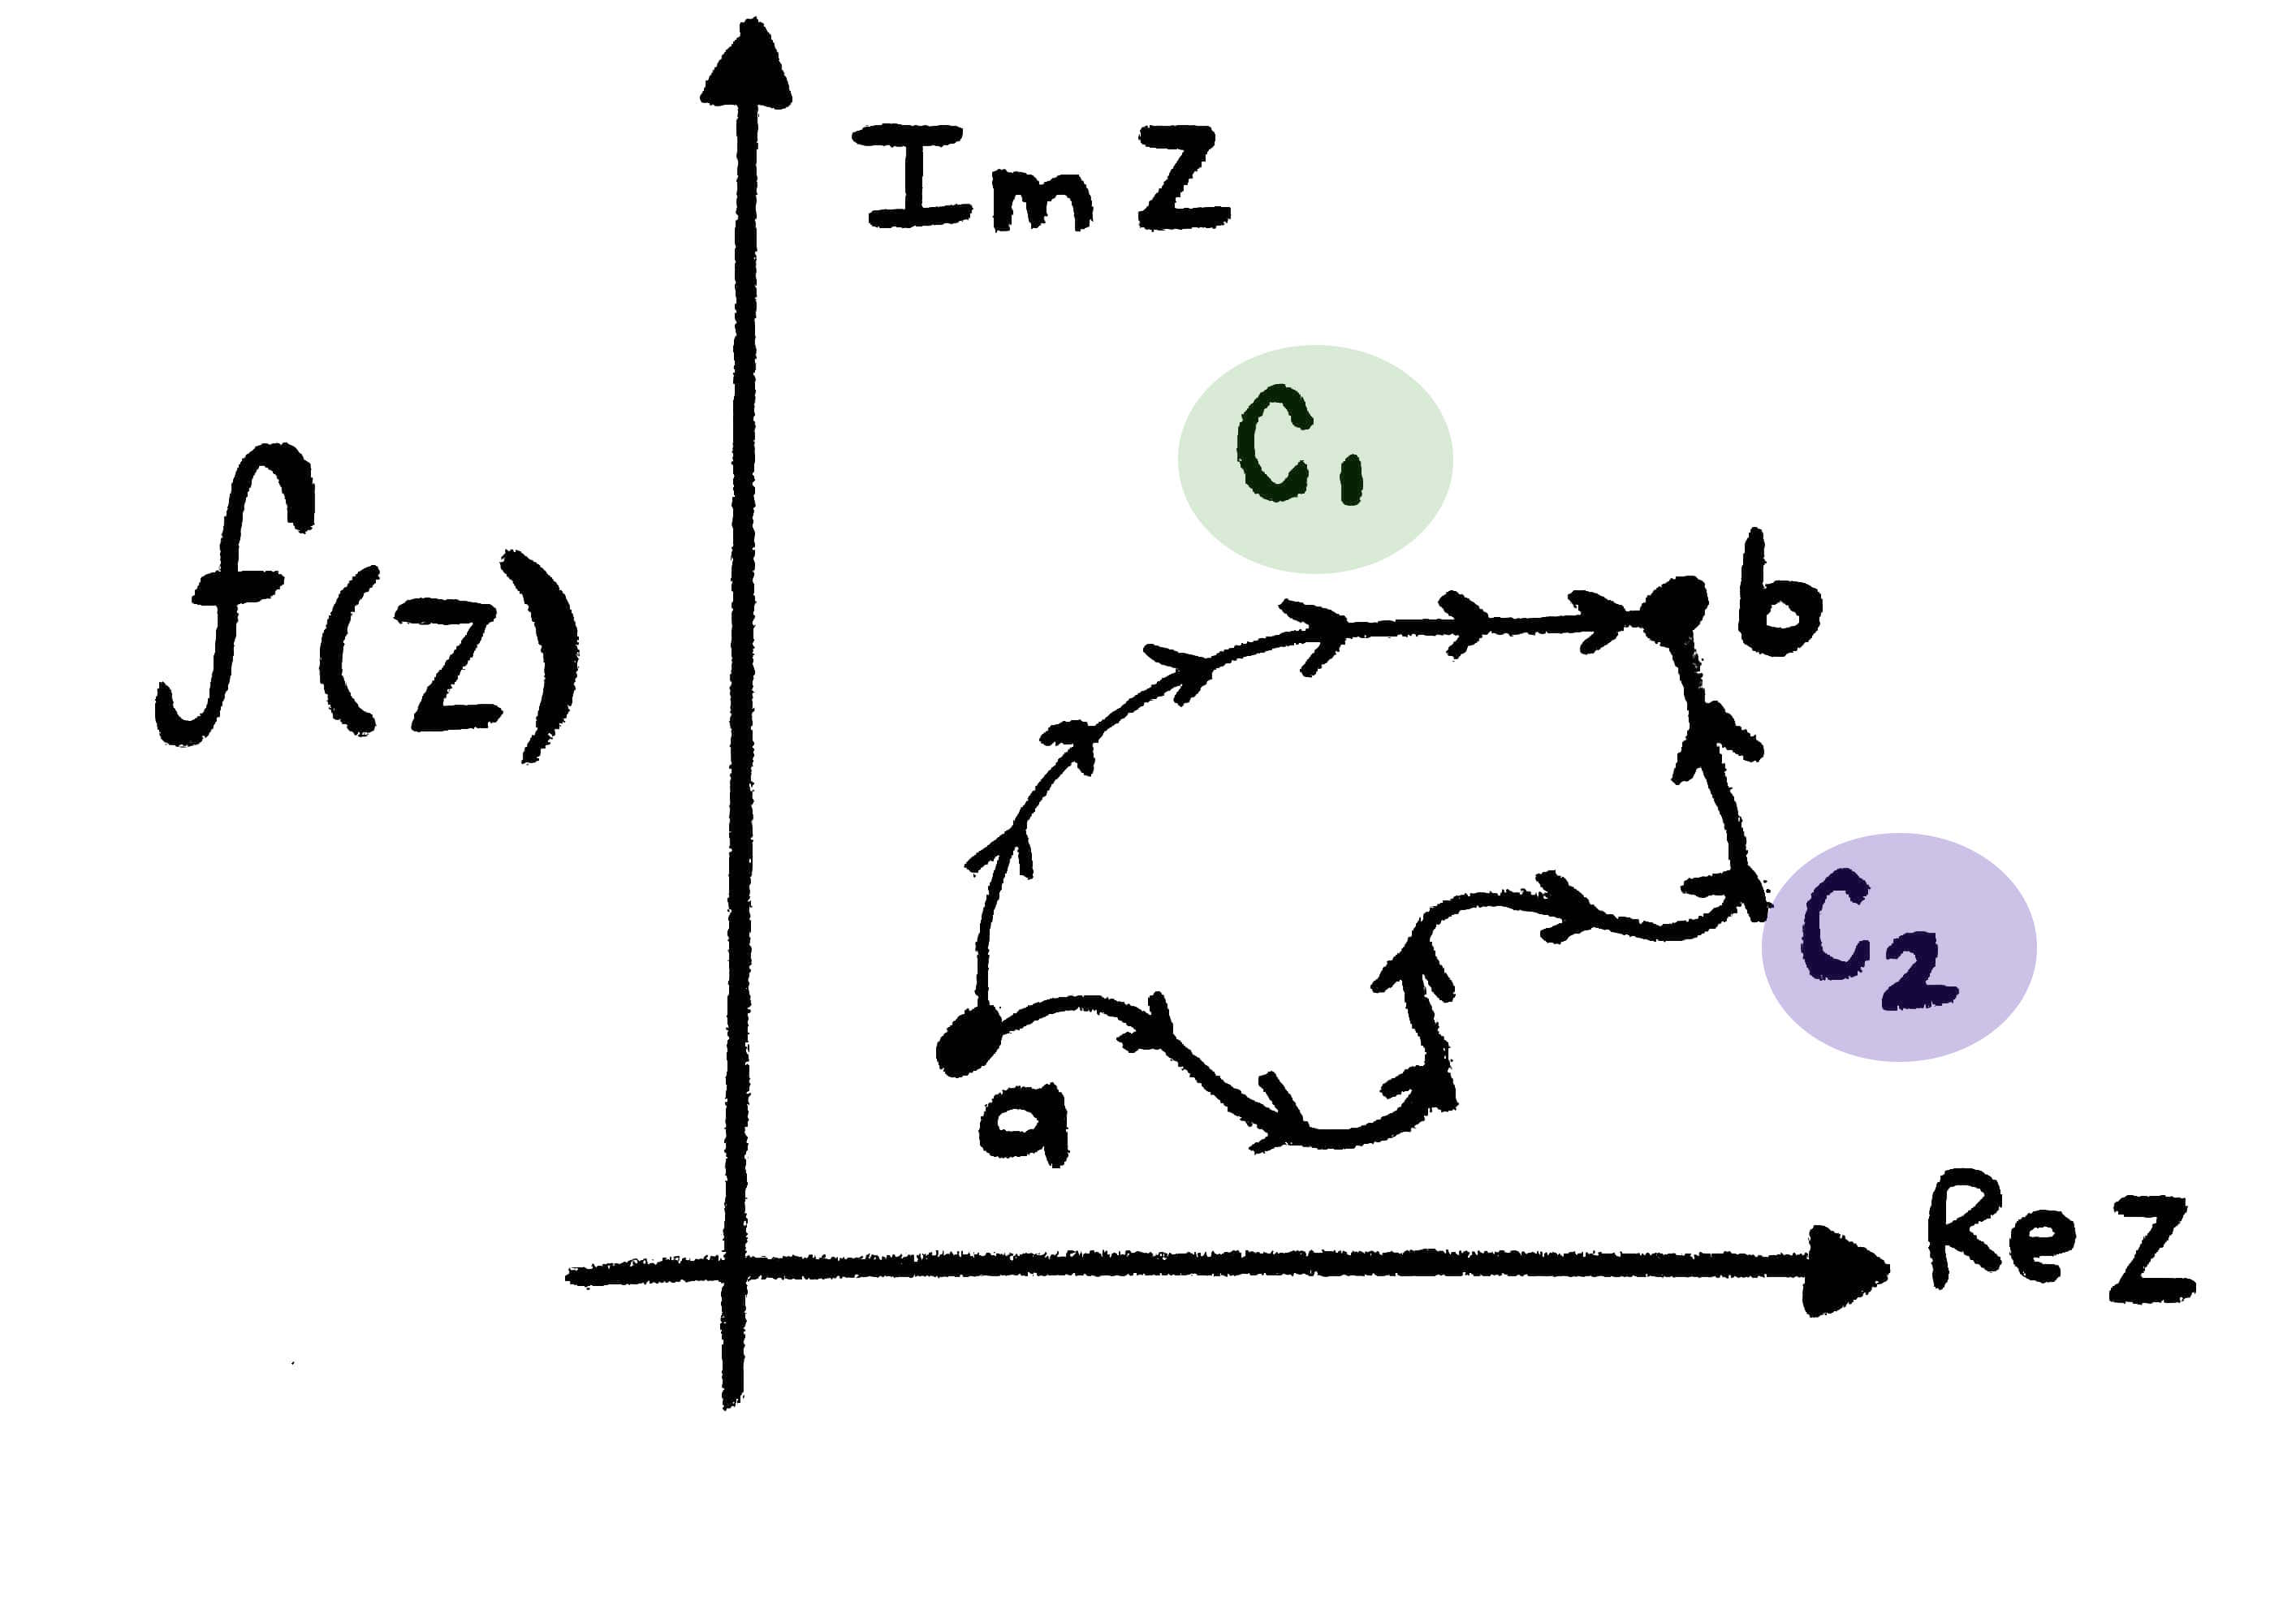
\includegraphics[width=0.43\textwidth]{CaminosDeIntegralCompleja.jpg}
                \caption{\scriptsize{¿Qué camino sigo? $C_1$ ó $C_2$}}
            \end{wrapfigure}

            Y el gran problema es que cada camino podría darte un valor diferente
            al momento de calcular la integral.

            Así que para integrar una función compleja es necesario que me digas
            cual será la curva por la cual integraremos dicha función, debido a esto
            hay grandes relaciones sobre como funciona una integral compleja y una 
            integral de línea.

            Esto se debe basicamente a que los números complejos no viven en una línea, 
            una recta númerica, sino en todo un plano complejo.


            % ==============================================
            % ========          INTEGRALES         =========
            % ==============================================
            \clearpage
            \subsection{Calcular un Integral Compleja sobre $C$}


                Supongamos que tenemos una función $f(z) = u_{(x,y)} + iv_{(x,y)}$
                sobre una curva arbitraria $\mathcal{C}$ desde el punto $a$ hasta $b$

                Supongamos que dicha curva se puede expresar usando ecuaciones parametricas
                de tal manera que $x,y$ son funciones de un párametro $t$ tal que
                así: $x(t)$ y $y(t)$.

                Entonces tenemos que podemos expresar a $a$ y a $b$ como:
                \begin{itemize}
                    \item $a = x(\alpha) + iy(\alpha)$
                    \item $b = x(\beta) + iy(\beta)$
                \end{itemize}

                Entonces ya podemos definir lo que significa una integral compleja:

                \begin{MultiLineEquation*}{3}
                    \int_C f(z) dz
                    &   = \int_C f(x+iy) (dx+idy)
                    \\& = \int_C (u +iv) (dx+idy)
                    \\& = \int_C udx - vdy + i\int_c vdx + udy 
                \end{MultiLineEquation*}

                Apliquemos un cambio de variable: 
                $dx = \frac{dx}{dt} dt$ y $dy = \frac{dy}{dt} dt$

                Por lo tanto finalmento podemos decir que:
                \begin{MultiLineEquation*}{3}
                    \int_c f(z) dz 
                        &=
                        \int_\alpha^\beta u\frac{dx}{dt} dt - v\frac{dy}{dt} dt
                        + 
                        i\int_\alpha^\beta v\frac{dx}{dt} dt + u\frac{dy}{dt} dt
                    \\  &=
                        \int_\alpha^\beta u_{(x,y)} x'(t) dt - v_{(x,y)} y'(t) dt
                        + 
                        i\int_\alpha^\beta v_{(x,y)} x'(t) dt + u_{(x,y)} y'(t) dt
                \end{MultiLineEquation*}
                


            % ==============================================
            % ========     PARAMETRIZACION         =========
            % ==============================================
            \clearpage
            \subsection{Parametrización}

                Otra forma complemente igual de valida es no parametrizar las funciones
                en parte real e imaginaria.

                Entonces podemos defininir $\int_c f(z)dz$ para cualquier curva
                cerrada. Si $C$ esta parametrizada por $r(t), \; a \leq t \leq b$
                tenemos que podemos ver a $r'(t)$ como una curva compleja y:
                \begin{equation*}
                    \int_C f(z) dz = \int_a^b f(r(t)) \; r'(t) \; dt
                \end{equation*}

                O también es común ponerlo como:
                \begin{equation*}
                    \int_C f(z) dz = \int_a^b f(z(t)) \; z'(t) \; dt
                \end{equation*}


        % ==============================================
        % ==  TEOREMA DE CAUCHY DE LAS INTEGRALES   ====
        % ==============================================
        \section{Integrales Bonitas: Antiderivadas}

            Ya que hemos aprendido todo esto sobre las integrales podemos ver que el hecho
            de parametrizar simplifica enormemente todo el trabajo que tenemos que hacer sobre
            las mismas, llegando a esto tan bonito:

            Sea $z(t) = x(t) + iy(t)$ entonces suponiendo que sean continuas en $[a,b]$
            tenemos que:
            \begin{equation*}
                \int_a^b z(t) dt 
                    = \int_a^b (x(t) + iy(t))dt
                    = \int_a^b x(t)dt + i\int_a^b y(t)dt
            \end{equation*}



        % ==============================================
        % =====  TEOREMA DE LA DEFORMACION     =========
        % ==============================================
        \section{Teorema de la Deformación}

            Sea $\Gamma$ y $\gamma$ dos trayectorias cerradas en una región del plano $R$
            con $\gamma$ en el interior de $\Gamma$.

            Sea $f(z)$ una función diferenciable en un conjunto abierta que contiene ambas
            trayectorias y todos los puntos entre ellas, entonces:
            \begin{equation*}
                \oint_\Gamma f(z) dz = \oint_\gamma f(z) dz
            \end{equation*}




        % ==============================================
        % ==  TEOREMA DE CAUCHY DE LAS INTEGRALES   ====
        % ==============================================
        \clearpage
        \section{Teorema de Cauchy-Goursat}

            Si $f(z)$ es analítica y estamos hablando de una curva simple, es decir
            en la que no se cruza consigo mismo, entonces tenemos que:
            \begin{equation*}
                \oint_C f(z) dz = 0
            \end{equation*}

            % ======== DEMOSTRACION ========
            \begin{SmallIndentation}[1em]
                \textbf{Ideas}:
                
                Antes que hablar de la demostración del Teorema tenemos que recordar lo que 
                significa que una Región $R$ sea simplemente conexa.

                \Quote{Un Región $R$ es simplemente conexa si cada curva simple en $R$ es la
                frontera de una región contenida en $R$}

                De esto podemos ver que por ejemplo el disco $\Set{z \in \Complexs, \Such |z| < 1}$
                es simplemente conexo, pero el anillo $\Set{z \in \Complexs, \Such 1 < |z| < 1}$
                no lo es.


                \textbf{\\Usando el Teorema de Green}:

                Supongamos que $C$ es un curva simple cerrada que esta limitada por D
                entonces si queremos aplicar el Teorema de Green a la integral:
                $\int_C f(z) dz$ ya que tenemos que:
                \begin{MultiLineEquation*}{3}
                    f(z) dz 
                        &= (u+iv)(dx+idy)
                        &= (udx - vdy) + i (vdx + udy) 
                \end{MultiLineEquation*}
                
                Entonces podemos ver que:
                \begin{MultiLineEquation*}{3}
                    \int_C f(z) dz 
                        &=    \iint_D \Wrap{ - \Partial{v}{x} - \Partial{u}{y}} dA
                            +i\iint_D \Wrap{\Partial{u}{x} - \Partial{v}{y}} dA
                \end{MultiLineEquation*}

                Entonces el integrando será siempre cero si y solo si las ecuaciones
                de Cauchy Riemann se mantienen.
                    
            \end{SmallIndentation}
                





        % ==============================================
        % ==  TEOREMA DE LA INTEGRAL DE CAUCHY      ====
        % ==============================================
        \clearpage
        \section{Teorema de la Integral de Cauchy}

            Sea $f(z)$ analítica en el interior y sobre la frontera de $\mathcal{C}$, donde
            $\mathcal{C}$ es cerrada y simplemente conexa en una región $R$, entonces
            tenemos si $a$ pertenece a la región $R$ se cumple que:
            \begin{equation*}
                f(a) = \dfrac{1}{2 \pi i} \oint_C \dfrac{f(z)}{z-a} dz
            \end{equation*}

            Pero esta no es la forma en la que comunmente la usamos, sino que la usamos
            como un pequeño truco para poder calcular algunas integrales,
            esto lo escribimos entonces así:
            \begin{equation*}
                2 \pi i \; f(a) = \oint_C \dfrac{f(z) dz}{z-a}
            \end{equation*}






            % ==============================
            % ===   TEOREMA DE LA INTEGRAL = 
            % === VS FORMULA DE LA INTEGRAL=
            % ==============================
            \subsection{Teorema de Integral vs Formula de la Integral}
            \begin{SmallIndentation}[1em]

                Consideremos un ejemplo que creo que pone todo mas claro, 
                supon la función $f(z) = z^2 + z + 1$ a lo largo de 
                el circulo unitario.

                Por lo tanto tenemos que:
                \begin{MultiLineEquation*}{3}
                    \int_C f(z) dz 
                        &= \int_0^{2\pi} (e^{2it} + e^{it} + 1) ie^{it} dt
                        &= i \int_0^{2\pi} (e^{3it} + e^{2it} + e^{it}) dt
                \end{MultiLineEquation*}

                Creo que es muy sencillo ver que esta integral será cero, porque
                el periodo de el seno y coseno es $2\pi$, por lo tanto
                al momento de evaluar todo se cancela.

                Pero por otro lado imagina:
                \begin{MultiLineEquation*}{3}
                    \int_C \dfrac{1}{z} dz 
                        &= \int_0^{2\pi} (e^{-it}) ie^{it} dt           
                        &= i \int_0^{2\pi} dt
                        &= 2 \pi i
                \end{MultiLineEquation*}

                ¿Pero porque no dio cero?

                Porque $\dfrac{1}{z}$ es analítica en la región $\Complexs - \Set{0}$
                pero vimos que esta región no es simplemente conexa, por lo tanto no
                podemos aplicar el Teorema de Cauchy.

            \end{SmallIndentation}

                
            % ==============================
            % ========  EJEMPLO   ==========
            % ==============================
            \clearpage
            \subsection{Ejemplos}

                \begin{SmallIndentation}[1em]

                    Sea la curva aquella descrita por el circulo $|z+1|=\frac{1}{2}$
                    calcule:
                    \begin{equation*}
                        \oint_C \dfrac{dz}{z^2(z+1)}
                    \end{equation*}

                    \textbf{Solución}:

                    Simplemente tenemos que darnos cuenta que el punto de indeterminación de
                    nuestra integral es $z=0$ y $z=-1$, ahora, si te das cuenta podemos poner
                    nuestra integral como:
                    \begin{equation*}
                        \oint_C \dfrac{dz}{z^2(z- (-1))}
                    \end{equation*}

                    Entonces podemos separarlo como:
                    \begin{itemize}
                        \item $f(z) = \dfrac{1}{z^2}$
                        \item $a = -1$
                        \item $f(a) = \dfrac{1}{(-1)^2} = \dfrac{1}{1} = 1$
                    \end{itemize}

                    Por lo tanto:
                    \begin{equation*}
                        \oint_C \dfrac{dz}{z^2(z+1)} = 2 \pi i \; f(a) = 2 \pi i
                    \end{equation*}

                \end{SmallIndentation}





        % ==============================================
        % ==  TEOREMA DE DERIVACION DE ORDEN SUPERIOR ==
        % ==============================================
        \clearpage
        \section{Teorema de Cauchy de Derivación de Orden Superior}

            Sea $f(z)$ diferenciable en un conjunto $G$ entonces $f(z)$ tiene derivadas de todos
            los ordenes en cada punto de $G$, más aún si $C$ es una trayectoria cerrada en $G$
            que encierra unicamente puntos de $G$, en particular a $z_0$ tenemos que:
            \begin{equation*}
                f^{(n)}(z_0) = \dfrac{n!}{2 \pi i} \oint_C \dfrac{f(z) dz}{(z-z_0)^{n+1}}
            \end{equation*}

            Pero esta no es la forma en la que comunmente la usamos, sino que la usamos
            como un pequeño truco para poder calcular algunas integrales,
            esto lo escribimos entonces así:
            \begin{equation*}
                \dfrac{2 \pi i}{n!}f^{(n)}(z_0) = \oint_C \dfrac{f(z) dz}{(z-z_0)^{n+1}}
            \end{equation*}
                
            % ==============================
            % ========  EJEMPLO   ==========
            % ==============================
            \subsection{Ejemplos}

                \subsection*{Ejemplo 1}
                \begin{SmallIndentation}[1em]


                    Sea la curva aquella descrita por el circulo $|z|=\frac{1}{2}$
                    calcule:
                    \begin{equation*}
                        \oint_C \dfrac{dz}{z^2(z+1)}
                    \end{equation*}

                    \textbf{Solución}:

                    Simplemente tenemos que darnos cuenta que el punto de indeterminación de
                    nuestra integral es $z=0$ y $z=-1$, ahora, si te das cuenta podemos poner
                    nuestra integral como:
                    \begin{equation*}
                        \oint_C \dfrac{dz}{z^2(z+1)}
                    \end{equation*}

                    Entonces podemos separarlo como:
                    \begin{itemize}
                        \item $n=1$
                        \item $f(z) = \dfrac{1}{z+1}$
                        \item $f'(z) = -\dfrac{1}{(z+1)^2}$
                        \item $z_0 = 0$
                        \item $f'(z_0) = -\dfrac{1}{1^2} = -1$
                    \end{itemize}

                    Por lo tanto:
                    \begin{equation*}
                        \oint_C \dfrac{dz}{z^2(z+1)} 
                            = \dfrac{2 \pi i}{n!}f^{(n)}(z_0)
                            = (2 \pi i) -1
                            = -2 \pi i
                    \end{equation*}

                \end{SmallIndentation}

                \clearpage


                \subsection*{Ejemplo 2}
                \begin{SmallIndentation}[1em]

                    Sea la curva aquella descrita por el circulo $|z|=3$
                    calcule:
                    \begin{equation*}
                        \oint_C \dfrac{dz}{z^2(z+1)}
                    \end{equation*}

                    \textbf{Solución}:

                    Ya que nuestra curva encierra a ambos puntos de indeterminación tenemos que 
                    separarla:
                    \begin{MultiLineEquation*}{3}
                        \dfrac{dz}{z^2(z+1)} &= \dfrac{Az + B}{z^2} + \dfrac{C}{z+1}     \\
                        1 &= (Az + B)(z+1) + z^2(C)                                      \\
                        1 &= Az^2 + Bz + Az + B + Cz^2
                    \end{MultiLineEquation*}

                    Por lo tanto:
                    \begin{MultiLineEquation*}{3}
                        A + C = 0
                        \Space
                        \Space
                        A + B = 0
                        \Space
                        \Space
                        B = 1
                    \end{MultiLineEquation*}

                    Es decir:
                    \begin{MultiLineEquation*}{3}
                        A = -1
                        \Space
                        \Space
                        B = 1
                        \Space
                        \Space
                        C = 1
                    \end{MultiLineEquation*}

                    Entonces podemos separarlo como:
                    \begin{MultiLineEquation*}{3}
                        \oint_C \dfrac{dz}{z^2(z+1)}
                            &= \oint_C \dfrac{Az + B}{z^2} dz + \oint_C \dfrac{C}{z+1} dz                    
                        \\  &= \oint_C \dfrac{-(z)dz}{z^2} + \oint_C \dfrac{dz}{z^2} + \oint_C \dfrac{dz}{z+1}
                        \\  &= \oint_C \dfrac{-dz}{z} + \oint_C \dfrac{dz}{z^2} + \oint_C \dfrac{dz}{z+1}
                    \end{MultiLineEquation*}
                    \clearpage

                    Ahora vamos a ir resolviendo una por una:
                    \begin{itemize}
                        \item
                            La primera se puede resolver con la Teorema de la Integral de Cauchy
                            pues tenemos que:
                            \begin{itemize}
                                \item $f(z) = -1$
                                \item $f(0) = -1$
                            \end{itemize}

                            Por lo tanto:
                            \begin{MultiLineEquation*}{3}
                                \oint_C \dfrac{-dz}{z} = 2 \pi i f(0) = -2 \pi i
                            \end{MultiLineEquation*}


                        \item
                            La segunda se puede resolver con la Teorema de Derivación Superior
                            pues tenemos que:
                            \begin{itemize}
                                \item $f(z) = 1$
                                \item $f'(z) = 0$
                            \end{itemize}

                            Por lo tanto:
                            \begin{MultiLineEquation*}{3}
                                \oint_C \dfrac{dz}{z^2} = \dfrac{2 \pi i}{n!} 0 = 0 
                            \end{MultiLineEquation*}


                        \item
                            La tercera se puede resolver con la Teorema de la Integral de Cauchy
                            pues tenemos que:
                            \begin{itemize}
                                \item $f(z) = 1$
                                \item $f(-1) = 1$
                            \end{itemize}

                            Por lo tanto:
                            \begin{MultiLineEquation*}{3}
                                \oint_C \dfrac{dz}{z+1} = 2 \pi i f(-1) = 2 \pi i
                            \end{MultiLineEquation*}
                            
                    \end{itemize}

                    Finalmente tenemos entonces que:
                    \begin{MultiLineEquation*}{5}
                        \oint_C \dfrac{dz}{z^2(z+1)}
                            &= \oint_C \dfrac{-dz}{z} &&+ \oint_C \dfrac{dz}{z^2} &&+ \oint_C \dfrac{dz}{z+1}
                        \\  &= -2 \pi i &&+ 0 &&+ 2 \pi i
                        \\  &= 0
                    \end{MultiLineEquation*}  
                \end{SmallIndentation}




% //////////////////////////////////////////////////////////////////////////////////////////////////////////
% ///////////////////////////////////        SERIES COMPLEJAS       ////////////////////////////////////////
% //////////////////////////////////////////////////////////////////////////////////////////////////////////
\part{Series Complejas y Residuos}
\clearpage

    % ===============================================================================
    % ========================           SERIES          ============================
    % ===============================================================================
    \chapter{Series Complejas}
        \clearpage


        % ==============================================
        % ===========    SERIES GEOMETRICAS    =========
        % ==============================================
        \clearpage
        \section{Serie Geométrica}

            Si $|z| < 1$ entonces la Serie:
            \begin{MultiLineEquation*}{3}
                \sum_{n=1}^\infty az^{k-1} = \sum_{n=0}^\infty az^k
                    &= a + az + az^2 + az^3 + \dots
            \end{MultiLineEquation*}

            Converge a $\dfrac{a}{1 - z}$

            % ======== DEMOSTRACION ========
            \begin{SmallIndentation}[1em]
                \textbf{Demostración}:

                Ahora podemos encontrar una expresión para la suma parcial $S_n$ como:\\
                $S_n = a + az + az^2 + az^3 + \dots + az^{n-1}$.

                Ahora el gran truco para poder evaluar más sencillo $S_n$ lo que podemos hacer
                es:
                \begin{MultiLineEquation*}{3}
                    S_n         &= a  + az   + az^2 + az^3 + \dots + az^{n-1}       \\
                    zS_n        &= az + az^2 + az^3 + az^4 + \dots + az^n           \\
                    S_n - zS_n  &= (a  + az   + az^2 + az^3 + \dots + az^{n-1})     
                                    -
                                   (az + az^2 + az^3 + az^4 + \dots + az^n)         \\
                    S_n - zS_n  &= a - az^n                                         \\
                    S_n(1 - z)  &= a - az^n                                         \\
                    S_n         &= \dfrac{a(1 - z^n)}{1 - z}                      
                \end{MultiLineEquation*}

                Ahora $\lim_{n \to \infty} z^n = 0$ siempre que $|z| < 1$, entonces:
                \begin{MultiLineEquation*}{3}
                    \lim_{n \to \infty} \dfrac{a(1 - z^n)}{1 - z} 
                        &= \dfrac{a(1 - 0)}{1 - z}                                  \\
                        &= \dfrac{a}{1 - z}
                \end{MultiLineEquation*}
            
            \end{SmallIndentation}
                


        % ==============================================
        % ===========    SERIES DE POTENCIAS   =========
        % ==============================================
        \clearpage
        \section{Series de Potencias}

            Una serie de Potencias es una serie de la forma:
            \begin{MultiLineEquation*}{3}
                \sum_{n=0}^\infty a_k (z - z_0)^k
                    &= a_0 + a_1(z-z_0) + a_2(z-z_0)^2 + a_3(z-z_0)^3 + \dots 
            \end{MultiLineEquation*}

            Ahora, hay muchas cosas que debes saber, muchos nombres y designaciones que hacemos a 
            las series de potencias:

            \begin{itemize}

                \item Se dice que la Serie centrada en $z_0$

                \item Hablamos de un radio de convergencia de dicha serie, el radio puede ser:
                    \begin{itemize}
                        \item El radio es 0, entonces decimos que solo converge en $z=z_0$
                        \item El radio es finito, entonces la serie converge siempre que $z$
                            este dentro del radio
                        \item El radio es infinito, en ese cado siempre converge
                     \end{itemize}

                \item Es conveniente decir que $(z-z_0)^0 = 1$ incluso cuando $z = z_0$

                \item La corresponcia entre un número complejo $z$ que se encuentre dentro
                    del círculo de convergencia y en número $w$ al cual converge la serie
                    $\sum_{n=0}^\infty a_k (z - z_0)^k$ es de uno a uno.

                    Por lo tanto podemos ver a una serie de convergencia como una función $f(z) = w$
            \end{itemize}




            
                
                

        % ==============================================
        % ===========    TEOREMA DE TAYLOR     =========
        % ==============================================
        \clearpage
        \section{Series de Taylor}

            Sea $f(z)$ análitica en el interior de un círculo $C_0$ con centro en $z_0$
            y radio $r_0$. Entonces para cada punto $z$ en el interior de $C_0$ se tiene
            que $f(z)$ se puede escribir como:
            \begin{equation*}
                f(z)    
                    = \sum_{n=0}^\infty a_n (z-z_0)^n
                    = \sum_{n=0}^\infty \dfrac{f^{(n)}(z_0)}{n!} (z-z_0)^n
            \end{equation*}

            Además para cualquier círculo en el interior de $C_0$ la serie converge
            uniformemente.

            % ======== DEMOSTRACION ========
            \begin{SmallIndentation}[1em]
                \textbf{Ideas}:

                    Podemos diferenciar a una serie de potencias simplemente diferenciando término por término,
                    y como creo que es más que obvio, el diferenciar una serie de potencias no hace que cambie 
                    su radio de convergencia.

                    Es decir, una serie de pontencia define a una función infinitamente derivable que tendrá
                    el mismo radio de convergencia. 


                    Ahora, veamos que pasa el derivar una serie de potencia:\\
                    $f(z) = \sum_{n=0}^\infty a_k (z - z_0)^k = a_0 + a_1(z-z_0) + a_2(z-z_0)^2 + \dots$


                    \begin{MultiLineEquation*}{3}
                        f'(z) 
                                &= \sum_{n=0}^\infty a_k \; k(z - z_0)^{k-1}            
                                &&= a_1 + 2a_2(z-z_0) + 3a_3(z-z_0)^2 + \dots           \\
                        f''(z) 
                                &= \sum_{n=0}^\infty a_k \; (k)(k-1)(z - z_0)^{k-2}     
                                &&= (2)(1)a_2 + (3)(2)a_3(z-z_0) + \dots                \\
                        f'''(z)                                                         
                                &= \sum_{n=0}^\infty a_k \; (k)(k-1)(k-2)(z - z_0)^{k-3} 
                                &&= (3)(2)a_3 + \dots                                
                    \end{MultiLineEquation*}

                    Hay una relación entre los coeficientes de $a_k$ y la derivadas de $f(z)$, entonces
                    tenemos que $f(z_0) = a_0$, $f'(z_0) = 1!(a_1)$, $f''(z_0) = 2!(a_2)$, $f'''(z_0) = 3!(a_3)$.

                    Entonces en general tenemos que $\UpperDerivate{f(z)}{z}{n} = (n!) a_n$

                    Con lo que con un simple despeje tenemos que $a_n = \dfrac{f^{(n)} (z_0)}{n!}$

                    Por lo tanto tenemos que:
                    \begin{equation*}
                        f(z) = \sum_{n=0}^\infty \dfrac{f^{(n)}(z_0)}{n!} (z-z_0)^n
                    \end{equation*}
            
            \end{SmallIndentation}



            % =========================================
            % =========    SERIES FAMOSAS     =========
            % =========================================
            \clearpage
            \subsection{Series de Taylor Famosas}

                \begin{MultiLineEquation*}{3}
                    e^z = \sum_{n=0}^\infty \dfrac{z^n}{n!}
                \end{MultiLineEquation*}

                \begin{MultiLineEquation*}{3}
                    sen(z) = \sum_{n=0}^\infty \dfrac{z^{2n+1}}{(2n+1)!} (-1)^n
                \end{MultiLineEquation*}

                \begin{MultiLineEquation*}{3}
                    cos(z) = \sum_{n=0}^\infty \dfrac{z^{2n}}{(2n)!} (-1)^n
                \end{MultiLineEquation*}

                \begin{MultiLineEquation*}{3}
                    a\pfrac{1}{1-z} = \sum_{n=0}^\infty a (z^n) \Space \text{si } |z| < 1 
                \end{MultiLineEquation*}

                \begin{MultiLineEquation*}{3}
                    a\pfrac{1}{1+z} = \sum_{n=0}^\infty a (z^n)(-1)^{n-1} \Space 
                    \text{si } |z| < 1 
                \end{MultiLineEquation*}

                \begin{MultiLineEquation*}{3}
                    (1-z)^n = \sum_{n=0}^\infty \binom{n}{r} z^{n-r}
                \end{MultiLineEquation*}
                    


        % ==============================================
        % ===========    SERIES DE MACLAURIN    ========
        % ==============================================
        \section{Series de Maclaurin}

            Si $z_0 = 0$ entonces la Serie de Taylor recibe un nombre especial
            \begin{equation*}
                f(z) = \sum_{n=0}^\infty \dfrac{f^{(n)}(0)}{n!} z^n
            \end{equation*}

            Y si, eso es todo, una Serie de Taylor con $z_0 = 0$. 






        % ==============================================
        % ===========    SERIES DE LAURENT      ========
        % ==============================================
        \clearpage
        \section{Series de Laurent}

            Si $z = z_0$ es una singularidad aislada de una función $f(z)$ entonces tenemos
            que podemos escribir a la función como:
            \begin{equation*}
                \sum_{-\infty}^\infty a_{n}(z - z_0)^n
            \end{equation*}

            % ======== DEMOSTRACION ========
            \begin{SmallIndentation}[1em]
                \textbf{Ideas}:
                
                Si una función no es analítica en el punto $z = z_0$, entonces
                en este punto decimos que tenemos una singularidad o un punto singular de la
                función.

                Ahora vamos a ver un nuevo tipo de las Series de Potencias de $f(z)$ sobre
                una singularidad aislada sobre $z_0$.
                Esta nueva serie involucrará a potencias positivas como no negativas de $(z - z_0)$.

                Si $z = z_0$ es una singularidad de una función $f(z)$ entonces es muy obvio que
                no podemos expandirla como una Serie de Potencias común con $z_0$ en su centro.

                Pero si $z = z_0$ es una singularidad aislada entonces podemos representarla como
                una Serie Potencias que involucra potencias negativas y positivas.

                \begin{MultiLineEquation*}{3}
                    f(z) 
                        &= \cdots + \dfrac{a_{-2}}{(z - z_0)^2} + \dfrac{a_{-1}}{(z - z_0)^1}
                            &&+ a_0 + a_1(z - z_0)^1 + + a_2(z - z_0)^2 + \cdots            \\
                        &= \sum_{n=1}^\infty a_{-n}(z - z_0)^{-n} 
                            &&+
                           \sum_{n=0}^\infty a_{n}(z - z_0)^n                               \\
                        &= \sum_{-\infty}^\infty a_{n}(z - z_0)^n
                \end{MultiLineEquation*}

                Llamamos a la parte $\sum_{n=0}^\infty a_{n}(z - z_0)^n$ como la parte principal,
                y decimos que esta suma converge si $|z - z_0| > r$

                La parte $\sum_{n=1}^\infty a_{-n}(z - z_0)^{-n}$como la parte análitica
                y decimos que esta suma converge si $|z - z_0| < R$
            
            \end{SmallIndentation}


            % =====================================
            % ====   COEFICIENTES DE LAURENT   ====
            % =====================================
            \clearpage
            \subsection{Coeficientes de la Serie de Laurent}

                Podemos encontrar facilmente los coeficientes de una Serie de Taylor como:\\
                $a_n = \frac{f^{(n)}(z_0)}{n!}$

                Podemos hacer algo parecido con las Series de Laurent y decir que:

                Para la Parte Análitica tenemos que:
                \begin{equation*}
                    a_n = \dfrac{1}{2 \pi i} \oint_C \dfrac{f(z)}{(z - z_0)^{n+1}} dz
                \end{equation*}

                Para la Parte Principal tenemos que:
                \begin{equation*}
                    a_n = \dfrac{1}{2 \pi i} \oint_C \dfrac{f(z)}{(z - z_0)^{-n+1}} dz
                \end{equation*}


                Donde $C$ es cualquier curva cerrrada que rodea a $z_0$.





            % =====================================
            % ===========    EJEMPLOS      ========
            % =====================================
            \clearpage
            \subsection{Ejemplos}


                % =====================================
                % ===========    EJEMPLO 1     ========
                % =====================================
                \subsubsection{Ejemplo 1}

                    Encuentra la expansión de $f(z) = \dfrac{\Sin{z}}{z^4}$ alrededor
                    de $z = 0$

                    % ======== SOLUCIÓN ========
                    \begin{SmallIndentation}[1em]
                        \textbf{Solución}:
                        
                        Recuerda que $\Sin{z} = z - \dfrac{z^3}{3!} + \dfrac{z^5}{5!} - 
                        \dfrac{z^7}{7!} + \dots$

                        \begin{MultiLineEquation*}{3}
                            \dfrac{\Sin{z}}{z^4} = \dfrac{1}{z^3} - \dfrac{1}{3!z} + 
                            \dfrac{z}{5!} - \dfrac{z^3}{7!} + \dots
                        \end{MultiLineEquation*}

                        Donde tenemos que:
                        \begin{itemize}
                            \item Parte Analítica: $\dfrac{z}{5!} - \dfrac{z^3}{7!} + \dots$
                            \item Parte Principal: $\dfrac{1}{z^3} - \dfrac{1}{3!z}$
                        \end{itemize}
                            
                    \end{SmallIndentation}


                % =====================================
                % ===========    EJEMPLO 2     ========
                % =====================================
                \subsubsection{Ejemplo 2}

                    Encuentre la expansión de $f(z) = \dfrac{1}{z(z-1)}$ en:

                    \begin{itemize}
                        \item $0 < |z| < 1$

                            % ======== DEMOSTRACION ========
                            \begin{SmallIndentation}[1em]
                                \textbf{Demostración}:
                                
                                Estamos de acuerdo en que la Superficie $0 < |z| < 1$ representa 
                                el círculo unitario menos $z = 0$, por lo tanto tenemos una
                                superficie que encierra a un punto de singularidad.

                                Por lo tanto tenemos que hacer una expansión de $\dfrac{1}{z(z-1)}$
                                que involucre a $(z - 0)$.

                                Ahora tenemos que:
                                \begin{MultiLineEquation*}{3}
                                    f(z)
                                        &= \dfrac{1}{z(z-1)}                            \\
                                        &= \pfrac{-1}{z}\pfrac{1}{1-z}                  \\
                                        &= \pfrac{-1}{z}\Wrap{1+z+z^2+z^3+z^4+\dots}    \\
                                        &= -\pfrac{1}{z} -1 - z - z^2 - z^3 - \dots     \\
                                \end{MultiLineEquation*}

                                Sabemos que $\dfrac{1}{1-z} = \Wrap{1+z+z^2+z^3+z^4+\dots}$
                                si y solo si $|z|< 1$ y al multiplicarlo por $\dfrac{1}{z}$
                                entonces tenemos que la expresión general converge si y solo si
                                $0 < |z| < 1$.
                            \end{SmallIndentation}

                        \item $1 < |z|$

                            % ======== DEMOSTRACION ========
                            \begin{SmallIndentation}[1em]
                                \textbf{Demostración}:
                                
                                Estamos de acuerdo en que la Superficie $1 < |z|$ representa
                                todo el plano complejo excepto el círculo unitario, por lo tanto tenemos una superficie que encierra a un punto de singularidad.

                                Por lo tanto tenemos que hacer una expansión que involucre a 
                                $(z - 0)$.

                                Ahora tenemos que:
                                \begin{MultiLineEquation*}{3}
                                    f(z)
                                        &= \dfrac{1}{z(z-1)}                                \\
                                        &= \pfrac{1}{z^2}\pfrac{1}{1-\frac{1}{z}}           \\
                                        &= \pfrac{1}{z^2}\pfrac{1}{1+z+z^2+z^3+z^4+\dots}   \\
                                        &= \dfrac{1}{z^2} + \dfrac{1}{z^3} + \dfrac{1}{z^4}
                                            + \dfrac{1}{z^5} + \dots
                                \end{MultiLineEquation*}

                                La serie $1+z+z^2+z^3+z^4+\dots$ converge si y solo si 
                                $|\dfrac{1}{z}| < 1$ por lo tanto su inversa converge 
                                si y solo si $|z| > 1$
                            \end{SmallIndentation}

                        \item $0 < |z - 1| < 1$

                            % ======== DEMOSTRACION ========
                            \begin{SmallIndentation}[1em]
                                \textbf{Demostración}:
                                
                                Estamos de acuerdo en que la Superficie $0 < |z - 1| < 1$
                                representa el círculo unitario pero centrado en $z=1$, por lo
                                tanto tenemos una superficie que encierra a un punto de
                                singularidad.

                                Por lo tanto tenemos que hacer una expansión que involucre a 
                                $(z - 1)$.

                                Ahora tenemos que:
                                \begin{MultiLineEquation*}{3}
                                    f(z)
                                        &= \dfrac{1}{z(z-1)}                                \\
                                        &= \dfrac{1}{(z+1-1)(z-1)}                          \\
                                        &= \pfrac{1}{z-1}\pfrac{1}{ 1+ (z-1)}               \\
                                        &= \pfrac{1}{z-1}[1 - (z-1) + (z-1)^2 - 
                                                (z-1)^3 + (z-1)^4 - \dots]                  \\
                                        &= \pfrac{1}{z-1} + 1 + (z-1) + 
                                                (z-1)^3 + (z-1)^4 + \dots]                  \\
                                \end{MultiLineEquation*}

                                Ahora como $z \neq 1$ entonces $0 < |z-1|$, y gracias a la
                                serie geometrica tenemos que $|z-1|<1$, por lo tanto
                                la expresión converge si $0 < |z-1| < 1$

                            \end{SmallIndentation}
                            
                    \end{itemize}


            % =====================================
            % ====    POLOS Y SINGULARIDADES   ====
            % =====================================
            \subsection{Polos y Singularidades Aisladas}

                Supongamos que tenemos una función como:
                \begin{MultiLineEquation*}{3}
                    f(z) 
                    &= \sum_{-\infty}^\infty a_{n}(z - z_0)^n                               \\
                    &= \sum_{n=1}^\infty a_{-n}(z - z_0)^{-n} 
                        + \sum_{n=0}^\infty a_{n}(z - z_0)^n
                \end{MultiLineEquation*}

                Y que $z = z_0$ es nuestra singularidad.

                \begin{itemize}
                    \item Si la parte principal de nuestra Serie de Laurent \textbf{no tiene elementos}
                        entonces decimos que existe una \textbf{Singularidad Removible}.
                        \begin{equation*}
                            a_0 + a_1(z-z_0) + a_2(z-z_0)^2 + \cdots
                        \end{equation*}

                    \item Si la parte principal de nuestra Serie de Laurent \textbf{tiene una cantidad
                        finita de elementos} entonces decimos que tenemos un \textbf{Polo de Orden $n$}.

                        Si es que tenemos solo un elemento decimos que es un Polo Simple
                        \begin{equation*}
                            a_{-n}(z - z_0)^{-n} + \cdots + a_{-1}(z - z_0)^{-1} + 
                            a_0 + a_1(z-z_0) + a_2(z-z_0)^2 + \cdots
                        \end{equation*}

                    \item Si la parte principal de nuestra Serie de Laurent \textbf{tiene una cantidad
                        infinita de elementos} entonces decimos que tenemos una \textbf{Singularidad
                        Escencial} 
                        \begin{equation*}
                            \cdots + a_{-2}(z - z_0)^{-2} + a_{-1}(z - z_0)^{-1} +
                            a_0 + a_1(z-z_0) + a_2(z-z_0)^2 + \cdots
                        \end{equation*}
                \end{itemize}







    % ===============================================================================
    % ========================           RESIDUOS        ============================
    % ===============================================================================
    \chapter{Residuos} 
        \clearpage

            % ==============================================
            % ===========        DEFINICION        =========
            % ==============================================
            \section{Definición}

                Supongamos que tenemos una función como:
                \begin{MultiLineEquation*}{3}
                    f(z) 
                    &= \sum_{-\infty}^\infty a_{n}(z - z_0)^n                               \\
                    &= \sum_{n=1}^\infty a_{-n}(z - z_0)^{-n} 
                        + \sum_{n=0}^\infty a_{n}(z - z_0)^n
                \end{MultiLineEquation*}

                Entonces en especial el primer coeficiente ($a_{-1}$) es tan especial que recibe
                el nombre de residuo.

                Solemos denotar el Residuo de $f(z)$ sobre el punto $z = z_0$ como:
                \begin{equation*}
                    a_{-1} = Res(f(z), z_0)
                \end{equation*}


            % ==============================================
            % ======     ENCONTRAR RESIDUOS        =========
            % ==============================================
            \clearpage
            \section{Encontrar Residuos}

                \begin{itemize}

                    \item
                        La forma más trivial de encontrar nuestro residuo sobre $f(z)$
                        a lo largo de un punto $z_0$ es simplemente hayar la Serie de Laurent
                        de dicha función y tomar el coeficiente de $\dfrac{a_{-1}}{z-z_0}$.

                        No tengo que demostrar esto, despúes de todo esta es la definición


                    \item
                        Vimos que encontramos una fórmula para encontrar un coeficiente arbitario
                        dentro de la Serie de Laurent, esta fórmula funciona para encontrar a
                        los términos de la Parte Principal:
                        $a_n = \frac{1}{2 \pi i} \oint_C \frac{f(z)}{(z - z_0)^{-n+1}} dz$

                        Entonces:
                        \begin{MultiLineEquation*}{3}
                            a_{-1} = \dfrac{1}{2 \pi i} \oint f(z) dz
                        \end{MultiLineEquation*}
                            
                    
                    \item 
                        Si $f(z)$ tiene un Polo Simple en $z = z_0$, entonces
                        tenemos que:
                        \begin{equation*}
                            Res(f(z), z_0) = \lim_{z \to z_0} (z - z_0) f(z)
                        \end{equation*} 

                        % ======== DEMOSTRACION ========
                        \begin{SmallIndentation}[1em]
                            \textbf{Demostración}:
                            
                            Considera que $z_0$ es un Polo Simple, entonces la función
                            tiene esta forma:
                            $\dfrac{a_{-1}}{z-z_0} a_0 + a_1(z - z_0)^1 
                                        + a_2(z - z_0)^2 + \dots$

                            Donde $a_{-1}$ es diferente de cero. Ahora simplemente al
                            multiplicar todo por $(z-z_0)$ y más aún tomando el
                            límite tenemos que:
                            $\lim_{z \to z_0} (z - z_0) f(z)
                                    = \lim_{z \to z_0} [a_{-1} + a_0(z - z_0) 
                                        + a_1(z - z_0)^2 + \dots]           
                                    = a_1$
                                
                        \end{SmallIndentation}


                    \item 
                        Si $f(z)$ tiene un Polo de Orden $n$ en $z = z_0$, entonces
                        tenemos que:
                        \begin{equation*}
                            Res(f(z), z_0) = \pfrac{1}{(n-1)!} \;
                                \lim_{z \to z_0} \MiniUpperDerivate{z}{n-1}(z - z_0)^n f(z)
                        \end{equation*} 


                    \item 
                        Si $f(z)$ se puede escribir como $f(z) = \dfrac{g(z)}{h(z)}$
                        y $g(z_0) \neq 0$ entonces tenemos que podemos encontrar el residuo de un
                        polo simple como:
                        \begin{equation*}
                            Res(f(z), z_0) = \dfrac{g(z_0)}{h'(z_0)}
                        \end{equation*}

                            
                \end{itemize}



            % =====================================
            % ===========    EJEMPLOS      ========
            % =====================================
            \clearpage
            \section{Ejemplos sobre Encontrar Residuo}


                % =====================================
                % ===========    EJEMPLO 1     ========
                % =====================================
                \subsubsection{Ejemplo 1}

                    Encuentra los residuos de $f(z) = \dfrac{1}{(z-1)^2 (z-3)}$

                    % ======== SOLUCIÓN ========
                    \begin{SmallIndentation}[1em]
                        \textbf{Solución}:
                        
                        \begin{itemize}
                            \item
                                Para $z = 3$ vemos un Polo Simple por lo que podemos
                                decir que:
                                \begin{MultiLineEquation*}{3}
                                    Res(f(z), 3)
                                        &= \lim_{z \to 3} (z - 3) f(z)                          \\
                                        &= \lim_{z \to 3} (z - 3) \dfrac{1}{(z-1)^2 (z-3)}
                                            = \lim_{z \to 3} \dfrac{1}{(z-1)^2}                 \\
                                        &= \dfrac{1}{(3-1)^2} = \dfrac{1}{2^2} = \dfrac{1}{4}   
                                \end{MultiLineEquation*}

                            \item
                                Para $z = 1$ vemos un Polo de Orden 2 por lo que podemos
                                decir que:
                                \begin{MultiLineEquation*}{3}
                                    Res(f(z), 1)
                                        &= \lim_{z \to 1} \dfrac{1}{1!} 
                                            \MiniDerivate[z] (z - 1)^2 f(z)                     \\
                                        &= \lim_{z \to 1} 
                                            \MiniDerivate[z] (z - 1)^2 \dfrac{1}{(z-1)^2 (z-3)} \\
                                        &= \lim_{z \to 1} \MiniDerivate[z] \dfrac{1}{z-3}       \\
                                        &= \lim_{z \to 1} \dfrac{-1}{(z-3)^2}                   \\
                                        &= -\dfrac{1}{4}                   
                                \end{MultiLineEquation*}
                                
                        \end{itemize}
                            
                    \end{SmallIndentation}




            % ==============================================
            % ====   TEOREMA DE RESIDUO DE CAUCHY     ======
            % ==============================================
            \clearpage
            \section{Teorema de Residuo de Cauchy}

                Supongamos que tenemos una función que sea analítica excepto en $z_1, z_2, \dots, z_n$
                encerrados por $C$ entonces:
                \begin{MultiLineEquation*}{3}
                    \oint_C f(z) dz = 2 \pi i \sum_{i=0}^n Res(f(z), z_i)
                \end{MultiLineEquation*}




            % ========================================
            % ====   INTEGRALES TRIGONOMETRICAS   ====
            % ========================================
            \clearpage
            \section{Usar Teorema del Residuo para: $\int_0^{2\pi} F(\Cos{\theta}, \Sin{\theta}) \; d\theta$}

                La idea esta en convertir una integral de variable real en una 
                integral compleja donde nuestro recorrido será el círculo
                unitario centrado en el origen.

                El primer paso esta en parametrizar el recorrido como:
                \begin{itemize}
                    \item $z = e^{i \theta}$
                    \item $dz = ie^{i \theta} d\theta$
                    \item $d\theta  = \dfrac{dz}{ie^{i \theta}} 
                                    = \dfrac{dz}{iz}$
                    \item $\Cos{\theta} = \dfrac{e^{i \theta} + e^{-i \theta}}{2}
                                        = \dfrac{1}{2}\Wrap{z + z^{-1}}$
                    \item $\Sin{\theta} = \dfrac{e^{i \theta} + e^{-i \theta}}{2}
                                        = \dfrac{1}{2i}\Wrap{z - z^{-1}}$
                \end{itemize}

                Por lo tanto finalmente tenemos que:
                \begin{MultiLineEquation*}{3}
                    \int_0^{2\pi} F(\Cos{\theta}, \Sin{\theta}) \; d\theta
                    = \oint_C F\Wrap{
                            \dfrac{z + z^{-1}}{2}, 
                            \dfrac{z - z^{-1}}{2i} } \dfrac{dz}{iz}
                \end{MultiLineEquation*}


                % =====================================
                % ===========    EJEMPLOS      ========
                % =====================================
                \clearpage
                \subsection{Ejemplo}


                Calcule $\int_0^{2\pi} \dfrac{1}{5 + 4\Sin{\theta}} d\theta$

                % ======== DEMOSTRACION ========
                \begin{SmallIndentation}[1em]
                    \textbf{Solución}:
                    
                    \begin{MultiLineEquation*}{3}
                        \int_0^{2\pi} \dfrac{1}{5 + 4\Sin{\theta}} d\theta
                            &= \oint_C \dfrac{1}{5 + \dfrac{4}{2i}\Wrap{z - z^{-1}}} \dfrac{dz}{iz}     \\
                            &= \oint_C \dfrac{1}{2z^2 + 5iz - 2} \dfrac{dz}{iz}                         \\
                            &= \oint_C \dfrac{1}{(2z+4i)(2z+i)} \dfrac{dz}{iz}                          \\
                    \end{MultiLineEquation*}

                    Ahora usemos el Teorema de Residuo, recuerda que nuestro recorrido es alrededor del
                    círculo unitario, ve que solo uno de las raíces cae dentro del círculo unitario.
                    (z = -0.5i) pues la otra es $z = -2i$.
                    \begin{MultiLineEquation*}{3}
                        Res\Wrap{f(z), -0.5i}
                            &= \lim_{z \to -0.5i} (z+0.5i) f(z)                             \\
                            &= \lim_{z \to -0.5i} (z+0.5i)\dfrac{1}{(2z+4i)(2z+i)}          \\
                            &= \lim_{z \to -0.5i} (z+0.5i)\dfrac{1}{(2z+4i)(z+0.5i)}        \\
                            &= \lim_{z \to -0.5i} \dfrac{1}{(2z+4i)}                        \\
                            &= \lim_{z \to -0.5i} \dfrac{1}{3i}                             \\
                    \end{MultiLineEquation*}
                        
                    Ahora simplemente tenemos que:
                    \begin{MultiLineEquation*}{3}
                        \int_0^{2\pi} \dfrac{1}{5 + 4\Sin{\theta}} d\theta
                            &= \oint_C \dfrac{1}{(z+2i)(2z+1)} \dfrac{dz}{iz}               \\
                            &= 2 \pi i \Wrap{Res(f(z), -0.5i)}                              \\
                            &= 2 \pi i  \pfrac{1}{3i}                                       \\
                            &= \pfrac{2 \pi}{3} 
                    \end{MultiLineEquation*}
                        
                
                \end{SmallIndentation}
                    

            % ========================================
            % ======   VALOR PRINCIPAL DE CAUCHY   ===
            % ========================================
            \clearpage
            \section{Valor Principal de Cauchy}

                El Valor Principal de Cauchy de una intregral impropia es simplemente:
                \begin{MultiLineEquation*}{3}
                    \text{P.V }\;
                    \int_{-\infty}^\infty f(x) dx 
                        &= \lim_{R \to \infty} \int_R^R f(x) dx 
                \end{MultiLineEquation*}


                \begin{itemize}
                    \item A veces existe el Valor Principal de Cauchy cuando la integral diverge
                    
                    \item Si la integral converge entonces el Valor Principal será igual a la solución
                        de la integral original

                    \item Si $f(x)$ es una función par y el Valor Principal existe entonces
                        la integral converge
                \end{itemize}
                    

            % ========================================
            % ======   INTEGRALES INFINITAS     ======
            % ========================================
            \clearpage
            \section{Usar Teorema del Residuo para: $\int_{-\infty}^\infty f(x) dx$}

                \begin{MultiLineEquation*}{3}
                    \int_{-\infty}^\infty f(x) dx
                    &= \oint_C f(z) dz                  
                    &= \int_{-R}^R f(x) dx + \int_{C_R} f(z) dz
                    &= (2 \pi i) \sum_{i=1}^n Res(f(z), z_i)
                \end{MultiLineEquation*}

                Decimos que $C$ es un semicírculo que va desde $-R$ a $R$ sobre el plano real y el semicírculo
                complejo que encierra a todos los puntos singulares reales y a alguno del par de una singularidad
                compleja (despúes de todo recuerda que las raíces complejas vienen en pares, así que el
                semicirculo solo tomará a una).

                Despúes al momento de aplicar el siguiente teorema haremos que el semicírculo tienda
                a un semicírculo infinito centrado en el origen.

                Ahora, podemos decir que $f(z) = \frac{p(z)}{q(z)}$ donde el grado de $q(z)$ es mínimo
                dos grados mayor que el de $p(z)$, entonces tenemos que: $\int_{C_R} f(z) dz \to 0$ cuando
                $R \to \infty$.

                Si esto se cumpliera, entonces tendría que:
                \begin{MultiLineEquation*}{3}
                    \int_{-R}^R f(x) dx + \int_{C_R} f(z) dz
                    &= \int_{-R}^R f(x) dx = (2 \pi i) \sum_{i=1}^n Res(f(z), z_i)
                \end{MultiLineEquation*}

                Ve que la última línea es lo que queríamos ver
                    

                % =====================================
                % ===========    EJEMPLOS      ========
                % =====================================
                \clearpage
                \subsection{Ejemplo}

                    Calcule $\int_{-\infty}^\infty \dfrac{1}{(x^2+1)(x^2+9)} dx$

                    % ======== DEMOSTRACION ========
                    \begin{SmallIndentation}[1em]
                        \textbf{Solución}:

                        Ve que si tomemos el semicírculo igual o mayor que el que encierra a $[-3,3]$ entonces
                        encerrará a todas las raices reales y al menos a una de cada par de raíces complejas.

                        Ahora tomemos un semicirculo de $[-\infty, \infty]$

                        Y recuerda que si $f(z) = \frac{p(z)}{q(z)}$ donde el grado de $q(z)$ es mínimo
                        dos grados mayor que el de $p(z)$, entonces tenemos que: $\int_{C_R} f(z) dz \to 0$ cuando
                        $R \to \infty$. 

                        \begin{MultiLineEquation*}{3}
                            \int_{-\infty}^\infty \dfrac{1}{(x^2+1)(x^2+9)} dx
                            &= \oint_C \dfrac{1}{(x^2+1)(x^2+9)} dz                                                 \\
                            &= \int_{-R}^R \dfrac{1}{(x^2+1)(x^2+9)} dx + \int_{C_R} \dfrac{1}{(z^2+1)(z^2+9)} dz   \\
                            &= \int_{-R}^R \dfrac{1}{(x^2+1)(x^2+9)} dx                                             \\
                            &= (2 \pi i) [Res(f(z), i) + Res(f(z), 3i)]                                             \\
                            &= (2 \pi i) \Brackets{\dfrac{1}{16i} + \dfrac{-1}{48i}}                                \\
                            &= \dfrac{\pi}{12} 
                        \end{MultiLineEquation*}

                        Y más aún la función es par, por lo tanto no solo calculamos el valor principal, sino 
                        la integral completa.


                    \end{SmallIndentation}






            % ========================================
            % ======   INTEGRALES INFINITAS     ======
            % ========================================
            \clearpage
            \section{Usar Teorema del Residuo para: $\int_{-\infty}^\infty Trig(\alpha x) dx$}

                Decimos $\int_{-\infty}^\infty Trig(\alpha x)dx$ para referirnos a:
                \begin{itemize}
                    \item $\int_{-\infty}^\infty \Cos{\alpha x}dx$
                    \item $\int_{-\infty}^\infty \Sin{\alpha x}dx$
                \end{itemize}


                Estan son conocidas como Integrales de Fourier, porque las vemos de manera muy común en
                estas aplicaciones.

                Ve esto:
                \begin{MultiLineEquation*}{3}
                    \int_{-\infty}^\infty f(x) e^{i\alpha x} dx
                        &=  \int_{-\infty}^\infty f(x) \Cos{i\alpha x} dx
                            +
                            i \; \int_{-\infty}^\infty f(x) \Sin{i\alpha x} dx
                \end{MultiLineEquation*}


                % =====================================
                % ===========    EJEMPLOS      ========
                % =====================================
                \clearpage
                \subsection{Ejemplo}

                    Calcule $\int_0^\infty \dfrac{x}{x^2 + 9} \Sin{x} dx$

                    % ======== DEMOSTRACION ========
                    \begin{SmallIndentation}[1em]
                        \textbf{Solución}:

                        Lo primero que hay que ver es que como es par entonces:
                        \begin{MultiLineEquation*}{3}
                            \int_0^\infty \dfrac{x}{x^2 + 9} \Sin{x} dx 
                                &= \dfrac{1}{2} \int_{-\infty}^\infty \dfrac{x}{x^2 + 9} \Sin{x} dx 
                        \end{MultiLineEquation*}

                        Así que primero calculemos $\int_{-\infty}^\infty \dfrac{x}{x^2 + 9} \Sin{x} dx$
                        o aun más general $\int_{-\infty}^\infty \dfrac{x}{x^2 + 9} e^{iz} dx$

                        Recuerda que haremos que el semicírculo tienda a infinito :D
                            
                        \begin{MultiLineEquation*}{3}
                            \oint_C \dfrac{z}{z^2 + 9} e^{iz} dz 
                            &= \int_{-R}^R \dfrac{x}{x^2 + 9} e^{ix}dx + \int_{C_R} \dfrac{z}{z^2 + 9} e^{iz} dz   \\
                            &= \int_{-R}^R \dfrac{x}{x^2 + 9} e^{ix}dx                                             \\
                            &= (2 \pi i) [Res(f(z) e^{iz}, 3i)]                                                    \\
                            &= (2 \pi i) [\dfrac{e^{-3}}{2}]                                                       \\
                            &= \dfrac{\pi}{e^3}i 
                        \end{MultiLineEquation*}

                        Ahora:
                        \begin{MultiLineEquation*}{3}
                            \int_{-\infty}^\infty \dfrac{x}{x^2 + 9} e^{ix} dx
                                =   \int_{-\infty}^\infty \dfrac{x}{x^2 + 9} \Cos{x} dx
                                    +
                                    i \int_{-\infty}^\infty \dfrac{x}{x^2 + 9} \Sin{x} dx
                                = \dfrac{\pi}{e^3}i
                        \end{MultiLineEquation*}

                        Ahora igualemos la parte imaginaria y vemos que 
                        $\int_{-\infty}^\infty \dfrac{x}{x^2 + 9} \Sin{x} dx = \dfrac{\pi}{e^3}$


                        Ahora solo recuerda lo primero que dijimos y vemos que:
                        $\int_0^\infty \dfrac{x}{x^2 + 9} \Sin{x} dx = \dfrac{\pi}{2e^3}$

                    \end{SmallIndentation}
                    




            % ========================================
            % ======   INTEGRALES INFINITAS     ======
            % ========================================
            \clearpage
            \section{Recordatorio de las Integrales de Contorno}

                Ve que si hubiera Polos dentro del plano real ($c_1, c_2, \dots, c_n$) (cosa que no consideré)
                en las aplicaciones anteriores tenemos que tendremos que hacer una integral identada:
                \begin{MultiLineEquation*}{3}
                    \lim_{r \to 0} \int_{C_r} f(z) dz = (\pi i) \sum_{i = 1}^n Res(f(z), c_i)
                \end{MultiLineEquation*}

                Es decir, si tienes Polos en la línea real, entonces al aplicar el Teorema del 
                Residuo tendrás que:\\
                $(\pi i) \sum_{i = 1}^n Res(f(z), c_i) + (2\pi i) \sum_{i = 1}^n Res(f(z), z_i)$

                Donde $c_1, c_2, \dots, c_n$ son polos reales y $z_1, z_2, \dots, z_n$ son polos
                complejos                    





% //////////////////////////////////////////////////////////////////////////////////////////////////////////
% //////////////////////////////       SERIES Y TRANSFORMADA DE FOURIER        /////////////////////////////
% //////////////////////////////////////////////////////////////////////////////////////////////////////////
\part{Serie y Transformada de Fourier}
\clearpage

    % ===============================================================================
    % ===================        SERIES DE Fourier          ==========================
    % ===============================================================================
    \chapter{Serie de Fourier}
        \clearpage

        % ==============================================
        % =========    COSAS A RECORDAR  ===============
        % ==============================================
        \clearpage
        \section{Cosas a Recordar}


            % ==============================
            % =====   PERIODICIDAD    ======
            % ==============================
            \subsection*{Periodicidad}

                Decimos que una función $f(t)$ es periódica, con un periodo $T$ si es que para todos
                los elementos se cumple que:
                \begin{equation*}
                    f(t + T) = f(t)
                \end{equation*}
                También es importante mencionar que por obvias razones se da que para una función
                periódica que: $f(t + kT) = f(t) \Space \forall K \in \Integers$

            % ==============================
            % ====   FRECUENCIA   ==========
            % ==============================
            \subsection*{Frecuencia}

                Decimos que la frecuencia $F$ de la función periódica $f(t)$
                es simplemente $F = \dfrac{1}{T}$

            % ==============================
            % ====   FRECUENCIA   ==========
            % ==============================
            \subsection*{Frecuencia Circular $\omega$}

                Este término es muy usado en la ingeniería y esta definido como:
                \begin{MultiLineEquation*}{3}
                    \omega = 2\pi F = \dfrac{2 \pi}{T}
                \end{MultiLineEquation*}
                También es muy común usar que $T\omega = 2\pi$
                        



        % ==============================================
        % ===========   TEOREMA DE FOURIER   ===========
        % ==============================================
        \clearpage
        \section{Teorema de Fourier}

            Sea $f(t)$ una función periódica que cumple ciertas características, 
            entonces la podemos escribir como:
            \begin{MultiLineEquation*}{3}
                f(t) 
                    &= A_0 + A_1 \Sin{\omega t + \phi_1} + A_2 \Sin{\omega t + \phi_2}
                    \dots + A_n \Sin{\omega t + \phi_n}
            \end{MultiLineEquation*}
            Donde:
            \begin{itemize}
                \item $A_n$ y $\phi_n$ son constantes 
                \item $\omega = \dfrac{2\pi}{T} = 2 \pi F$
            \end{itemize}


            Y si, ya se lo que estas pensando... ¿Donde demonios estan los cosenos?

            Recuerda que:
            \begin{MultiLineEquation*}{3}
                A_n \Sin{\omega t + \phi_n}
                    &= (A_n \Cos{\phi_n})\Cos{n\omega t} &&+ (A_n \Cos{\phi_n})\Sin{n\omega t}  \\
                    &= (a_n)\Cos{n\omega t} &&+ (b_n)\Sin{n\omega t}                            \\
            \end{MultiLineEquation*}

            y con esto podemos escribirla como creo que la conoces:
            \begin{MultiLineEquation*}{3}
                f(t) 
                    &= \dfrac{1}{2}a_0
                        + \sum_{n=1}^\infty a_n \Cos{n \omega t}
                        + \sum_{n=1}^\infty a_n \Sin{n \omega t}
            \end{MultiLineEquation*}

            Recuerda:
            \begin{itemize}

                \item
                    Decidimos poner que $a_0 = \frac{1}{2}A_0$ por algo que verás a continuación
                    y que entonces hará que todo tenga sentido.

                \item
                    Esta forma de expandir a $f(t)$ es conocida como la expansión de Fourier

                \item
                    $a_n$ y $b_n$ son conocidos como los coeficientes de Fourier.

                \item
                    Es común también ver que 
                    $e^{in \omega t} = \Cos{n \omega t} +i \Sin{n \omega t}$

            \end{itemize}
                



        % ==============================================
        % =============       BASES      ===============
        % ==============================================
        \clearpage
        \section{Base de la Serie de Fourier}

            Representar una función como una serie es algo que hacemos de manera común en matemáticas.
            Probablemente la más común son usando Series de Potencias de $x$ como:
            \begin{MultiLineEquation*}{3}
                f(x) = \sum_{n=0}^\infty a_nx^n
            \end{MultiLineEquation*}

            Por ejemplo podemos ver a la función exponencial como:
            \begin{MultiLineEquation*}{3}
                e^x
                    = \sum_{n=0}^\infty \dfrac{x^n}{n!}          
                    = 1 + x + \dfrac{x^2}{2!} + \dfrac{x^3}{3!} + \dots    
                \end{MultiLineEquation*}

            Y si te das cuenta damos por sentado que estamos usando una base para dicha expansión, la
            base es en este caso las potencias de $x$: $x^0, x^1, x^2, x^3, \dots$.

            \subsubsection{Base de un Espacio Vectorial}

                Dado un espacio vectorial, decimos que $S$, un conjunto de vectores
                $S = v_1, v_2, \dots$ son base del espacio vectorial si es que podemos
                mediante combinaciones lineales de ellos alcanzar cualquier vector del
                espacio y todos son linealmente independientes entre si

            \subsubsection{Ortogonalidad}

                Un conjunto de vectores $S = v_1, v_2, \dots$ son Ortogonales 
                si y solo si $\forall i \; v_i \cdot v_j = 0$ si $i \neq j$

            \subsubsection{Ortonormal}

                Un conjunto de vectores $S = v_1, v_2, \dots$ son Ortonormales 
                si y solo si:
                \begin{itemize}
                    \item $\forall i \; v_i \cdot v_j = 0$ si $i \neq j$
                    \item $\forall i \; |v_i| = 1$
                \end{itemize}

            Podemos también usar que:
            \begin{MultiLineEquation*}{3}
                <f(x), g(x)> = \int_{-\infty}^\infty f(x)g(x) dx     
            \end{MultiLineEquation*}

            \clearpage

            Lo siguiente demuestra que $\Set{1, \Cos{\omega t}, \Cos{2 \omega t}, \dots,
            \Cos{n \omega t}, \Sin{\omega t}, \Sin{2 \omega t}, \dots, \Sin{n \omega t}}$
            Es una base ortogonal:
            \begin{itemize}
                \item
                    ${\displaystyle
                    \int_d^{d+T} \Cos{n \omega t} dt = 
                    \begin{cases}
                        0 &\Space n \neq 0  \\
                        T &\Space n = 0
                    \end{cases}
                    }$

                \item
                    ${\displaystyle
                    \int_d^{d+T} \Sin{n \omega t} dt = 0
                    }$

                \item
                    ${\displaystyle
                    \int_d^{d+T} \Sin{m \omega t} \Sin{n \omega t} \; dt =
                    \begin{cases}
                        0               &\Space m \neq n  \\
                        \dfrac{T}{2}    &\Space m = n \neq 0
                    \end{cases}
                    }$

                \item
                    ${\displaystyle
                    \int_d^{d+T} \Cos{m \omega t} \Cos{n \omega t} \; dt =
                    \begin{cases}
                        0               &\Space m \neq n  \\
                        \dfrac{T}{2}    &\Space m = n \neq 0
                    \end{cases}
                    }$

                \item
                    ${\displaystyle
                    \int_d^{d+T} \Cos{m \omega t} \Sin{n \omega t} \; dt =
                    0
                    }$
            \end{itemize}


                      

        % ==============================================
        % =============    COEFICIENTES     ============
        % ==============================================
        \clearpage
        \section{Coeficientes de Fourier}

            % ==========================
            % =======  a_0     =========
            % ==========================
            \subsection{Encontrar a $a_0$}

                $a_0 = \displaystyle \dfrac{2}{T} \int_d^{T+d} f(t) dt$

                % ======== DEMOSTRACION ========
                \begin{SmallIndentation}[1em]
                    \textbf{Demostración}:
                    
                    Para encontrar a $a_0$ integraremos la Serie de Fourier:\\
                    $f(t) 
                        = \dfrac{1}{2}a_0
                            + \sum_{n=1}^\infty a_n \Cos{n \omega t}
                            + \sum_{n=1}^\infty a_n \Sin{n \omega t}$\\
                    con respecto a $t$ a lo largo de un periodo:
                    \begin{MultiLineEquation*}{3}
                        \int_d^{T+d} f(t) dt
                            &= \int_d^{T+d} \dfrac{1}{2}a_0 dt 
                                &&+ \sum_{n=1}^\infty \int_d^{T+d} a_n \Cos{n \omega t} dt
                                &&+ \sum_{n=1}^\infty \int_d^{T+d}a_n \Sin{n \omega t} dt \\
                            &= \dfrac{1}{2}a_0 \int_d^{T+d} dt 
                                &&+ \sum_{n=1}^\infty 0
                                &&+ \sum_{n=1}^\infty 0                                   \\
                            &= \dfrac{a_0T}{2}  
                    \end{MultiLineEquation*}

                    Esto lo pudimos simplificar por las propiedades que habiamos demostrado
                    la página pasada.
                    
                    Por lo tanto $a_0 = \dfrac{2}{T} \int_d^{T+d} f(t) dt$
                
                \end{SmallIndentation}


            % ==========================
            % =======  a_n     =========
            % ==========================
            \clearpage
            \subsection{Encontrar a $a_n$}
                
                $a_n = \displaystyle \frac{2}{T} \int_d^{d+T} f(t) \; \Cos{n \omega t} dt
                    \Space\forall n \in \Naturals \cup \Set{0}$

                % ======== DEMOSTRACION ========
                \begin{SmallIndentation}[1em]
                    \textbf{Demostración}:
                    
                    Para encontrar a $a_m$ primero multiplicaremos la Serie de Fourier:\\
                    $f(t) 
                        = \dfrac{1}{2}a_0
                            + \sum_{n=1}^\infty a_n \Cos{n \omega t}
                            + \sum_{n=1}^\infty a_n \Sin{n \omega t}$\\
                    Y multiplicar todo por $\Cos{m \omega t}$ y luego integraremos a
                    lo largo de un periodo.
                    \begin{MultiLineEquation*}{3}
                        \int_d^{T+d} &f(t) \Cos{m \omega t} dt \\
                            &= \dfrac{a_0}{2} \int_d^{T+d} \Cos{m \omega t} dt
                                &&+ \sum_{n=1}^\infty 
                                    \int_d^{T+d} a_n \Cos{n \omega t} \Cos{m \omega t} dt
                                &&+ \sum_{n=1}^\infty
                                    \int_d^{T+d}a_n \Sin{n \omega t} \Cos{m \omega t}  dt \\
                            &= \dfrac{a_0}{2} (0)
                                &&+ \sum_{n=1}^\infty 
                                    \int_d^{T+d} a_n \Cos{n \omega t} \Cos{m \omega t} dt
                                &&+ \sum_{n=1}^\infty 0                                   \\
                            &= 0
                                &&+ \sum_{n=1}^\infty 
                                    \int_d^{T+d} a_n \Cos{n \omega t} \Cos{m \omega t} dt
                                &&+ 0                                                     \\
                            &= (a_m) \pfrac{T}{2}
                    \end{MultiLineEquation*}

                    Ahora, entendamos la última línea, enfoquemonos en 
                    $\int_d^{T+d}a_n\Cos{n\omega t}\Cos{m\omega t}dt$.
                    Sabemos que
                    $\int_d^{d+T} \Cos{m \omega t} \Cos{n \omega t} \; dt$ es cero si es que
                    $n \neq m$, por lo tanto esta suma infinita ira sumando puros ceros ...
                    excepto cuando $m = n$, por lo tanto podemos simplificar y decir que:
                    $\sum_{n=1}^\infty \int_d^{T+d} a_n \Cos{n \omega t} \Cos{m \omega t} dt
                    = (a_m) \frac{T}{2}$

                    Ya que cuando $m = n$ entonces $\int_d^{d+T} \Cos{m \omega t} 
                    \Cos{n \omega t} \; dt = \frac{T}{2}$

                    Por lo tanto podemos decir que:
                    $a_m = \frac{2}{T} \int_d^{d+T} f(t) \; \Cos{m \omega t} dt$.
                    Y ya solo basta con cambiar $m$ por $n$.

                    También es importante decir que gracias a esta formula podemos
                    encontrar a $a_0$, pues:
                    \begin{MultiLineEquation*}{3}
                        a_0 
                            &= \dfrac{2}{T} \int_d^{T+d} f(t) (1) dt               \\
                            &= \dfrac{2}{T} \int_d^{T+d} f(t) \Cos{0} dt           \\
                            &= \dfrac{2}{T} \int_d^{T+d} f(t) \Cos{m \omega t} dt  
                    \end{MultiLineEquation*}

                    Por eso elegimos a la constante de Fourier es como $\dfrac{a_0}{2}$

                \end{SmallIndentation}
                        
                        


            % ==========================
            % =======  b_n     =========
            % ==========================
            \clearpage
            \subsection{Encontrar a $b_n$}
                
                $b_n = \displaystyle \frac{2}{T} \int_d^{d+T} f(t) \; \Sin{n \omega t} dt
                    \Space\forall n \in \Naturals$

                % ======== DEMOSTRACION ========
                \begin{SmallIndentation}[1em]
                    \textbf{Demostración}:
                    
                    Para encontrar a $b_m$ primero multiplicaremos la Serie de Fourier:\\
                    $f(t) 
                        = \dfrac{1}{2}a_0
                            + \sum_{n=1}^\infty a_n \Cos{n \omega t}
                            + \sum_{n=1}^\infty a_n \Sin{n \omega t}$\\
                    Y multiplicar todo por $\Sin{m \omega t}$ y luego integraremos a
                    lo largo de un periodo.
                    \begin{MultiLineEquation*}{3}
                        \int_d^{T+d} &f(t) \Sin{m \omega t} dt \\
                            &= \dfrac{a_0}{2} \int_d^{T+d} \Sin{m \omega t} dt
                                &&+ \sum_{n=1}^\infty 
                                    \int_d^{T+d} a_n \Cos{n \omega t} \Sin{m \omega t} dt
                                &&+ \sum_{n=1}^\infty
                                    \int_d^{T+d}a_n \Sin{n \omega t} \Sin{m \omega t}  dt \\
                            &= \dfrac{a_0}{2} (0)
                                &&+ \sum_{n=1}^\infty 
                                    0
                                &&+ \sum_{n=1}^\infty
                                    \int_d^{T+d}a_n \Sin{n \omega t} \Sin{m \omega t}  dt \\
                            &= (a_m) \pfrac{T}{2}
                    \end{MultiLineEquation*}

                    Ahora, entendamos la última línea, enfoquemonos en 
                    $\int_d^{T+d}a_n\Sin{n\omega t}\Sin{m\omega t}dt$.
                    Sabemos que
                    $\int_d^{d+T} \Sin{m \omega t} \Sin{n \omega t} \; dt$ es cero si es que
                    $n \neq m$, por lo tanto esta suma infinita ira sumando puros ceros ...
                    excepto cuando $m = n$, por lo tanto podemos simplificar y decir que:
                    $\sum_{n=1}^\infty \int_d^{T+d} a_n \Sin{n \omega t} \Sin{m \omega t} dt
                    = (a_m) \frac{T}{2}$

                    Ya que cuando $m = n$ entonces $\int_d^{d+T} \Sin{m \omega t} 
                    \Sin{n \omega t} \; dt = \frac{T}{2}$

                    Por lo tanto podemos decir que:
                    $a_m = \frac{2}{T} \int_d^{d+T} f(t) \; \Sin{m \omega t} dt$.
                    Y ya solo basta con cambiar $m$ por $n$.

                \end{SmallIndentation}
                        
                        

        % ==============================================
        % =============    TIPS PARA SERIE     =========
        % ==============================================
        \clearpage
        \section{Tips para Encontrar los Coeficientes}

            Encontrar una formula para los coeficientes de Fourier Fourier

            % ==========================
            % =======  a_0     =========
            % ==========================
            \subsection{Encontrar a $a_0$}

                Podemos decir informalmente que $\dfrac{a_0}{2}$ representa el valor promedio
                de $f(t)$ a lo largo de un periodo de nuestra función, veamos unos ejemplos:

                \begin{figure}[h]
                    \centering
                    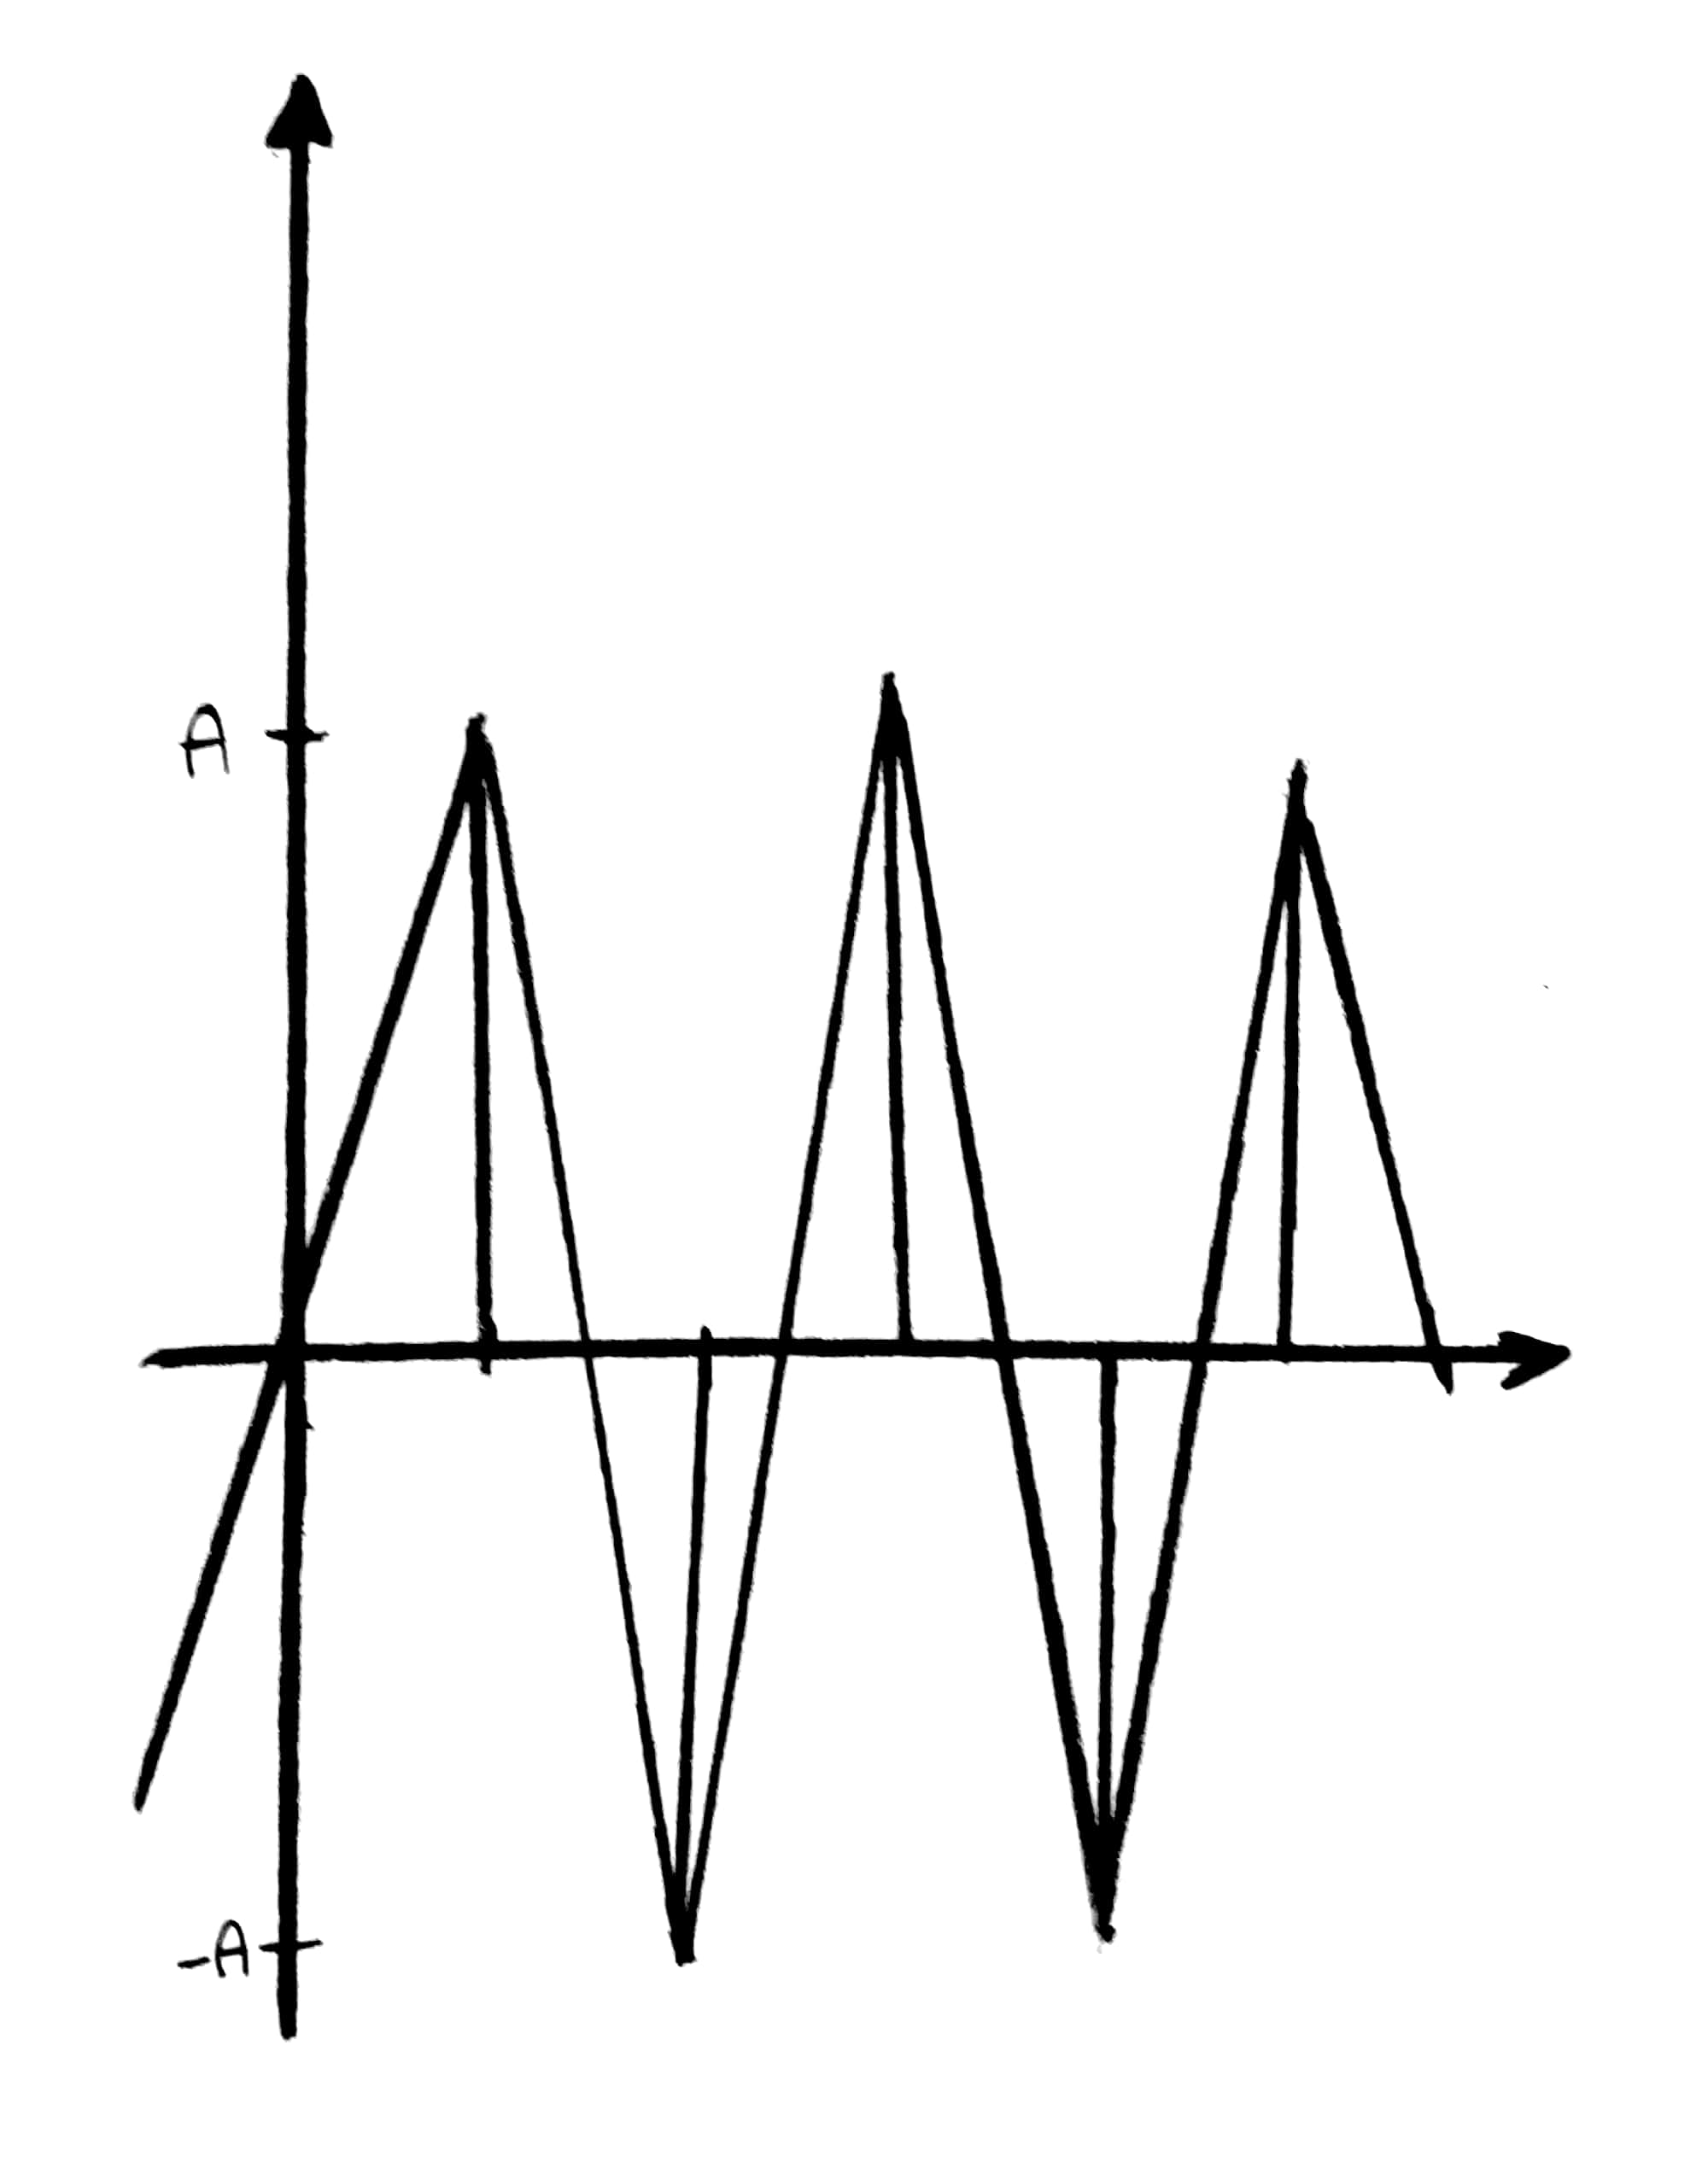
\includegraphics[width=0.35\textwidth]{SerieFourierEjemplo1}
                    \caption{Ve que es obvio que $\frac{a_0}{2}=0$}
                \end{figure}

                \begin{figure}[h]
                    \centering
                    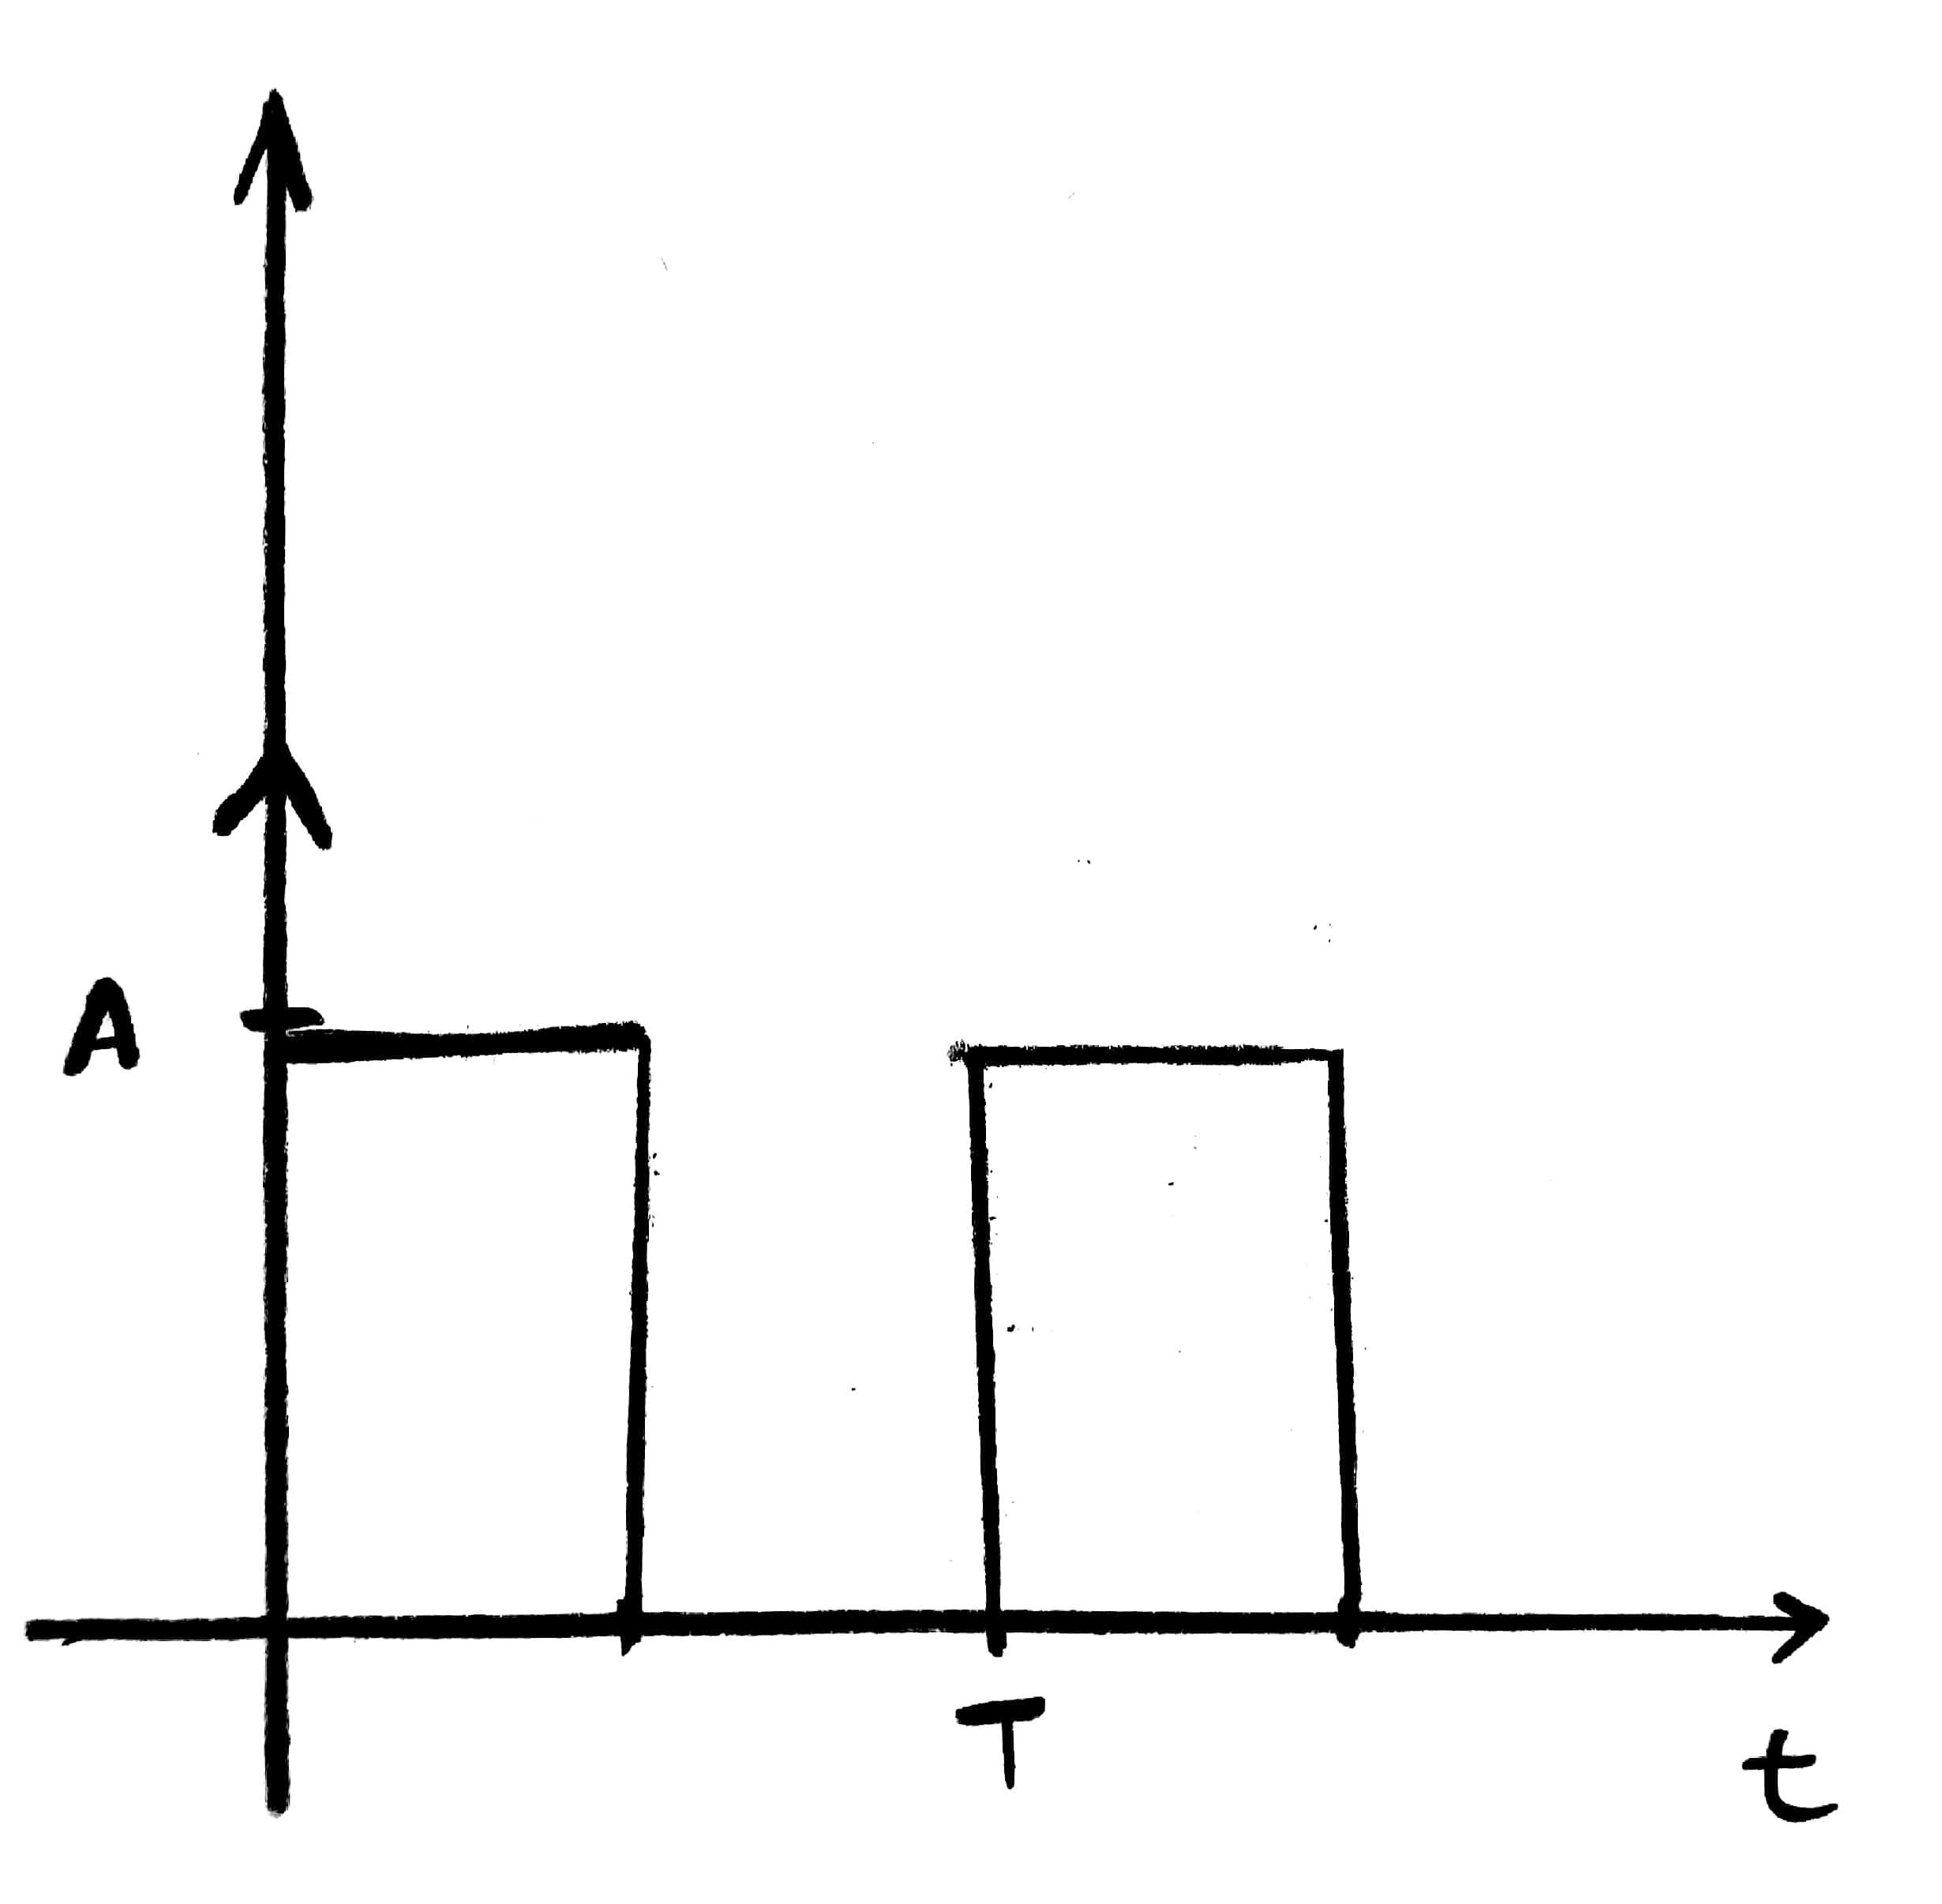
\includegraphics[width=0.35\textwidth]{SerieFourierEjemplo2}
                    \caption{Casi obvio que $\frac{a_0}{2}=\frac{A}{2}$}
                \end{figure}
                


            % ==========================
            % =======  a_n     =========
            % ==========================
            \clearpage
            \subsection{Encontrar a $a_n$}

                Sea $f(t)$ una función periódica y completamente IMPAR es decir $f(-t) = -f(t)$ entonces
                como es una función impar (tal y como el seno) espero que sea demasiado obvio que
                la expansión como serie de Fourier no tendrá SOLO elementos que involucren al seno
                (y quiza a $\dfrac{a_0}{2}$) entonces en resumen:

                \Quote{Si tu función es \textbf{impar} entonces $a_n = 0 \Space \forall n \in \Naturals$}



            % ==========================
            % =======  b_n     =========
            % ==========================
            \subsection{Encontrar a $b_n$}

                Sea $f(t)$ una función periódica y completamente PAR es decir $f(-t) = f(t)$ entonces
                como es una función par (tal y como el coseno) espero que sea demasiado obvio que
                la expansión como serie de Fourier no tendrá SOLO elementos que involucren al coseno
                (y quiza a $\dfrac{a_0}{2}$) entonces en resumen:

                \Quote{Si tu función es \textbf{par} entonces $b_n = 0 \Space \forall n \in \Naturals$}


        

        % ==============================================
        % ========   SERIE COMPLEJA DE FOURIER  ========
        % ==============================================
        \clearpage
        \section{Serie Compleja de Fourier}

            Creo que es más que obvio que $<e^{int}, e^{imt}$ son cero si y solo si $n=m$, por lo
            tanto podemos ver que son base, por lo tanto creo que es más que obvio que podemos
            expresar a la Serie de Fourier como:
            \begin{MultiLineEquation*}{3}
                f(t) = \dfrac{C_0}{2} + \sum_{n=1}^\infty C_n e^{inwt}
            \end{MultiLineEquation*}

            Calcular los coeficientes de dicha serie son casi una copia identica a los
            de la serie original y llegamos a:

            \begin{itemize}
                \item $C_0$:
                    \begin{MultiLineEquation*}{3}
                        \dfrac{C_0}{2} = \dfrac{1}{T}
                            \int_{\frac{-T}{2}}^{\frac{T}{2}} f(t) \; dt
                    \end{MultiLineEquation*}

                \item $C_n$:
                    \begin{MultiLineEquation*}{3}
                        C_n = \dfrac{1}{T}
                            \int_{\frac{-T}{2}}^{\frac{T}{2}} f(t) \; e^{-inwt}  \; dt
                    \end{MultiLineEquation*}
            \end{itemize}
                




        % ==============================================
        % ========     APLICACIONES DE SERIE    ========
        % ==============================================
        \clearpage
        \section{Aplicaciones - Problemas de Frontera}


            % ==============================================
            % ========    ECUACIONES DE ONDA        ========
            % ==============================================
            \subsection{Ecuación de Onda en una Dimensión}
                
                Consideremos una cuerda de longitud l, sujeta en sus extremos.

                Sea $u(x, t)$ una función que te cuenta el desplazamiento que
                sufre la cuerda en un tiempo t. Supongamos la posición 
                inicial esta dada por $f(x)$ y donde $c^2$ es una constante
                es $\frac{T}{p}$ donde $p$ es la razón de la masa de la cuerda
                entre unidad de longitud y $T$ es la tensión de la cuerda.

                Entonces:
                \begin{MultiLineEquation*}{3}
                    \UpperPartial{u(x, t)}{x}{2} 
                        &= \dfrac{1}{c^2} \; \UpperPartial{u(x, t)}{t}{2}
                \end{MultiLineEquation*}

                Veamos ahora algunas consideraciones (de frontera):
                \begin{itemize}
                    \item
                        $\forall t \; u(0, t) = u(l, t) = 0$. 
                        Porque la cuerda no se puede desplazar en los extremos
                    \item
                        $\forall t \; u(x, 0) = f(x)$. 
                        Porque literalmente así lo definimos tontito

                        $\Partial{u(x,t)}{t} \Evaluate_{t=0} = g(x)$
                \end{itemize}


                % ======== DEMOSTRACION ========
                \begin{SmallIndentation}[1em]
                    \textbf{Solución}:
                    
                    Ok, ok, esto va a ser largo, pero agarrate, veras que es
                    divertido. (Creo).

                    Supongamos que la solución de $u(x,t)$ es de la forma
                    $u(x,t) = X(t)T(t)$.

                    Es decir, la función que estamos buscando puede verse
                    como el producto de dos funciones que solo dependen de 
                    una variable.

                    Si esto fuera cierto, entonces tendremos que:
                    \begin{MultiLineEquation*}{3}
                        \UpperPartial{u(x, t)}{x}{2} = X''(x)T(t)
                        \Space\Space
                        \text{ y }
                        \Space\Space
                        \UpperPartial{u(x, t)}{t}{2} = X(x)T''(t)
                    \end{MultiLineEquation*}

                    Por lo tanto nuestra ecuación de la onda se ve como:
                    \begin{MultiLineEquation*}{3}
                        X''(x)T(t) = \dfrac{1}{c^2} \; X(x)T''(t)
                    \end{MultiLineEquation*}
                        

                    Ahora si separamos tenemos que:
                    \begin{MultiLineEquation*}{3}
                        \dfrac{X''(x)}{X(t)} = \dfrac{T''(t)}{c^2 T(t)}
                    \end{MultiLineEquation*}


                    \clearpage

                    Ahora viene lo interesante, ve que la parte a la izquierda
                    del igual es independiente de $t$ mientras que la parte
                    derecha de es independiente de $x$, ahora... ¿Cómo es 
                    posible que estas dos funciones sean iguales sin importar
                    cual es el valor de $x$ o de $t$?

                    Muy sencillo, si es que tanto $\dfrac{X''(x)}{X(t)}$ como
                    $\dfrac{T''(t)}{c^2 T(t)}$ es una constante.

                    Por lo tanto veamos que:
                    \begin{MultiLineEquation*}{3}
                        \dfrac{X''(x)}{X(t)} 
                            &= \dfrac{T''(t)}{c^2 T(t)}
                            &= -k^2
                    \end{MultiLineEquation*}
                        
                    Donde $-k^2$ es un constante, conocida como la constante
                    de separación.

                    Por lo tanto llegamos a dos ecuaciones diferenciales
                    lineales:
                    \begin{MultiLineEquation*}{3}
                        X''(x) + k^2 X(x)       = 0   \\
                        T''(x) + c^2k^2 T(t)    = 0   
                    \end{MultiLineEquation*}

                    Ahora, estas son ecuaciones que podemos solucionar,
                    de hecho su solución es un famosa:
                    \begin{MultiLineEquation*}{3}
                        X(x) = A\Cos{kx} + B\Sin{kx}    \\
                        T(t) = C\Cos{kct} + D\Sin{kct}
                    \end{MultiLineEquation*}

                    Ahora usemos las condiciones de frontera:

                    \begin{itemize}

                        \item 
                            Sabemos que $u(0,t)=X(0)T(t)=0$
                            por lo tanto como $t \neq 0$ entonces
                            $X(0)=0$

                        \item 
                            Sabemos que $u(l,t)=X(l)T(l)=0$
                            por lo tanto como $l \neq 0$ entonces
                            $X(l)=0$

                    \end{itemize}

                    De esto se muestra que:
                    \begin{MultiLineEquation*}{3}
                        X(0) &= A\Cos{0} + B\Sin{0}   
                             &= A
                             &= 0
                    \end{MultiLineEquation*}

                    Por otro lado con la segunda condición tenemos que 
                    \begin{MultiLineEquation*}{3}
                        X(t) &= B\Sin{kl}   
                             &= 0
                    \end{MultiLineEquation*}

                    Ahora, $B$ no puede ser cero, despues de todo si asi fuera
                    todo $u(x,t)$ sería siempre 0, así que solo nos queda
                    pensar en que $\Sin{kl}=0$, por lo tanto tenemos que:
                    $kl=n\pi$, es decir $k=\frac{n\pi}{l}$ donde $n$ podría ser
                    cualquier natural.

                    Por lo tanto la solución general es la suma de todas las
                    posibles soluciones, es decir:
                    \begin{MultiLineEquation*}{3}
                        u(x,t)
                            &= \sum_{n=1}^\infty u_n(x, t)
                            &= \sum_{n=1}^\infty
                                    \Sin{\frac{n \pi x}{l}}
                                    \Wrap{
                                        E_n \Cos{\frac{cn\pi t}{l}} +
                                        F_n \Sin{\frac{cn\pi t}{l}}
                                    }
                    \end{MultiLineEquation*}

                    \clearpage

                    Entonces sabemos que esta nueva forma de ver a $u(x,t)$
                    podemos ver las otras condiciones de otra manera
                    pues:

                    \begin{itemize}
                        
                        \item
                            $u(x,0)
                                = \displaystyle \sum_{n=1}^\infty
                                    E_n \Sin{\frac{n \pi x}{l}} = f(x)$

                            Por lo tanto $E_n$ son simplemente los coeficientes
                            de la expansión de la serie de Fourier, por lo 
                            tanto ya tenemos una forma de encontrar a los $E_n$
                            como:
                            \begin{MultiLineEquation*}{3}
                                E_n = \dfrac{2}{l} 
                                    \int_0^l f(x) \Sin{\frac{n \pi x}{l}} dx
                            \end{MultiLineEquation*}
                                


                        \item
                            $\Partial{u(x,t)}{t} \Evaluate_{t=0}
                                = \displaystyle\sum_{n=1}^\infty
                                    F_n \Sin{\frac{n \pi x}{l}} = g(x)$

                            Por lo tanto $F_n$ son simplemente los coeficientes
                            de la expansión de la serie de Fourier, por lo 
                            tanto ya tenemos una forma de encontrar a los $E_n$
                            como:
                            \begin{MultiLineEquation*}{3}
                                F_n = \dfrac{2}{cn\pi} 
                                    \int_0^l g(x) \Sin{\frac{n \pi x}{l}} dx
                            \end{MultiLineEquation*}


                    \end{itemize}
                        
                    Y por lo tanto, hemos encontrado una forma de 
                    encontrar a $u(x,t)$

                
                \end{SmallIndentation}






    % ===============================================================================
    % ===================        SERIES DE FOURIER          ==========================
    % ===============================================================================
    \chapter{Transformada de Fourier}
        \clearpage



        % ==============================================
        % ========     FUNCIONES ESPECIALES     ========
        % ==============================================
        \clearpage
        \section{Funciones Especiales}

            Tenemos dos funciones especiales que nos servirán mucho pronto


            % ==============================================
            % ========     FUNCIONES HEAVISIDE      ========
            % ==============================================
            \subsection{Función Heaviside - Escalón Unitario}
                \begin{MultiLineEquation*}{3}
                    H(t - a) =  \begin{cases}
                                    1 \Space & t \geq a \\ 
                                    0 \Space & t < a 
                                \end{cases}
                \end{MultiLineEquation*}

                \begin{itemize}
                    \item
                        Para filtrar $f(t)$ en el rango $[a,b]$
                        tenemos que hacer que:
                        \begin{MultiLineEquation*}{3}
                            f(t) [H(t-a) - H(t-b)]
                        \end{MultiLineEquation*}

                    \item
                        Para filtrar $[0,a]$
                        \begin{MultiLineEquation*}{3}
                            f(t) [H(t-a) H(t)]
                        \end{MultiLineEquation*}
                            
                            
                \end{itemize}



            % ==============================================
            % ========     FUNCIONES DELTA DE DIRAC ========
            % ==============================================
            \subsection{Función Delta de Dirac}

                Sea $\phi(x)$ una función de prueba, donde
                $\lim_{x \to \infty} \phi(x) = \lim_{x \to \infty} \phi(-x) = 0$

                \begin{itemize}
                    \item $\displaystyle \int_{-\infty}^\infty \delta(x) \; dx = 1$
                    \item $\displaystyle \int_{-\infty}^\infty \phi(x) \delta(x) \; dx = \phi(0)$
                    \item $\displaystyle \int_{-\infty}^\infty \phi(x) \delta(x-x_0) \; dx = \phi(x_0)$
                    \item $\displaystyle \int_{-\infty}^\infty \phi'(x) \delta(x)  \; dx =
                           \displaystyle \int_{-\infty}^\infty \phi(x)  \delta'(x) \; dx = \phi'(0)$
                \end{itemize}
                    



        % ==============================================
        % == DEFINICIÓN DE LA TRANSFORMADA DE FOURIER ==
        % ==============================================
        \clearpage
        \section{Definición}

            Sea $f(t)$ una función periódica tal que $\int_{-\infty}^\infty |f(t)| dt < \infty$
            entonces podemos definir a la transformada de Fourier como:
            \begin{MultiLineEquation*}{3}
                \FourierT{f(t)} = \int_{-\infty}^\infty f(t) \; e^{-iwt} \; dt
            \end{MultiLineEquation*}

            Es decir:
            \begin{itemize}
                \item $f(t)$ es una función que definimos en el tiempo
                \item $\FourierT{f(t)}$ ó $F(w)$ es una función en el espacio de la frecuencia
                \item Diremos que para una función genérica su transformada esta denotada por $F(w)$
            \end{itemize}



            % ======================================
            % ========       PROPIEDADES    ========
            % ======================================
            \subsection{Propiedades}

                \begin{itemize}
                    \item
                        Recuerda la función a la cual le quieras aplicar una Transformada de Fourier
                        tu función tiene que converger, es decir $\int_{-\infty}^\infty |f(t)| dt < \infty$

                    \item
                        La Transformada es una \Quote{función lineal}, es decir:\\
                        $\FourierT{a[f(t)] + b[g(t)]} = a\FourierT{f(t)} + b\FourierT{g(t)}$

                    \item 
                        La Transformada es un isomorfismo, es decir, es lo que llamaríamos una \Quote{función
                        biyectiva} por lo tanto podemos hablar de la Transformada inversa.
                \end{itemize}


        % ==============================================
        % = TRANSFORMADA - INTEGRAL COMPLEJA FOURIER   =
        % ==============================================
        \clearpage
        \section{Transformada y la Integral Compleja de Fourier}

            En este texto no hablamos mucho de la integral compleja de Fourier, pero 
            existe una relación bastante interesante entre los mismo, podemos decir que:

            Sea $f(t)$ una función que tenga una Transformada de Fourier, denotada por $F(w)$
            entonces podemos decir que la integral compleja de Fourier como:
            \begin{MultiLineEquation*}{3}
                f(t) = \dfrac{1}{2\pi} \int_{-\infty}^{\infty} F(w) e^{wit} \; dt
            \end{MultiLineEquation*}

            Si te das cuenta esta forma de escribir a $f(t)$ es una forma de definir a la transformada 
            inversa.



        % ==============================================
        % =====    TRANSFORMADA MAS FAMOSAS      =======
        % ==============================================
        \clearpage
        \section{Transformadas por Definición}


            % ==============================================
            % =====    TRANSFORMADA MAS FAMOSAS      =======
            % ==============================================
            \subsection{$\FourierT{e^{-\alpha t}}$}

                A ver, a ver, antes de que te me enojes, $e^{-\alpha t}$ no converge, solo converge
                la parte positiva, por lo tanto, más bien sacaremos la Transformada de $e^{-\alpha t}$ cuando
                $t \geq 0$.
                \begin{MultiLineEquation*}{3}
                    \FourierT{e^{-\alpha t}}
                        &= \int_{-\infty}^\infty u(t) e^{-\alpha t} \; e^{-iwt} \; dt       \\
                        &= \int_0^\infty e^{-\alpha t} \; e^{-iwt} \; dt                    \\
                        &= \int_0^\infty e^{-(iw + \alpha)t} \; dt                          \\
                        &= \pfrac{1}{iw+\alpha} e^{-(iw + \alpha)t} \Evaluate_0^\infty      \\
                        &= \dfrac{1}{iw+\alpha}                               
                \end{MultiLineEquation*}



            % ==============================================
            % =====    TRANSFORMADA MAS FAMOSAS      =======
            % ==============================================
            \subsection{$\FourierT{k}$}

                A ver, a ver, antes de que te me enojes, $f(t) = k$ no converge, solo converge
                si es que tomamos a $f(t) = k$ en un rango, un rango de longitud $d$, osea desde
                $\frac{-d}{2}$ hasta $\frac{d}{2}$ y $f(t) = 0$ en todos los otros lados.
                \begin{MultiLineEquation*}{3}
                    \FourierT{k[u(t+\tfrac{d}{2}) - u(t-\tfrac{d}{2})]}
                        &= \int_{-\infty}^\infty k[u(t+\tfrac{d}{2}) - u(t-\tfrac{d}{2})] \; e^{-iwt} \; dt   \\
                        &= k\int_{-\infty}^\infty u(t+\tfrac{d}{2}) - u(t-\tfrac{d}{2}) \; e^{-iwt} \; dt     \\
                        &= k\int_{-\frac{d}{2}}^{\frac{d}{2}}  e^{-iwt} \; dt                               \\
                        &= \dfrac{k}{iw} e^{-iwt} \Evaluate_{-\frac{d}{2}}^{\frac{d}{2}}                    \\
                        &= \dfrac{2k}{w} \Sin{\dfrac{wd}{2}}                             
                \end{MultiLineEquation*}


            % ==============================================
            % =====    TRANSFORMADA MAS FAMOSAS      =======
            % ==============================================
            \subsection{$\FourierT{\delta(t)}$}

                Recuerda lo que vimos hace unas páginas, porque vamos a usar que
                $\int_{-\infty}^\infty \delta(t) f(t) = f(0)$
                \begin{MultiLineEquation*}{3}
                    \FourierT{\delta(t)}
                        &= \int_{-\infty}^\infty \delta(t) \; e^{-iwt} \; dt   \\
                        &= e^{-iw(0)}                                          \\
                        &= 1
                \end{MultiLineEquation*}
                    




        % ==============================================
        % =====    TRANSFORMADA MAS FAMOSAS      =======
        % ==============================================
        \clearpage
        \section{Teoremas de la Derivadas}

            % ==============================================
            % =====    DERIVADAS EN LA FRECUENCIA    =======
            % ==============================================
            \subsection{Derivada con Respecto a la Frecuencia}
                Esta es de las importantes
                \begin{MultiLineEquation*}{3}
                    \UpperDerivate{F(w)}{w}{n}
                        &= \MiniUpperDerivate{w}{n} \int_{-\infty}^\infty f(t)  \; e^{-iwt} \; dt     \\
                        &= \int_{-\infty}^\infty f(t)  \; \UpperPartial{e^{-iwt}}{w}{n} dt            \\
                        &= \int_{-\infty}^\infty f(t)  \; (-it)^n e^{-iwt} dt                         \\
                        &= \FourierT{f(t) t^n i^{-n}}
                \end{MultiLineEquation*}

                Por lo tanto tienes que:
                \begin{MultiLineEquation*}{3}
                    \FourierT{t^n f(t)} = i^n \UpperDerivate{F(w)}{w}{n}
                \end{MultiLineEquation*}

            % ==============================================
            % =====    DERIVADAS EN EL TIEMPO        =======
            % ==============================================
            \subsection{Derivada con Respecto al Tiempo}

                De una manera similar podemos decir que:
                \begin{MultiLineEquation*}{3}
                    \FourierT{\UpperDerivate{f(x)}{x}{n}} = (iw)^n F(w)
                \end{MultiLineEquation*}





        % ==============================================
        % =========    DESPLAZAMIENTOS     =============
        % ==============================================
        \clearpage
        \section{Desplazamientos}

            % ==============================================
            % =====    DESPLAZAMIENTO EN EL TIEMPO    ======
            % ==============================================
            \subsection{Desplazamiento en Tiempo}

                Se conoce también como la propiedad de Corrimiento de Tiempo y nos permite
                calcular la Transformada de Fourier de una función $f(t)$ que esta desplazada
                sobre $t$.
                \begin{MultiLineEquation*}{3}
                    \FourierT{f(t-t_0)} = e^{-iwt_0} F(w)
                \end{MultiLineEquation*}


                % ======== DEMOSTRACION ========
                \begin{SmallIndentation}[1em]
                    \textbf{Demostración}:
                    
                    Basta con ver que pasa al momento de calcular la transformada de $f(t - t_0)$
                    \begin{MultiLineEquation*}{3}
                        \FourierT{e^{iw_0 t} f(t)} 
                            &= \int_{-\infty}^\infty f(t - t_0) \; e^{-iwt} dt                          \\
                            &= \int_{-\infty}^\infty f(t - t_0) \; e^{-iwt} e^{+iwt_0} e^{-iwt_0} dt    \\
                            &= e^{-iwt_0} \int_{-\infty}^\infty f(t - t_0) \; e^{-iw(t - t_0)}  dt      \\
                            &= e^{-iwt_0} \int_{-\infty}^\infty f(u) \; e^{-iw(u)}  du                  \\
                            &= e^{-iwt_0} F(w)
                    \end{MultiLineEquation*}
                        
                
                \end{SmallIndentation}


                % ==============================================
                % =====    EJEMPLOS DE TRANSFORMADAS     =======
                % ==============================================
                \clearpage
                \subsection{Ejemplos de Desplamiento de Tiempo}

                    % =================================
                    % ========     EJEMPLO  ===========
                    % =================================
                    \subsubsection{Ejemplo 1}

                        Sea $f(t) = \begin{cases}
                                        5 \in [4, 10]       \\
                                        0 \notin [4, 10]    \\
                                    \end{cases}$

                        Calcular $\FourierT{f(t)}$

                        % ======== DEMOSTRACION ========
                        \begin{SmallIndentation}[1em]
                            \textbf{Solución}:

                            Empecemos por la idea de que es una función que esta corrida en el tiempo, por lo tanto
                            pensemos en la misma función, pero centrada en el origen.

                            De esto sabemos que $\FourierT{5[u(t+3) - u(t-3]} = \dfrac{10}{w} \Sin{3w}$, por lo 
                            tanto simplemente tenemos que correrla en el tiempo, por lo tanto:

                            $\FourierT{5[u(t-4) - u(t-10]} = \dfrac{10e^{7iw}}{w} \Sin{3w}$

                        \end{SmallIndentation}


                    % =================================
                    % ========     EJEMPLO  ===========
                    % =================================
                    \subsubsection{Ejemplo 2}

                        Sea $f(t) = 5[u(t-3) -u(t-11)]$

                        Calcular $\FourierT{f(t)}$

                        % ======== DEMOSTRACION ========
                        \begin{SmallIndentation}[1em]
                            \textbf{Solución}:

                            Primero empecemos por pensar que esta corrida 7 unidades, la original
                            sería $g(t) = f(t+7) = 5[u(t+4)-u(t-4)]$, por lo tanto $G(w)$ es simplemente
                            $\dfrac{10}{w} \Sin{4w}$, por lo tanto:

                            \begin{MultiLineEquation*}{3}
                                F(w)
                                    &= \FourierT{g(t)} = \FourierT{f(t+7)}  \\
                                    &= e^{-iw(-7)} \dfrac{10}{w} \Sin{4w}   \\
                                    &= e^{7iw} \dfrac{10}{w} \Sin{4w}       
                            \end{MultiLineEquation*}

                        \end{SmallIndentation}


                    % =================================
                    % ========     EJEMPLO  ===========
                    % =================================
                    \clearpage
                    \subsubsection{Ejemplo 3}

                        Sea $f(t) =u(t-2) e^{-3t}$

                        Calcular $\FourierT{f(t)}$

                        % ======== DEMOSTRACION ========
                        \begin{SmallIndentation}[1em]
                            \textbf{Solución}:

                            Veamos

                            \begin{MultiLineEquation*}{3}
                                \FourierT{f(t+7)} 
                                    &= \FourierT{u(t-2) \Wrap{e^{-3(t-2)}}e^{-6}}      
                                        && \Remember{Recuerda que $e^{-6}$ es un número}    \\
                                    &= e^{-6}\FourierT{u(t-2) e^{-3(t-2)}}      
                                        && \Remember{Por lo tanto podemos sacarlo}          \\
                                    &= e^{-6} \; e^{-2iw} \FourierT{u(t)e^{-3t}}      
                                        && \Remember{Esta corrido en el tiempo}             \\
                                    &= e^{-6} \; e^{-2iw} \dfrac{1}{3+iw}      
                                        && \Remember{Magia ... casi}                        \\
                                    &= \dfrac{e^{-(2iw + 6)}}{3+iw}      
                                        && \Remember{Magia} 
                            \end{MultiLineEquation*}

                        \end{SmallIndentation}


                    % =================================
                    % ========     EJEMPLO  ===========
                    % =================================
                    \subsubsection{Ejemplo 4}

                        Sea $f(t) = 5 e^{-3(t-5)^2}$

                        Calcular $\FourierT{f(t)}$

                        % ======== DEMOSTRACION ========
                        \begin{SmallIndentation}[1em]
                            \textbf{Solución}:
                            \begin{MultiLineEquation*}{3}
                                F(w)
                                    &= \FourierT{5 e^{-3(t-5)^2}}                               \\
                                    &= 5 \FourierT{e^{-3(t-5)^2}}          
                                        && \Remember{Recuerda que es lineal}                    \\
                                    &= 5 e^{-5iw} \FourierT{e^{-3t^2}}          
                                        && \Remember{Estaba corrida en el tiempo}               \\
                                    &= 5 e^{-5iw} \Wrap{
                                            \sqrt{\frac{\pi}{3}} e^{-\frac{w^2}{12}} 
                                        }         
                                        && \Remember{Ahora si aplicamos una directa}            \\
                                    &= \frac{5\pi}{3} e^{-(5iw + \frac{w^2}{12})}
                                        && \Remember{Magia}           
                            \end{MultiLineEquation*}

                        \end{SmallIndentation}


            % ==============================================
            % ===  DESPLAZAMIENTO EN EL FRECUENCIA     =====
            % ==============================================
            \clearpage
            \subsection{Desplazamiento en Frecuencia}

                Se conoce también como la propiedad de Corrimiento de Frecuencia y nos permite
                encontrar la Transformada de Fourier de una función sabiendo $F(w)$
                \begin{MultiLineEquation*}{3}
                    \FourierT{e^{iw_0 t} \; f(t)} = F(w - w_0) 
                \end{MultiLineEquation*}

                % ======== DEMOSTRACION ========
                \begin{SmallIndentation}[1em]
                    \textbf{Demostración}:
                    
                    Basta con ver que pasa al momento de calcular la transformada de $e^{iw_0 t} \; f(t)$
                    \begin{MultiLineEquation*}{3}
                        \FourierT{e^{iw_0 t} f(t)} 
                            &= \int_{-\infty}^\infty e^{iw_0 t} f(t) \; e^{-iw t} dt        \\
                            &= \int_{-\infty}^\infty e^{-i(w - w_0)t} f(t) dt               \\
                            &= \int_{-\infty}^\infty f(t) e^{-i(w - w_0)t} dt               \\
                            &= F(w - w_0)
                    \end{MultiLineEquation*}
                        
                
                \end{SmallIndentation}
                    

                
        % ==============================================
        % =====    TRANSFORMADA MAS FAMOSAS      =======
        % ==============================================
        \clearpage
        \section{Gran Teorema de la Simetría}

            Esta es la propiedad más importante que verás en todos estos archivos de Fourier,
            es fácil de escribir pero algo más complicado de explicar.

            Sea $\FourierT {f(t)} = F(w)$, entonces:
            \begin{MultiLineEquation*}{3}
                \FourierT{F(t)} = 2 \pi \; f(-w)
            \end{MultiLineEquation*}

            Es decir, la transformada de $F(t)$, es decir de una función que se parece mucho
            a la transformada de $f(t)$ osea $F(w)$ pero no en el dominio de la frecuencia sino
            en el dominio del tiempo es igual a $2\pi$ por $f(-w)$ donde $f(w)$ es algo parecido
            a $f(t)$ pero en el dominio de la frecuencia.


   
            % ==============================================
            % =====    TRANSFORMADA MAS FAMOSAS      =======
            % ==============================================
            \subsection{Consecuencia: $\FourierT{1}$}

                Usando que $\FourierT{\delta(t)} = 1$ podemos decir que:\\
                $\FourierT{1} = 2\pi \delta(-w)$




        % ==============================================
        % =====    TRANSFORMADA MAS FAMOSAS      =======
        % ==============================================
        \clearpage
        \section{Teorema del Escalamiento}

            Si para una función $f(t)$ existe su Transformada de Fourier, entonces podemos decir
            que:
            \begin{MultiLineEquation*}{3}
                \FourierT{f(at)} = \frac{1}{|a|} \; F\Wrap{\frac{w}{a}}
            \end{MultiLineEquation*}

            % ======== DEMOSTRACION ========
            \begin{SmallIndentation}[1em]
                \textbf{Demostración}:
                
                Basta con ver que pasa al momento de calcular la transformada de $f(at)$,
                eso si antes sea $r=at$ y $dt = \frac{dr}{a}$
                \begin{MultiLineEquation*}{3}
                    \FourierT{e^{iw_0 t} f(t)} 
                        &= \int_{-\infty}^\infty f(at) \; e^{-iw t} dt                          \\
                        &= \int_{-\infty}^\infty f(r) \; e^{-iw \frac{r}{a}} \dfrac{dr}{a}      \\
                        &= \dfrac{1}{|a|} \int_{-\infty}^\infty f(r) \; e^{-i \frac{w}{a} r} dr \\
                        &= \dfrac{1}{|a|} F\Wrap{\frac{w}{a}}
                \end{MultiLineEquation*}
            
            \end{SmallIndentation}


            % ==============================================
            % =====    CONSECUENCIA DE SIMETRIA      =======
            % ==============================================
            \subsection{Consecuencia: Inverte el Tiempo $\FourierT{f(-t)}$}


                Esto es una consecuencia directa del teorema anterior, pero es tan interesante que
                le daré su propio espacio:
                \begin{MultiLineEquation*}{3}
                    \FourierT{f(-t)} = F(-w)
                \end{MultiLineEquation*}

                % ======== DEMOSTRACION ========
                \begin{SmallIndentation}[1em]
                    \textbf{Demostración}:
                    
                    Usando el Teorema del Escalamiento podemos pensar en $a = -1$, entonces
                    basta con ver que:
                    \begin{MultiLineEquation*}{3}
                        \FourierT{f((-1)t)} 
                            &= \FourierT{f(-t)}                             \\
                            &= \frac{1}{|-1|} \; F\Wrap{\frac{w}{-1}}       \\
                            &= \frac{1}{1} \; F(-w)                         \\
                            &= F(-w)
                    \end{MultiLineEquation*}
                
                \end{SmallIndentation}


            % ==============================================
            % =====    CONSECUENCIA DE SIMETRIA      =======
            % ==============================================
            \subsection{Consecuencia: Una Clásica $\FourierT{e^{-a|t|}}$}

                Esto es una consecuencia directa del teorema anterior, pero es tan interesante que
                le daré su propio espacio:
                \begin{MultiLineEquation*}{3}
                   \FourierT{e^{-a|t|}} = \frac{2a}{a^2 + w^2}
                \end{MultiLineEquation*}

                % ======== DEMOSTRACION ========
                \begin{SmallIndentation}[1em]
                    \textbf{Demostración}:
                    
                    El truco esta en ver las diferentes formas en que podemos ver a 
                    $e^{-a|t|}$.

                    \begin{MultiLineEquation*}{3}
                        \FourierT{e^{-a|t|}}
                            &= \FourierT{u(t) e^{-at} + u(-t) e^{at} }
                                && \Remember{Dos funciones, una para los negativos otra positivos}  \\
                            &= \FourierT{f(t) + f(-t) }
                                && \Remember{Paso Clave, sea $f(t)=u(t)e^{-at}$}                    \\
                            &= \FourierT{f(t)} + \FourierT{f(-t)}
                                && \Remember{Separamos}                                             \\
                            &= F(w) + F(-w)
                                && \Remember{Aplicamos inverso del tiempo}                          \\
                            &= \frac{1}{a + iw} + \frac{1}{a - iw}
                                && \Remember{Son transformadas directas si sabes $f(t)$}            \\
                            &= \frac{(a + iw) + (a - iw)}{(a + iw)(a - iw)}
                                && \Remember{Sumamos las 2 fracciones}                              \\
                            &= \frac{2a}{a^2 - (iw)^2}
                                && \Remember{Diferencia de Cuadrados}                               \\
                            &= \frac{2a}{a^2 + w^2}
                                && \Remember{Magia}
                    \end{MultiLineEquation*}

                
                \end{SmallIndentation}
                    




        % ==============================================
        % =====    TEOREMA DE LA MODULACIÓN      =======
        % ==============================================
        \clearpage
        \section{Teoremas de la Modulación}

            % ==============================================
            % =====    TRANSFORMADA MAS FAMOSAS      =======
            % ==============================================
            \subsection{$\FourierT{f(t) \; \Cos{w_0t}}$}

                Seguro que esta tiene nombre pero ni idea :/
                \begin{MultiLineEquation*}{3}
                    \FourierT{f(t) \; \Cos{w_0t}}
                        &= \int_{-\infty}^\infty f(t) \Cos{w_0t} \; e^{-iwt} \; dt                      \\
                        &= \int_{-\infty}^\infty f(t) \pfrac{e^{w_0t}+e^{-w_0t}}{2} \; e^{-iwt} \; dt   \\
                        &= \dfrac{1}{2} \int_{-\infty}^\infty f(t) e^{-i(w-w_0)} dt
                                +
                           \dfrac{1}{2} \int_{-\infty}^\infty f(t) e^{-i(w+w_0)} dt                     \\
                        &= \dfrac{1}{2}\Brackets{F(w-w_0) + F(w+w_0)}
                \end{MultiLineEquation*}


            % ==============================================
            % =====    TRANSFORMADA MAS FAMOSAS      =======
            % ==============================================
            \subsection{$\FourierT{\Cos{w_0t}}$}

                Usando lo anterior:
                \begin{MultiLineEquation*}{3}
                    \FourierT{\Cos{w_0t}}
                        &= \int_{-\infty}^\infty 1 \Cos{w_0t} \; e^{-iwt} \; dt             \\
                        &= \dfrac{1}{2}\Brackets{2\pi \delta(-w-w_0) + 2\pi\delta(-w+w_0)}  \\
                        &= \pi \delta(-w-w_0) + \pi \delta(-w+w_0)                          \\
                        &= \pi (\delta(-w-w_0) + \delta(-w+w_0))
                \end{MultiLineEquation*}


            \clearpage                    


            % ==============================================
            % =====    TRANSFORMADA MAS FAMOSAS      =======
            % ==============================================
            \subsection{$\FourierT{f(t) \; \Sin{w_0t}}$}

                Seguro que esta tiene nombre pero ni idea :/
                \begin{MultiLineEquation*}{3}
                    \FourierT{f(t) \; \Sin{w_0t}}
                        &= \int_{-\infty}^\infty f(t) \Cos{w_0t} \; e^{-iwt} \; dt                      \\
                        &= \int_{-\infty}^\infty f(t) \pfrac{e^{w_0t}-e^{-w_0t}}{2i} \; e^{-iwt} \; dt  \\
                        &= \dfrac{1}{2i} \int_{-\infty}^\infty f(t) e^{-i(w-w_0)} dt
                                -
                           \dfrac{1}{2i} \int_{-\infty}^\infty f(t) e^{-i(w+w_0)} dt                     \\
                        &= \dfrac{1}{2i}\Brackets{F(w-w_0) - F(w+w_0)}                                   \\
                        &= 2i\Brackets{F(w+w_0) - F(w-w_0)}
                \end{MultiLineEquation*}

            % ==============================================
            % =====    TRANSFORMADA MAS FAMOSAS      =======
            % ==============================================
            \subsection{$\FourierT{\Sin{w_0t}}$}

                Usando lo anterior:
                \begin{MultiLineEquation*}{3}
                    \FourierT{\Cos{w_0t}}
                        &= \int_{-\infty}^\infty 1 \Sin{w_0t} \; e^{-iwt} \; dt             \\
                        &= \dfrac{1}{2i}\Brackets{2\pi \delta(-w-w_0) - 2\pi\delta(-w+w_0)} \\
                        &= -i\pi \delta(-w-w_0) + i\pi(-w+w_0)                              \\
                        &= i\pi\delta(-w+w_0) - i\pi \delta(-w-w_0)
                \end{MultiLineEquation*}





            % ==============================================
            % =====    EJEMPLOS DE TRANSFORMADAS     =======
            % ==============================================
            \clearpage
            \subsection{Ejemplos}

                % =================================
                % ========     EJEMPLO  ===========
                % =================================
                \subsubsection{Ejemplo 1}

                    Sea $f(t) = 5\dfrac{\Sin{t}}{t}$

                    Calcular $\FourierT{f(t)}$

                    % ======== DEMOSTRACION ========
                    \begin{SmallIndentation}[1em]
                        \textbf{Solución}:

                        Veamos, pero antes de empezar con las cuentas
                        tienes que ver que $g(t) = \dfrac{1}{2}[u(t-1) - u(t+1)]$ y por lo
                        tanto $G(w) = \dfrac{1}{w} \Sin{w}$

                        \begin{MultiLineEquation*}{3}
                            \FourierT{f(t)} 
                                &= \FourierT{5\dfrac{\Sin{t}}{t}}      
                                    && \Remember{Empecemos}                                 \\
                                &= 5\FourierT{\dfrac{\Sin{t}}{t}}      
                                    && \Remember{La Transformada es lineal ;)}              \\
                                &= 10 \pi \Wrap{\dfrac{1}{2}[u(t-1) - u(t+1)]} \Evaluate_{-w}      
                                    && \Remember{Mira lo que esta hasta arriba, simetria}   \\
                                &= 5 \pi [u(-w-1) - u(-w+1)]
                        \end{MultiLineEquation*}

                    \end{SmallIndentation}



                % =================================
                % ========     EJEMPLO  ===========
                % =================================
                \subsubsection{Ejemplo 2}

                    Sea $f(t) = 4 u(t-2) e^{-3t} \Cos{t-2}$

                    Calcular $\FourierT{f(t)}$

                    % ======== DEMOSTRACION ========
                    \begin{SmallIndentation}[1em]
                        \textbf{Solución}:
                        \begin{MultiLineEquation*}{3}
                            F(w)
                                &= \FourierT{4 u(t-2) e^{-3t} \Cos{t-2}}                    \\
                                &= 4 \FourierT{u(t-2) e^{-3(t-2)} e^{-6} \Cos{t-2}}          
                                    && \Remember{Recuerda que es lineal}                    \\
                                &= 4e^{-6} \FourierT{u(t-2) e^{-3(t-2)} \Cos{t-2}}          
                                    && \Remember{Recuerda que es lineal}                    \\
                                &= 4e^{-6} e^{-2iw} \; \FourierT{u(t) e^{-3t} \Cos{t} }          
                                    && \Remember{Estaba corrida en el tiempo}               \\
                                &= 4e^{-(2iw+6)} \pfrac{1}{2}\Wrap{
                                        \frac{1}{3 + i(w-1)} + \frac{1}{3 + i(w+1)} 
                                    }         
                                    && \Remember{Ahora si aplicamos una directa}            \\
                                &= 2e^{-(2iw+6)}
                                    \Wrap{
                                        \frac{1}{3 + i(w-1)} + \frac{1}{3 + i(w+1)} 
                                    }
                                    && \Remember{Magia}           
                        \end{MultiLineEquation*}

                    \end{SmallIndentation}






        % ===============================================
        % =====       TRANSFORMADA INVERSA        =======
        % ===============================================
        \clearpage
        \section{Transformada Inversa}

            Ya que tenemos una linda forma de encontrar la transformada de Fourier también podemos
            hacer algo parecido con la transformada inversa y definirla como:
            \begin{MultiLineEquation*}{3}
                f(t) = \dfrac{1}{2\pi} \int_{-\infty}^\infty F(w) e^{iw t} dw
            \end{MultiLineEquation*}
                

            % ===============================================
            % =====       EJEMPLOS DE INVERSAS        =======
            % ===============================================
            \clearpage
            \subsection{Ejemplos de la Inversa}

                % =================================
                % ========     EJEMPLO  ===========
                % =================================
                \subsection*{Ejemplo 1}

                    Calcula $\InvFourierT{\dfrac{4e^{(2w-6)i}}{5-(3-w)i}}$

                    % ======== DEMOSTRACION ========
                    \begin{SmallIndentation}[1em]
                        \textbf{Solución}:
                        
                        Esto va a esta bien intenso, pero bien genial, veamos:
                        \begin{MultiLineEquation*}{3}
                            \InvFourierT{\dfrac{4e^{(2w-6)i}}{5-(3-w)i}}
                                &= \InvFourierT{\dfrac{4e^{2(w-3)i}}{5+(w-3)i}}     
                                    && \Remember{Arreglamos los términos}                                \\
                                &= e^{i3t} \InvFourierT{\dfrac{4e^{2wi}}{5+wi}}     
                                    && \Remember{Estaba movida}                                          \\
                                &= 4e^{i3t} \InvFourierT{\dfrac{e^{2wi}}{5+wi}}     
                                    && \Remember{La Transformada (y si inversa el lineal)}               \\
                                &= 4e^{i3t} \InvFourierT{\dfrac{1}{5+wi}} \Evaluate_{t=t+2}     
                                    && \Remember{También estaba corrida}                                 \\
                                &= 4e^{i3t} \Wrap{u(t)e^{-5t}}\Evaluate_{t=t+2}     
                                    && \Remember{Nos sabemos la Transformada de esa}                     \\
                                &= 4e^{i3t} \; u(t+2)e^{-5(t+2)}     
                                    && \Remember{Magia :D}                                             
                        \end{MultiLineEquation*}
                            
                    
                    \end{SmallIndentation}
                        


                % =================================
                % ========     EJEMPLO  ===========
                % =================================
                \subsubsection{Ejemplo 2}

                    Encuentra $\InvFourierT{\frac{1+iw}{(2+iw)(3+iw)}}$

                    % ======== DEMOSTRACION ========
                    \begin{SmallIndentation}[1em]
                        \textbf{Solución Forma Inteligente}:
                        \begin{MultiLineEquation*}{3}
                            f(t)
                                &= \InvFourierT{\frac{1+iw}{(2+iw)(3+iw)}}                            
                                    && \Remember{Piensa}                                                    \\
                                &= \InvFourierT{\frac{-1}{(2+iw)} + \frac{2}{(3+iw)}}                          
                                    && \Remember{Ahi esta el truco}                                         \\
                                &= \InvFourierT{\frac{-1}{(2+iw)}} + \InvFourierT{\frac{2}{(3+iw)}}         
                                    && \Remember{Ahora la puedo separar}                                    \\
                                &= -u(t)e^{-2t} + 2u(t)e^{-3t}
                                    && \Remember{Ahora la puedo separar}                                    \\
                                &= u(t)[2e^{-3t} - e^{-2t}]
                                    && \Remember{Ahora reparo y pongo bonito}                                    
                        \end{MultiLineEquation*}

                    \end{SmallIndentation}




        % ===============================================
        % ========       CONVOLUCION              =======
        % ===============================================
        \clearpage
        \section{Convolución}

            Si tenemos dos funciones $f(t)$, $g(t)$ tienen su transformada de Fourier
            entonces podemos hablar de la Convolución.
            \begin{MultiLineEquation*}{3}
                f(t) * g(t) = \int_{-\infty}^\infty f(t-x) \; g(x) dx
            \end{MultiLineEquation*}

            Además tenemos una propiedad muy importante:
            \begin{MultiLineEquation*}{3}
                \FourierT{f(t) \;*\; g(t)} = F(w) \; G(w)
            \end{MultiLineEquation*}

            Nota que la definición de Convolución no depende de nada de Fourier, por lo tanto
            esta definición aplica para todas las transformadas.


                % ==================================
                % =======      PROPIEDADES   =======
                % ==================================
                \subsection{Propiedades}

                    \begin{itemize}
                        \item La Convolución es conmutativa, es decir $f * g = g * f$
                        \item La Convolución es lineal, es decir $(af + bg)*h = a(f*h) + b(g*h)$
                    \end{itemize}



                % ==================================
                % =====    EJEMPLO           =======
                % ==================================
                \clearpage
                \subsection{Ejemplos usando Convolución para la Inversa}

                    % =================================
                    % ========     EJEMPLO  ===========
                    % =================================
                    \subsubsection{Ejemplo 1}

                    Encuentra $\InvFourierT{\frac{1}{(1+iw)^2}}$

                    % ======== DEMOSTRACION ========
                    \begin{SmallIndentation}[1em]
                        \textbf{Solución Forma 1}:
                        
                        Ve que $\MiniDerivate[w] \frac{1}{(1+iw)^2} = \frac{-i}{(1+iw)^2}$
                        y si multiplicas todo por $i$ tienes que 
                        $i \MiniDerivate[w] \frac{1}{(1+iw)^2} = \frac{1}{(1+iw)^2}$

                        Por lo tanto creo que es muy obvio usando el Teorema de la Derivación que:\\
                        $\InvFourierT{\frac{1}{(1+iw)^2}} = t \; u(t) \; e^{-t}$.

                        Y bingo, hemos acabado.

                        \vspace{3em}

                        \textbf{Solución Forma 2}:

                        Pero usando Convolución:
                        \begin{MultiLineEquation*}{3}
                            \InvFourierT{\frac{1}{(1+iw)^2}}
                                &= \InvFourierT{\frac{1}{(1+iw)} \frac{1}{(1+iw)}}                   \\
                                &= u(t) e^{-t} * u(t) e^{-t}                                         \\
                                &= \int_{-\infty}^\infty u(t-x) e^{-(t-x)} * u(x) e^{-x} dx          \\
                                &= e^{-t} \int_0^t dx                                                \\
                                &= e^{-t} t \; u(t)
                        \end{MultiLineEquation*}

                    
                    \end{SmallIndentation}
                        

                % =================================
                % ========     EJEMPLO  ===========
                % =================================
                \subsubsection{Ejemplo 2}

                    Encuentra $\InvFourierT{\frac{1}{(1+iw)(2+iw)}}$

                    % ======== DEMOSTRACION ========
                    \begin{SmallIndentation}[1em]
                        \textbf{Solución}:
                        \begin{MultiLineEquation*}{3}
                            f(t)
                                &= \InvFourierT{\frac{1}{(1+iw)(2+iw)}}                                     \\
                                &= \InvFourierT{\frac{1}{1+iw}} * \InvFourierT{\frac{1}{2+iw}}
                                    && \Remember{Usa la Convolución :D}                                     \\
                                &= u(t) e^{-t} \;*\; u(t) e^{-2t}          
                                    && \Remember{Estas inversas si que nos la sabemos}                      \\
                                &= \int_{-\infty}^\infty u(t-x)e^{-(t-x)} \; u(x) e^{-2x} \;dx          
                                    && \Remember{Ahora a integrar}                                          \\
                                &= e^{-t} \int_{-\infty}^\infty [u(t-x)u(x)] e^{-x} \;dx          
                                    && \Remember{Seguimos}                                                  \\
                                &= e^{-t} \int_0^t e^{-x} \;dx          
                                    && \Remember{Seguimos}                                                  \\
                                &= e^{-t} [-e^{-t} + e^0] = u(t)[e^{-t} -e^{-2t}]
                                    && \Remember{Magia}           
                        \end{MultiLineEquation*}

                    \end{SmallIndentation}


                % =================================
                % ========     EJEMPLO  ===========
                % =================================
                \subsubsection{Ejemplo 3}

                    Encuentra $\InvFourierT{\frac{\Sin{w}}{w(2+iw)}}$

                    % ======== DEMOSTRACION ========
                    \begin{SmallIndentation}[1em]
                        \textbf{Solución}:

                        Ok, esta si que esta algo rara, pero no te preocupes, si puedes :D
                        \begin{MultiLineEquation*}{3}
                            f(t)
                                &= \InvFourierT{\frac{\Sin{w}}{w(2+iw)}}                                    \\
                                &= \InvFourierT{
                                        \frac{2\frac{1}{2}}{w} \Sin{w(1)}
                                    } 
                                    *
                                    \InvFourierT{\frac{1}{2+iw}}
                                    && \Remember{Usa la Convolución :D}                                     \\
                                &= \pfrac{1}{2}[u(t+1)-u(t-1)] \;*\; u(t) e^{-2t}          
                                    && \Remember{Estas inversas si que nos la sabemos}                      \\
                                &= \frac{1}{2}\int_{-\infty}^\infty u(t-x)[u(t+1)-u(t-1)] e^{-2(t-x)} \;dx          
                                    && \Remember{Ahora a integrar}                                          \\
                                &= \frac{1}{2} e^{-2t} 
                                    \int_{-\infty}^\infty u(t-x)[u(t+1)-u(t-1)] e^{2x} \;dx          
                                    && \Remember{Seguimos}                                                  \\
                                &= \frac{1}{2} e^{-2t} 
                                    \int_{-1}^1 e^{2x} dx           
                                    && \Remember{Seguimos}                                                  \\
                                &= \frac{1}{2} e^{-2t} \dfrac{1}{2}[e^2 - e^{-2}]
                                    && \Remember{Ya casi lo logro}                                          \\
                                &= \frac{e^{-2t}}{2} sinh(2) [u(t+1)-u(t-1)]      
                                    && \Remember{Magia}
                        \end{MultiLineEquation*}

                    \end{SmallIndentation}


                % =================================
                % ========     EJEMPLO  ===========
                % =================================
                \clearpage
                \subsubsection{Ejemplo 4}

                    Encuentra $\InvFourierT{\frac{e^{(2w -6)i}}{5 - (3-w)i}}$

                    % ======== DEMOSTRACION ========
                    \begin{SmallIndentation}[1em]
                        \textbf{Solución Forma Convolución}:
                        \begin{MultiLineEquation*}{3}
                            f(t)
                                &= \InvFourierT{\frac{e^{(2w-6)i}}{5 - (3-w)i}}                             \\
                                &= \InvFourierT{\frac{e^{2(w-3)i}}{5 + (w-3)i}}                            
                                    && \Remember{Ordenamos}                                                 \\
                                &= e^{3it} \; \InvFourierT{\frac{e^{2wi}}{5 + wi}}                          
                                    && \Remember{Vamos a hacer desplazamiento de frecuencia}                \\
                                &= e^{3it} \; \InvFourierT{e^{2wi}} * \InvFourierT{\frac{1}{5 + wi}}        
                                    && \Remember{Separemos por Convolución}                                 \\
                                &= e^{3it} \; \delta(t+2) * u(t) e^{-5t}                                    
                                    && \Remember{Estas si nos la sabemos}                                   \\
                                &= e^{3it} \; \int_{-\infty}^\infty \delta(x+2) u(t-x) e^{-5(t-x)}          
                                    && \Remember{Definición de Convolución}                                 \\
                                &= e^{3it} \; [u(t+2) e^{-5(t+2)}]                    
                                    && \Remember{Magia y la Delta de Dirac}
                        \end{MultiLineEquation*}


                        \textbf{Solución Forma Inteligente}:
                        \begin{MultiLineEquation*}{3}
                            f(t)
                                &= \InvFourierT{\frac{e^{(2w-6)i}}{5 - (3-w)i}}                             \\
                                &= \InvFourierT{\frac{e^{2(w-3)i}}{5 + (w-3)i}}                             
                                    && \Remember{Ordenamos}                                                 \\
                                &= e^{3it} \; \InvFourierT{\frac{e^{2wi}}{5 + wi}}                          
                                    && \Remember{Vamos a hacer desplazamiento de frecuencia}                \\
                                &= e^{3it} \; \InvFourierT{\frac{1}{5 + wi}}\Evaluate_{t=t+2}                
                                    && \Remember{Vamos a hacer desplazamiento de tiempo (pero al revés)}    \\
                                &= e^{3it} \; \Wrap{u(t)e^{-5t}}\Evaluate_{t=t+2}                
                                    && \Remember{Y ya solo evaluamos}                                       \\
                                &= e^{3it} \; [u(t+2)e^{-5(t+2)}]
                        \end{MultiLineEquation*}

                    \end{SmallIndentation}




        % ==============================================
        % ===  SOLUCIONA ECUACIONES DIFERENCIALES   ====
        % ==============================================
        \clearpage
        \section{Sol. Ecuaciones Diferenciales}


            % ==============================================
            % =============    EJEMPLOS     ================
            % ==============================================
            \subsection{Ejemplo 1}

                Solucionar la ecuacion diferencial parcial:
                \begin{MultiLineEquation*}{3}
                    4\UpperPartial{u(x,t)}{x}{2} = \UpperPartial{u(x,t)}{t}{2} 
                \end{MultiLineEquation*}
                    
                Donde tenemos las siguientes condiciones:
                \begin{itemize}
                    \item $x \in (-\infty, \infty)$
                    \item $t \in [0, \infty)$
                    \item $u(x, 0) = 0$
                    \item $\Partial{u(x, 0)}{t} = 64 xe^{-4x^2}$
                \end{itemize}


                % ======== DEMOSTRACION ========
                \begin{SmallIndentation}[1em]
                    \textbf{Solución}:
                    
                    Por un lado recordemos que $\FourierT{\UpperDerivate{f(x)}{x}{n}} = (iw)^n F(w)$,
                    entonces:
                    \begin{MultiLineEquation*}{3}
                        4\UpperPartial{u(x,t)}{x}{2} &= \UpperPartial{u(x,t)}{t}{2}                            
                            && \Remember{Esta es la original}                                                   \\ 
                        4\FourierT{\UpperPartial{u(x,t)}{x}{2}} &= \FourierT{\UpperPartial{u(x,t)}{t}{2}}       
                            && \Remember{Vamos a hacer la transformada con respecto a $X$}                      \\ 
                        4(iw)^2 \; U(w,t) &= U_{tt}(w,t)                                                       
                            && \Remember{Así se ven transformadas}                                              \\
                        -4w^2 \; U(w,t) &= U_{tt}(w,t)                                                          
                            && \Remember{Simple algebra}                                                        \\
                        -U_{tt}(w,t) - 4w^2 \; U(w,t) &= 0                                                      
                            && \Remember{Despejamos y todo por (-1)}                                            \\
                        U_{tt}(w,t) + 4w^2 \; U(w,t) &= 0           
                            && \Remember{Ahora algebra}                                                         \\
                        U_{tt}(w,t) + (2w)^2 \; U(w,t) &= 0           
                            && \Remember{Ahora es una ecuación conocida}
                    \end{MultiLineEquation*}

                    Por lo tanto podemos resolver la ecuación diferencial como:
                    $U(w,t) = A(w) \Cos{2wt} + B(w) \Sin{2wt}$

                    Ahora veamos las condiciones iniciales:
                    \begin{MultiLineEquation*}{3}
                        \Partial{u(x, 0)}{t} 
                            &= 64 xe^{-4x^2}                
                                && \Remember{Esta es la original}                                   \\
                        \FourierT{\Partial{u(x, 0)}{t}} 
                            &= \FourierT{64 xe^{-4x^2}}                
                                && \Remember{Aplicamos Fourier}                                     \\
                        U_t (w,0) 
                            &= \FourierT{64 xe^{-4x^2}}                
                                && \Remember{Recuerda con respecto a que estamos aplicandola}       \\
                            &= 64 \; \FourierT{x \; e^{-4x^2}}                
                                && \Remember{Sacamos las constantes}                                \\
                            &= 64 \; i^1 \Derivate{\FourierT{e^{-4x^2}}}{w}              
                                && \Remember{Aplicamos Teorema de Derivación}                       \\
                            &= 64 \; i^1 \Derivate{ \sqrt{\frac{\pi}{4}} e^{-\frac{w^2}{16}}}{w}              
                                && \Remember{Esta es una transformada directa}                      \\
                            &= 64i\sqrt{\frac{\pi}{4}} \; \Derivate{e^{-\frac{w^2}{16}}}{w}              
                                && \Remember{La derivada es lineal}                                 \\
                            &= 32i\sqrt{\pi} \; \frac{-2w}{16} e^{-\frac{w^2}{16}}              
                                && \Remember{Ya derivamos}                                          \\
                            &= -4i\sqrt{\pi} \;w e^{-\frac{w^2}{16}}              
                                && \Remember{Simplificamos}                                        
                    \end{MultiLineEquation*}

                    Otra condición inicial es tan sencilla como:
                    \begin{MultiLineEquation*}{3}
                                    u(x, 0) &= 0                                                    \\
                        \FourierT{u(x, 0)}  &= \FourierT{0}                                         \\
                        U(w, 0)             &= 0
                    \end{MultiLineEquation*}

                    Ahora si, vayamos a encontar las constantes de la solución de la 
                    ecuación diferencial:
                    \begin{MultiLineEquation*}{3}
                        U(w,t) &= A(w) \Cos{2wt} + B(w) \Sin{2wt} &&
                            && \Remember{Esta es la solución general}                               \\
                        U(w,0) &= A(w) \Cos{0} + B(w) \Sin{0} &&=0
                            && \Remember{Aplicando una condición inicial}                           \\
                               &= A(w) &&= 0
                            && \Remember{Encontramos una constante}      
                    \end{MultiLineEquation*}

                    Ahora finalmente podemos ver que: $U(w,t) = B(w) \Sin{2wt}$
                    \begin{MultiLineEquation*}{3}
                        U_t(w, t) 
                            &= \MiniPartial[t] B(w) \Sin{2wt}
                                && \Remember{Derivamos lo que ya tenemos}                           \\
                            &= 2w B(w) \Cos{2wt}
                                && \Remember{Aplicamos}                                             \\
                        U_t(w, 0)
                            &= 2w B(w) \Cos{0} = 2w B(w)
                                && \Remember{Aplicamos condicion inicial}                           \\
                    \end{MultiLineEquation*}

                    Pero además ya sabemos que $U_t (w, 0) = -4i\sqrt{\pi} \;w e^{-\frac{w^2}{16}}$
                    por lo tanto podemos decir que $2w B(w) = -4i\sqrt{\pi} \;w e^{-\frac{w^2}{16}}$, 
                    por lo tanto finalmente tenemos que $B(w) = -2i\sqrt{\pi} \; e^{-\frac{w^2}{16}}$

                    Por lo tanto hemos encontrado a la última constante que nos faltaba, por lo tanto
                    podemos decir que:
                    \begin{MultiLineEquation*}{3}
                        U(w, t) = -2i\sqrt{\pi} \; e^{-\frac{w^2}{16}} \;\; \Sin{2wt}
                    \end{MultiLineEquation*}


                    Ahora ya podemos encontrar la función que queremos:
                    \begin{MultiLineEquation*}{3}
                        \InvFourierT{U(w, t)}
                            &= \InvFourierT{-2i\sqrt{\pi} \; e^{-\frac{w^2}{16}} \;\; \Sin{2wt}}
                                && \Remember{Ahora solo hay que resolver esto}                      \\
                            &= \InvFourierT{
                                -2i\sqrt{\pi} \; e^{-\frac{w^2}{16}} \pfrac{e^{iw2t} -e^{-iw2t}}{2i}
                                }
                                && \Remember{Ahora solo hay que resolver esto}                      \\
                            &= \InvFourierT{
                                    -\sqrt{\pi} \; e^{-\frac{w^2}{16}} \Wrap{e^{iw2t} -e^{-iw2t}}
                                }
                                && \Remember{Simplificamos la fracción}                             \\
                            &= 
                                \InvFourierT{-\sqrt{\pi} \; e^{-\frac{w^2}{16}} e^{iw2t}} 
                                -
                                \InvFourierT{-\sqrt{\pi} \; e^{-\frac{w^2}{16}} e^{-iw2t}}
                                && \Remember{Separamos}                                             \\
                            &= 
                                \InvFourierT{\sqrt{\pi} \; e^{-\frac{w^2}{16}} e^{-iw2t}} 
                                -
                                \InvFourierT{\sqrt{\pi} \; e^{-\frac{w^2}{16}} e^{+iw2t}}
                                && \Remember{Invertimos para eliminar el - de la raíz}              \\
                            &= 
                                2\InvFourierT{\sqrt{\frac{\pi}{4}} \; e^{-\frac{w^2}{16}} e^{-iw2t}} 
                                -
                                2\InvFourierT{\sqrt{\frac{\pi}{4}} \; e^{-\frac{w^2}{16}} e^{+iw2t}}
                                && \Remember{Acomodo para corrimiento}                              \\
                            &= 
                                2\InvFourierT{\sqrt{\frac{\pi}{4}} \; e^{-\frac{w^2}{16}}}_{x = x-2} 
                                -
                                2\InvFourierT{\sqrt{\frac{\pi}{4}} \; e^{-\frac{w^2}{16}}}_{x = x+2} 
                                && \Remember{Aplico corrimiento}                                    \\
                            &= 
                                2e^{-4(x)^2} \Evaluate_{x = x-2t} 
                                -
                                2e^{-4(x)^2} \Evaluate_{x = x+2t} 
                                && \Remember{Es una transformada directa}                           \\
                            &= 
                                2e^{-4(x-2t)^2} - 2e^{-4(x+2t)^2}
                                && \Remember{Magia}
                    \end{MultiLineEquation*}


                    Por lo tanto nuestra función que cumple con todas las condiciones es:
                    \begin{MultiLineEquation*}{3}
                        u(x, t) = 2e^{-4(x-2t)^2} - 2e^{-4(x+2t)^2}
                    \end{MultiLineEquation*}
                        

                \end{SmallIndentation}
                    


            % ==============================================
            % =============    EJEMPLOS     ================
            % ==============================================
            \clearpage
            \subsection{Ejemplo 2}

                Solucionar la ecuacion diferencial parcial:
                \begin{MultiLineEquation*}{3}
                    16\UpperPartial{u(x,t)}{x}{2} = \UpperPartial{u(x,t)}{t}{2} 
                \end{MultiLineEquation*}
                    
                Donde tenemos las siguientes condiciones:
                \begin{itemize}
                    \item $x \in (-\infty, \infty)$
                    \item $t \in [0, \infty)$
                    \item $u(x, 0) = 8e^{-3x^2}$
                    \item $\Partial{u(x, 0)}{t} = 0$
                \end{itemize}

                

                % ======== DEMOSTRACION ========
                \begin{SmallIndentation}[1em]
                    \textbf{Solución}:
                    
                    Vamos primero a transformar todo en el espacio de la frecuencia, empecemos
                    por la ecuación diferencial:

                    Por un lado recordemos que $\FourierT{\UpperDerivate{f(x)}{x}{n}} = (iw)^n F(w)$,
                    entonces:
                    \begin{MultiLineEquation*}{3}
                        16\UpperPartial{u(x,t)}{x}{2} &= \UpperPartial{u(x,t)}{t}{2}                            
                            && \Remember{Esta es la original}                                                   \\ 
                        16\FourierT{\UpperPartial{u(x,t)}{x}{2}} &= \FourierT{\UpperPartial{u(x,t)}{t}{2}}       
                            && \Remember{Vamos a hacer la transformada con respecto a $X$}                      \\ 
                        16(iw)^2 \; U(w,t) &= U_{tt}(w,t)                                                       
                            && \Remember{Así se ven las transformadas}                                          \\
                        -16w^2 \; U(w,t) &= U_{tt}(w,t)                                                          
                            && \Remember{Simple algebra}                                                        \\
                        -U_{tt}(w,t) - 16w^2 \; U(w,t) &= 0                                                      
                            && \Remember{Despejamos y todo por (-1)}                                            \\
                        U_{tt}(w,t) + 16w^2 \; U(w,t) &= 0           
                            && \Remember{Ahora algebra}                                                         \\
                        U_{tt}(w,t) + (4w)^2 \; U(w,t) &= 0           
                            && \Remember{Ahora es una ecuación conocida}
                    \end{MultiLineEquation*}

                    Por lo tanto podemos resolver la ecuación diferencial como:
                    $U(w,t) = A(w) \Cos{4wt} + B(w) \Sin{4wt}$

                    Ahora veamos las condiciones iniciales:
                    \begin{MultiLineEquation*}{3}
                        \Partial{u(x, 0)}{t}                &= 0                                                \\
                        \FourierT{\Partial{u(x, 0)}{t}}     &= \FourierT{0}                                     \\
                        U_t(w, 0)                           &= 0
                    \end{MultiLineEquation*}


                    Por otro lado tenemos que:
                    \begin{MultiLineEquation*}{3}
                        u(x, 0)
                            &= 8 e^{-3x^2}                
                                && \Remember{Esta es la original}                                   \\
                        \FourierT{u(x, 0)} 
                            &= \FourierT{8 e^{-3x^2}}                
                                && \Remember{Aplicamos Fourier}                                     \\
                        U(w,0) 
                            &= \FourierT{8 e^{-3x^2}}                
                                && \Remember{Recuerda con respecto a que estamos aplicandola}       \\
                            &= 8 \; \FourierT{e^{-3x^2}}                
                                && \Remember{Sacamos las constantes}                                \\
                            &= 8 \; \FourierT{e^{-3x^2}}                
                                && \Remember{Sacamos las constantes}                                \\
                            &= 8 \; \sqrt{\frac{\pi}{3}} e^{-\frac{w^2}{12}}               
                                && \Remember{Transformada Directa}                                 
                    \end{MultiLineEquation*}


                    Ahora si, vayamos a encontar las constantes de la solución de la 
                    ecuación diferencial:
                    \begin{MultiLineEquation*}{4}
                        U(w,t) &= A(w) \Cos{2wt} + B(w) \Sin{2wt} 
                                &&
                                    && \Remember{Esta es la solución general}                               \\
                        U(w,0) &= A(w) \Cos{0} + B(w) \Sin{0} 
                                &&= 8 \; \sqrt{\frac{\pi}{3}} e^{-\frac{w^2}{12}}
                                    && \Remember{Aplicando una condición inicial}                           \\
                               &= A(w) 
                                &&= 8 \; \sqrt{\frac{\pi}{3}} e^{-\frac{w^2}{12}}
                                    && \Remember{Encontramos una constante}      
                    \end{MultiLineEquation*}

                    Ahora finalmente podemos ver que:
                    \begin{MultiLineEquation*}{3}
                        U_t(w, t) = 
                            & \MiniPartial[t] A(w) \Cos{4wt} + \MiniPartial[t] B(w) \Sin{4wt}
                                &&
                                && \Remember{Vamos a derivar}                                       \\
                            & -4w A(w) \Sin{4wt} + 4w B(w) \Cos{4wt}
                                &&
                                && \Remember{Derivamos}                                             \\
                        U_t(w, 0)
                            &= -4w A(w) \Sin{0} + 4w B(w) \Cos{1}
                                &&= 0
                                && \Remember{Aplicamos condiciones iniciales}                       \\
                            &= 4w B(w)
                                &&= 0
                                && \Remember{Ahora llegamos a la verdad}                            \\
                            &= B(w)
                                &&= 0
                                && \Remember{Encontramos la segunda constante}
                    \end{MultiLineEquation*}

                    Por lo tanto hemos encontrado la otra \Quote{constante} y ya tenemos a la solución
                    en el espacio de frecuencia:
                    \begin{MultiLineEquation*}{3}
                        U(w, t) 
                            &= A(w)\; \Cos{4wt}                                     \\
                            &= 8\sqrt{\frac{\pi}{3}} e^{-\frac{w^2}{12}}\; \Cos{4wt}
                    \end{MultiLineEquation*}


                    Ahora ya podemos encontrar la función que queremos:
                    \begin{MultiLineEquation*}{3}
                        \InvFourierT{U(w, t)}
                            &= \InvFourierT{8\sqrt{\frac{\pi}{3}} e^{-\frac{w^2}{12}}\; \Cos{4wt}}
                                && \Remember{Ahora solo hay que resolver esto}                      \\
                            &= 8\sqrt{\frac{\pi}{3}}
                                \InvFourierT{ e^{-\frac{w^2}{12}}\; \Cos{4wt}}
                                && \Remember{Sacamos a las constantes}                              \\
                            &= 8\sqrt{\frac{\pi}{3}}
                                \InvFourierT{
                                    e^{-\frac{w^2}{12}}\; \pfrac{e^{i(4wt)} + e^{-i(4wt)}}{2}
                                }
                                && \Remember{Definición de Cosenos}                                 \\
                            &= 4\sqrt{\frac{\pi}{3}}
                                \InvFourierT{
                                    e^{-\frac{w^2}{12}} e^{i(4wt)} + e^{-\frac{w^2}{12}} e^{-i(4wt)}
                                }
                                && \Remember{Separamos la transformada}                            \\
                            &= 
                                4\InvFourierT{\sqrt{\frac{\pi}{3}} e^{-\frac{w^2}{12}} e^{i(4wt)}}
                                + 
                                4\InvFourierT{\sqrt{\frac{\pi}{3}} e^{-\frac{w^2}{12}} e^{-i(4wt)}}
                                && \Remember{Ahora tenemos dos transformadas}                      \\
                            &= 
                                4\InvFourierT{\sqrt{\frac{\pi}{3}} e^{-\frac{w^2}{12}} }_{x=x+4t}
                                + 
                                4\InvFourierT{\sqrt{\frac{\pi}{3}} e^{-\frac{w^2}{12}} }_{x=x-4t}
                                && \Remember{Esto ocurre cuando se transforma en el tiempo}        \\
                            &= 
                                4\Wrap{ e^{-3x^2} }_{x = x + 4t}
                                + 
                                4\Wrap{ e^{-3x^2} }_{x = x - 4t}
                                && \Remember{Estas son transformadas directas}                     \\
                            &= 
                                4e^{-3(x + 4t)^2} +  4e^{-3(x - 4t)^2}
                                && \Remember{Lo hemos logrado}
                    \end{MultiLineEquation*}
                        
                    
                    Por lo tanto nuestra función que cumple con todas las condiciones es:
                    \begin{MultiLineEquation*}{3}
                        u(x,t) = 4e^{-3(x + 4t)^2} +  4e^{-3(x - 4t)^2}
                    \end{MultiLineEquation*}

                \end{SmallIndentation}



            % ==============================================
            % =============    EJEMPLOS     ================
            % ==============================================
            \clearpage
            \subsection{Ejemplo 3}

                Solucionar la ecuacion diferencial parcial:
                \begin{MultiLineEquation*}{3}
                    4\UpperPartial{u(x,t)}{x}{2} = \UpperPartial{u(x,t)}{t}{2} 
                \end{MultiLineEquation*}
                    
                Donde tenemos las siguientes condiciones:
                \begin{itemize}
                    \item $x \in (-\infty, \infty)$
                    \item $t \in [0, \infty)$
                    \item $u(x, 0) = 0$
                    \item $\Partial{u(x, 0)}{t} = 12\frac{1}{3^2 + x^2}$
                \end{itemize}

                % ======== DEMOSTRACION ========
                \begin{SmallIndentation}[1em]
                    \textbf{Solución}:
                    
                    Vamos primero a transformar todo en el espacio de la frecuencia, empecemos
                    por la ecuación diferencial:
                    \begin{MultiLineEquation*}{3}
                        4\UpperPartial{u(x,t)}{x}{2} &= \UpperPartial{u(x,t)}{t}{2}                            
                            && \Remember{Esta es la original}                                                   \\ 
                        4\FourierT{\UpperPartial{u(x,t)}{x}{2}} &= \FourierT{\UpperPartial{u(x,t)}{t}{2}}       
                            && \Remember{Vamos a hacer la transformada con respecto a $X$}                      \\ 
                        4(iw)^2 \; U(w,t) &= U_{tt}(w,t)                                                       
                            && \Remember{Así se ven las transformadas}                                          \\
                        -4w^2 \; U(w,t) &= U_{tt}(w,t)                                                          
                            && \Remember{Simple algebra}                                                        \\
                        -U_{tt}(w,t) - 4w^2 \; U(w,t) &= 0                                                      
                            && \Remember{Despejamos y todo por (-1)}                                            \\
                        U_{tt}(w,t) + 4w^2 \; U(w,t) &= 0           
                            && \Remember{Ahora algebra}                                                         \\
                        U_{tt}(w,t) + (2w)^2 \; U(w,t) &= 0           
                            && \Remember{Ahora es una ecuación conocida}
                    \end{MultiLineEquation*}

                    Por lo tanto podemos resolver la ecuación diferencial como:
                    $U(w,t) = A(w) \Cos{2wt} + B(w) \Sin{2wt}$

                    Ahora veamos las condiciones iniciales:
                    \begin{MultiLineEquation*}{3}
                        \Partial{u(x, 0)}{t} 
                            &= 12\frac{1}{3^2 + x^2}                
                                && \Remember{Esta es la original}                                   \\
                        \FourierT{\Partial{u(x, 0)}{t}} 
                            &= \FourierT{12\frac{1}{3^2 + x^2}}                
                                && \Remember{Aplicamos Fourier}                                     \\
                        U_t (w,0) 
                            &= \FourierT{12\frac{1}{3^2 + x^2}}                
                                && \Remember{Recuerda con respecto a que estamos aplicandola}       \\
                            &= 12 \; \FourierT{\frac{1}{3^2 + x^2}}                
                                && \Remember{Sacamos las constantes}                                \\
                            &= 12 \; \frac{\pi}{3} e^{-3|w|}                
                                && \Remember{Es una transformada directa}                           \\
                            &= 4\pi e^{-3|w|}                
                                && \Remember{Magia}
                    \end{MultiLineEquation*}

                    Otra condición inicial es tan sencilla como:
                    \begin{MultiLineEquation*}{3}
                                    u(x, 0) &= 0                                                    \\
                        \FourierT{u(x, 0)}  &= \FourierT{0}                                         \\
                        U(w, 0)             &= 0
                    \end{MultiLineEquation*}


                    Ahora si, vayamos a encontar las constantes de la solución de la 
                    ecuación diferencial:
                    \begin{MultiLineEquation*}{3}
                        U(w,t) &= A(w) \Cos{2wt} + B(w) \Sin{2wt} &&
                            && \Remember{Esta es la solución general}                               \\
                        U(w,0) &= A(w) \Cos{0} + B(w) \Sin{0} &&=0
                            && \Remember{Aplicando una condición inicial}                           \\
                               &= A(w) &&= 0
                            && \Remember{Encontramos una constante}      
                    \end{MultiLineEquation*}

                    Ahora finalmente podemos ver que: $U(w,t) = B(w) \Sin{2wt}$
                    \begin{MultiLineEquation*}{3}
                        U_t(w, t) 
                            &= \MiniPartial[t] B(w) \Sin{2wt}
                                && \Remember{Derivamos lo que ya tenemos}                           \\
                            &= 2w B(w) \Cos{2wt}
                                && \Remember{Aplicamos}                                             \\
                        U_t(w, 0)
                            &= 2w B(w) \Cos{0} = 2w B(w)
                                && \Remember{Aplicamos condicion inicial}                           \\
                    \end{MultiLineEquation*}

                    Pero además ya sabemos que $U_t (w, 0) = 4\pi e^{-3|w|}$
                    por lo tanto podemos decir que $2w B(w) = 4\pi e^{-3|w|}$, 
                    por lo tanto finalmente tenemos que $B(w) = \frac{2\pi}{w} e^{-3|w|}$

                    Por lo tanto hemos encontrado a la última constante que nos faltaba, por lo tanto
                    podemos decir que:
                    \begin{MultiLineEquation*}{3}
                        U(w, t) = \frac{2\pi}{w} e^{-3|w|} \; \Sin{2wt}
                    \end{MultiLineEquation*}

                    Ahora ya podemos encontrar la función que queremos:
                    \begin{MultiLineEquation*}{3}
                        \InvFourierT{U(w, t)}
                            &= \InvFourierT{\frac{2\pi}{w} e^{-3|w|} \; \Sin{2wt}}
                                && \Remember{Ahora solo hay que resolver esto}                      \\
                            &= 3
                                \InvFourierT{
                                   \frac{\pi}{3} e^{-3|w|} \;\; \frac{2(1)}{w} \Sin{w(2t)}
                                }
                                && \Remember{Acomodamos}                                            \\
                            &=  3\; \frac{1}{3^2 + x^2} * [u(x+2t) -u(x-2t)]
                                && \Remember{Convolución}                                           \\
                            &= 
                                3 \int_{-\infty}^{\infty} \frac{1}{3^2 + (t-x)^2} [u(x+2t) -u(x-2t)]
                                && \Remember{Aplicamos}                                             \\
                            &= 
                                3 \int_{-2t}^{2t} \frac{1}{3^2 + (t-x)^2}
                                && \Remember{Aplicamos}                                             \\
                    \end{MultiLineEquation*}

                    Por lo tanto nuestra función que cumple con todas las condiciones es:
                    \begin{MultiLineEquation*}{3}
                        u(x, t) = 3 \int_{-2t}^{2t} \frac{1}{9 + (t-x)^2}
                    \end{MultiLineEquation*}

                \end{SmallIndentation}














        % ===============================================
        % ========       TRANSFORMARIO            =======
        % ===============================================
        \clearpage
        \section{Transformario de Fourier}

            % ===================================
            % ========       TABLE        =======
            % ===================================
            \begin{table}[ht]
                \begin{tabular}{|m{16em}|m{16em}|@{}m{0pt}@{}}
                    \hline
                    \large{$f(t)$}          & \large{$\FourierT{f(t)}$}                 &\\[2em]      \hline\hline

                    \multicolumn{3}{|c|}{Definición}                                     \\           \hline
                    $f(t)$ &        $\int_{-\infty}^\infty f(t) \; e^{-iwt} \; dt$      &\\[1em]      \hline\hline
                    
                    \multicolumn{3}{|c|}{Funciones y Transformadas Genéricas}           \\            \hline
                    $f(t)$                  & $F(w)$                                    &\\[1em]      \hline
                    $g(t)$                  & $G(w)$                                    &\\[1em]      \hline\hline

                    \multicolumn{3}{|c|}{Funciones y Transformadas Famosas}             \\            \hline
                    $u(t)e^{-\alpha t}$     & $\frac{1}{\alpha + iw}                    $ &\\[1em]    \hline
                    $k[u(t+d) -u(t-d)]$     & $\frac{2k}{w} \Sin{wd}                    $ &\\[1em]    \hline
                    $\delta(t)        $     & $1                                        $ &\\[1em]    \hline
                    $e^{-\alpha|t|}   $     & $\frac{2\alpha}{\alpha^2+w^2}             $ &\\[1em]    \hline
                    $\frac{1}{a^2+t^2}$     & $\frac{\pi}{a} e^{-a |w|}                 $ &\\[1em]    \hline
                    $e^{-\alpha t^2}  $     & $\sqrt{\frac{\pi}{a}} e^{\frac{-w^2}{4a}} $ &\\[1em]    \hline
                    $(1-|t|)[u(t+1)-u(t-1)]$& $\frac{2(1 - \Cos{w})}{w^2}               $ &\\[1em]    \hline\hline
                    
                    \multicolumn{3}{|c|}{Teoremas de Modulación}                        \\            \hline
                    $f(t) \Cos{w_0t}  $     & $\frac{1}{2}[F(w-w_0)+F(w+w_0)]           $ &\\[1em]    \hline
                    $f(t) \Sin{w_0t}  $     & $\frac{1}{2i}[F(w-w_0)-F(w+w_0)]          $ &\\[1em]    \hline
                    $\Cos{w_0t}       $     & $\pi(\delta(-w-w_0)+\delta(-w+w_0))       $ &\\[1em]    \hline
                    $\Sin{w_0t}       $     & $i\pi(\delta(-w+w_0)-\delta(-w-w_0))      $ &\\[1em]    \hline
                    
                
                \end{tabular}
            \end{table}

            \clearpage

            \begin{table}[ht]
                \begin{tabular}{|m{16em}|m{16em}|@{}m{0pt}@{}}
                    \hline
                    \large{$f(t)$}          & \large{$\FourierT{f(t)}$}         &\\[2em]    \hline\hline

                    \multicolumn{3}{|c|}{Corrimiento del Tiempo y Frecuencia}   \\          \hline
                    $f(t - t_0)       $     & $e^{-iwt_0} F(w)       $          &\\[1em]    \hline
                    $e^{iw_0t} f(t)   $     & $F(w - w_0)            $          &\\[1em]    \hline\hline

                    \multicolumn{3}{|c|}{Gran Teorema de la Simetria}          \\           \hline
                    $F(t)             $     & $2\pi f(-w)             $        &\\[1em]     \hline
                    $1                $     & $2\pi \delta(-w)        $        &\\[1em]     \hline
                    $\frac{1}{\alpha + it}$ & $2\pi u(-w) e^{\alpha w}$        &\\[1em]     \hline\hline

                    \multicolumn{3}{|c|}{Teorema de Escalamiento}               \\          \hline
                    $f(at)            $     & $\frac{1}{|a|} F(\frac{w}{a})$   &\\[1em]     \hline
                    $f(-t)            $     & $F(-w)$                          &\\[1em]     \hline\hline

                    \multicolumn{3}{|c|}{Teoremas de Derivadas}                 \\          \hline
                    $t^n f(t)               $ & $i^n \frac{d^n \; F(w)}{dw^n}$ &\\[1em]     \hline
                    $\frac{d^n \;f(t)}{dx^n}$ & $(iw)^n F(w)$                  &\\[1em]     \hline\hline

                    \multicolumn{3}{|c|}{Teorema de Convolución}                \\          \hline
                    \multicolumn{3}{|c|}{
                        $f(t) * g(t) = \int_{-\infty}^\infty f(t-x) \; g(x) dx$}\\          \hline
                    $f(t) \; * \; g(t)       $ & $F(w) \; G(w)$                &\\[1em]     \hline
                \end{tabular}
            \end{table}



            % ===================================
            % ===    ULTIMO RECORDATORIO      ===
            % ===================================
            \clearpage
            \subsection*{Cosas que deberías sabes}
                \begin{itemize}
                    \item
                        $
                            \Cos{n \cdot \pi} 
                            =
                            (-1)^n  
                            =
                            \begin{cases}
                                1 & \text{Si $n$ es par}      \\
                                -1 & \text{Si $n$ es impar}
                            \end{cases} 
                        $                        

                    \item $\Cos{\dfrac{2n+1}{2} \pi } = 0$

                    \item $\Sin{n \cdot \pi} = 0$

                    \item
                        $
                            \Sin{\dfrac{2n+1}{2} \pi }
                            =
                            (-1)^n  
                            =
                            \begin{cases}
                                1 & \text{Si $n$ es par}      \\
                                -1 & \text{Si $n$ es impar}
                            \end{cases}
                        $
                    \item $\displaystyle \int_{-\infty}^\infty \phi(x) \delta(x-x_0) \; dx = \phi(x_0)$
                    \item $f(t) = \dfrac{1}{2\pi} \int_{-\infty}^\infty F(w) e^{iw t} dw$
                \end{itemize}







% ===============================================
% ========        BIBLIOGRAFIA            =======
% ===============================================
\begin{thebibliography}{10}

    \bibitem{Olvera} 
        Miguel Olvera Aldana
        \textit{Matemáticas Avanzadas para la Ingeniería}. 
        Escuela Superior de Cómputo, IPN, 2017

\end{thebibliography}

























\end{document}
